\section{Methodology}

 This section outlines the overall approach that was adopted in the construction and testing of the blockchain, deep reinforcement learning and large language model-based defense system against control-plane timing attacks in Software-Defined Vehicular Networks (SDVNs). A network simulation, blockchain implementation, artificial intelligence integration, and mathematical formalization of timing-integrity measures are included in the implementation roadmap.

\begin{comment}
\subsection{Overview of the Proposed Defense Framework}
\end{comment}

\begin{comment}
\hl{Before describing the framework components, it is 
necessary to clarify the role of cryptographic mechanisms 
within the architecture. Cryptography serves two distinct 
roles: a \emph{pre-detection} role, where it enables 
accurate timing-baseline establishment and prevents 
observation-based leakage, and a \emph{post-detection} 
role, where it enforces tamper-proof mitigation. 
Specifically, for the timing side-channel attack, channel 
encryption is applied pre-detection as the primary 
preventive measure, since it directly closes the passive 
observation path. For delay injection and synchronisation 
exploits, PQC-signed timestamps and freshness tokens are 
applied pre-detection to improve DRL detection accuracy, 
while smart-contract trust revocation and path rerouting 
constitute post-detection mitigation. For race-condition 
exploitation, cryptography alone cannot resolve 
contradictory but individually valid signed events; 
smart-contract atomic update enforcement and DRL-guided 
quarantine therefore serve exclusively as post-detection 
mitigation. This separation determines the placement of 
each cryptographic primitive within the dual-mode 
architecture described in Section~\ref{sec:dualmode}.}


The implementation of the project will be conducted with the help of a complex of the latest simulation and AI technologies to prove the defense in the conditions of reality. The methodology combines several elements of technology to create an extensive protection system that alleviates the severe security risks that control-plane timing attacks create under the highly dynamic automotive setting.
\end{comment}

\begin{comment}
...
\end{comment}

% \subsection{Networking and Mobility Simulation (NS3/SUMO)}

% \subsubsection{NS3 (Network Simulator 3)}

% NS3 will serve as the core environment for modeling the SDVN stack, providing a robust platform for simulating complex vehicular network scenarios. The OFSwitch13 module will provide OpenFlow 1.3 support, enabling precise control over flow table operations and switch-controller interactions. The simulation environment will be configured to model realistic SDVN architectures with centralized controllers, distributed roadside units, and mobile vehicular nodes.

% Key implementation aspects include:
% \begin{itemize}
%     \item Configuration of SDN controllers with customizable flow rule installation policies
%     \item Implementation of timing-sensitive control plane communication protocols
%     \item Integration of attack injection mechanisms for testing defense capabilities
%     \item Development of performance monitoring and metric collection systems
% \end{itemize}

% \subsubsection{SUMO (Simulation of Urban Mobility)}

% SUMO will generate realistic vehicular traces for diverse scenarios including high-speed highway environments and dense urban intersection conditions. The mobility patterns will capture real-world vehicular dynamics including acceleration, deceleration, lane changes, and intersection navigation. These traces will be integrated with NS3 to provide authentic vehicular mobility models that reflect the challenges of maintaining network connectivity and timing precision in dynamic environments.

% \subsubsection{V2V Communication Links}

% Direct vehicle-to-vehicle communication will be implemented using the WAVE (Wireless Access in Vehicular Environments) or LTE modules in NS3, serving as a verification channel for timing integrity. V2V links will enable vehicles to cross-validate timing information received from the infrastructure, providing an additional layer of security against timing manipulation attacks. The implementation will consider realistic channel characteristics including propagation delays, interference, and mobility-induced variations.

% \subsection{System Architecture}

% Figure~\ref{fig:system_architecture} shows the general architecture of the system of the suggested defense framework of Software-Defined Vehicular Networks. The architecture clearly separates the data plane and the control plane and focuses on the incorporation of decentralized verification and adaptive intelligence elements.

% The control plane includes a logically centralized SDN controller that takes up the responsibility of making decisions of the network, installing flow-rules, and providing synchronization. Roadside Units (RSUs) are distributed control intermediaries, which pass the control commands to the vehicular nodes and timely information to the controller. The vehicles are the nodes of data plane that transmit the application traffic and communicate with each other via vehicle-to-infrastructure (V2I) and vehicle-to-vehicle (V2V) connections. V2V communication also provides a second verification channel of timing consistency especially in the very dynamic mobility situations.

% A decentralized timing verification layer is in parallel with the control plane where cryptographically verifiable timing summaries are exchanged between RSUs and controllers that are mutually validated. Adaptive defense module monitors the authenticated timing behavior, and dynamically chooses the mitigation measures. One of the intelligence modules provides the contextual explanation and interpretation of detected anomalies. This architecture is able to coordinate the mitigation of control-plane timing attacks without compromising the low-latency needs of safety-critical vehicle applications.

% \begin{figure}[t]
%     \centering
%     \includegraphics[width=\linewidth]{system_architecture.jpg}
%     \caption{Overall system architecture of the proposed SDVN timing attack defense framework.}
%     \label{fig:system_architecture}
% \end{figure}
\subsection{System Architecture}
The proposed SDVN timing attack defence framework is organised as a layered architecture that separates safety-critical vehicular communication from control-plane intelligence, edge-level lightweight detection, and decentralised timing-evidence management. Figure~\ref{fig:system_architecture} presents the overall architecture of the proposed framework.

\begin{figure}[htbp]
    \centering
    \includegraphics[width=\textwidth]{Progress_Works/DMAP_SDVN/system_architecture_Correct.jpg}
    \caption{Overall system architecture of the proposed SDVN timing attack defence framework.}
    \label{fig:system_architecture}
\end{figure}
As shown in Figure~\ref{fig:system_architecture}, the data plane consists of mobile vehicles that exchange safety-critical traffic through vehicle-to-infrastructure (V2I) communication with Roadside Units (RSUs) and vehicle-to-vehicle (V2V) communication with neighbouring vehicles. The V2I links provide the main communication path between vehicles and RSUs, while the V2V links provide an additional timing-consistency observation channel during highly dynamic mobility conditions.

The edge layer is composed of distributed RSUs that act as local control intermediaries between the vehicles and the SDN controller. Each RSU runs a Lightweight Mode (LW) defence block consisting of an HMAC authenticator and rule-based signature detectors for delay injection, race condition, timing side-channel, and synchronisation exploit attacks. When suspicious timing behaviour is detected at the edge, the RSU can immediately reject the message, document the event, and notify the controller. Neighbouring RSUs also exchange beacon and handover timing information to cross-check timing consistency before escalating events to the controller.

The control and intelligence layer is centred on a logically centralised SDN controller, which operates as the main orchestrator of the framework. 

To remove the single-controller single point of failure,
DMAP-SDVN adopts a flat multi-controller architecture in which
$N$ controllers operate as Byzantine-fault-tolerant (BFT) peers
with no primary--secondary hierarchy. The minimum controller
pool size required to tolerate $f$ simultaneously Byzantine-faulty
controllers is given in Equation~\eqref{eq:bft_size}.
%
\begin{equation}
  N \;\geq\; 3f + 1,
  \label{eq:bft_size}
\end{equation}
%
As given in Equation~\eqref{eq:bft_size}, tolerating one
Byzantine controller requires at least four peers ($N=4$,
$f=1$), ensuring that a faulty minority cannot forge a threshold
signature or dominate voting. Each controller $c_k \in
\mathcal{C}$ independently runs the mode switcher, the DRL
detection agent, and the PQC mitigation engine for its assigned
RSU coverage zone. All inter-controller messages are authenticated
using the distributed threshold signing key described in
Section~\ref{sec:dkg}.


The controller includes a mode switcher, a DRL detection agent, an LLM contextual intelligence module, a post-quantum cryptographic (PQC) security layer, and a mitigation/policy engine. The mode switcher selects the appropriate defence behaviour based on the current threat score, RSU trust level, and resource budget. The DRL detection agent performs full-mode adaptive analysis, while the LLM module supports real-time semantic scoring and offline forensic reporting. The PQC security layer protects OpenFlow/control messages using post-quantum authentication mechanisms, and the mitigation engine applies actions such as RSU isolation, rerouting, strict verification, quarantine, and policy updates.

A mobility context estimator is placed between the RSU layer and the controller layer to make the detection process mobility-aware. It collects vehicle speed, handover status, and recent timing context, and forwards this context to the controller modules. This allows the framework to distinguish legitimate mobility-induced timing variation from adversarial timing manipulation.

The decentralised timing verification and evidence layer operates in parallel with the controller and RSU layers. Timing proofs and timing summaries are anchored using IPFS-based storage, Hyperledger Fabric smart contracts, and a blockchain ledger for audit logs. The smart contract layer verifies timing proofs, manages trust decisions, and supports consensus-based validation. Confirmed alerts and forensic reports are then forwarded to the operator dashboard, enabling real-time situational awareness and later incident analysis.

Overall, the architecture integrates lightweight RSU-level detection, controller-level adaptive intelligence, mobility-aware context estimation, PQC-authenticated control communication, and decentralised evidence management. This design enables timely mitigation of control-plane timing attacks while preserving the low-latency requirements of safety-critical vehicular applications.


\newpage
\subsection{System Model}
\label{sec:system_model}

\begin{figure}[htbp]
\centering
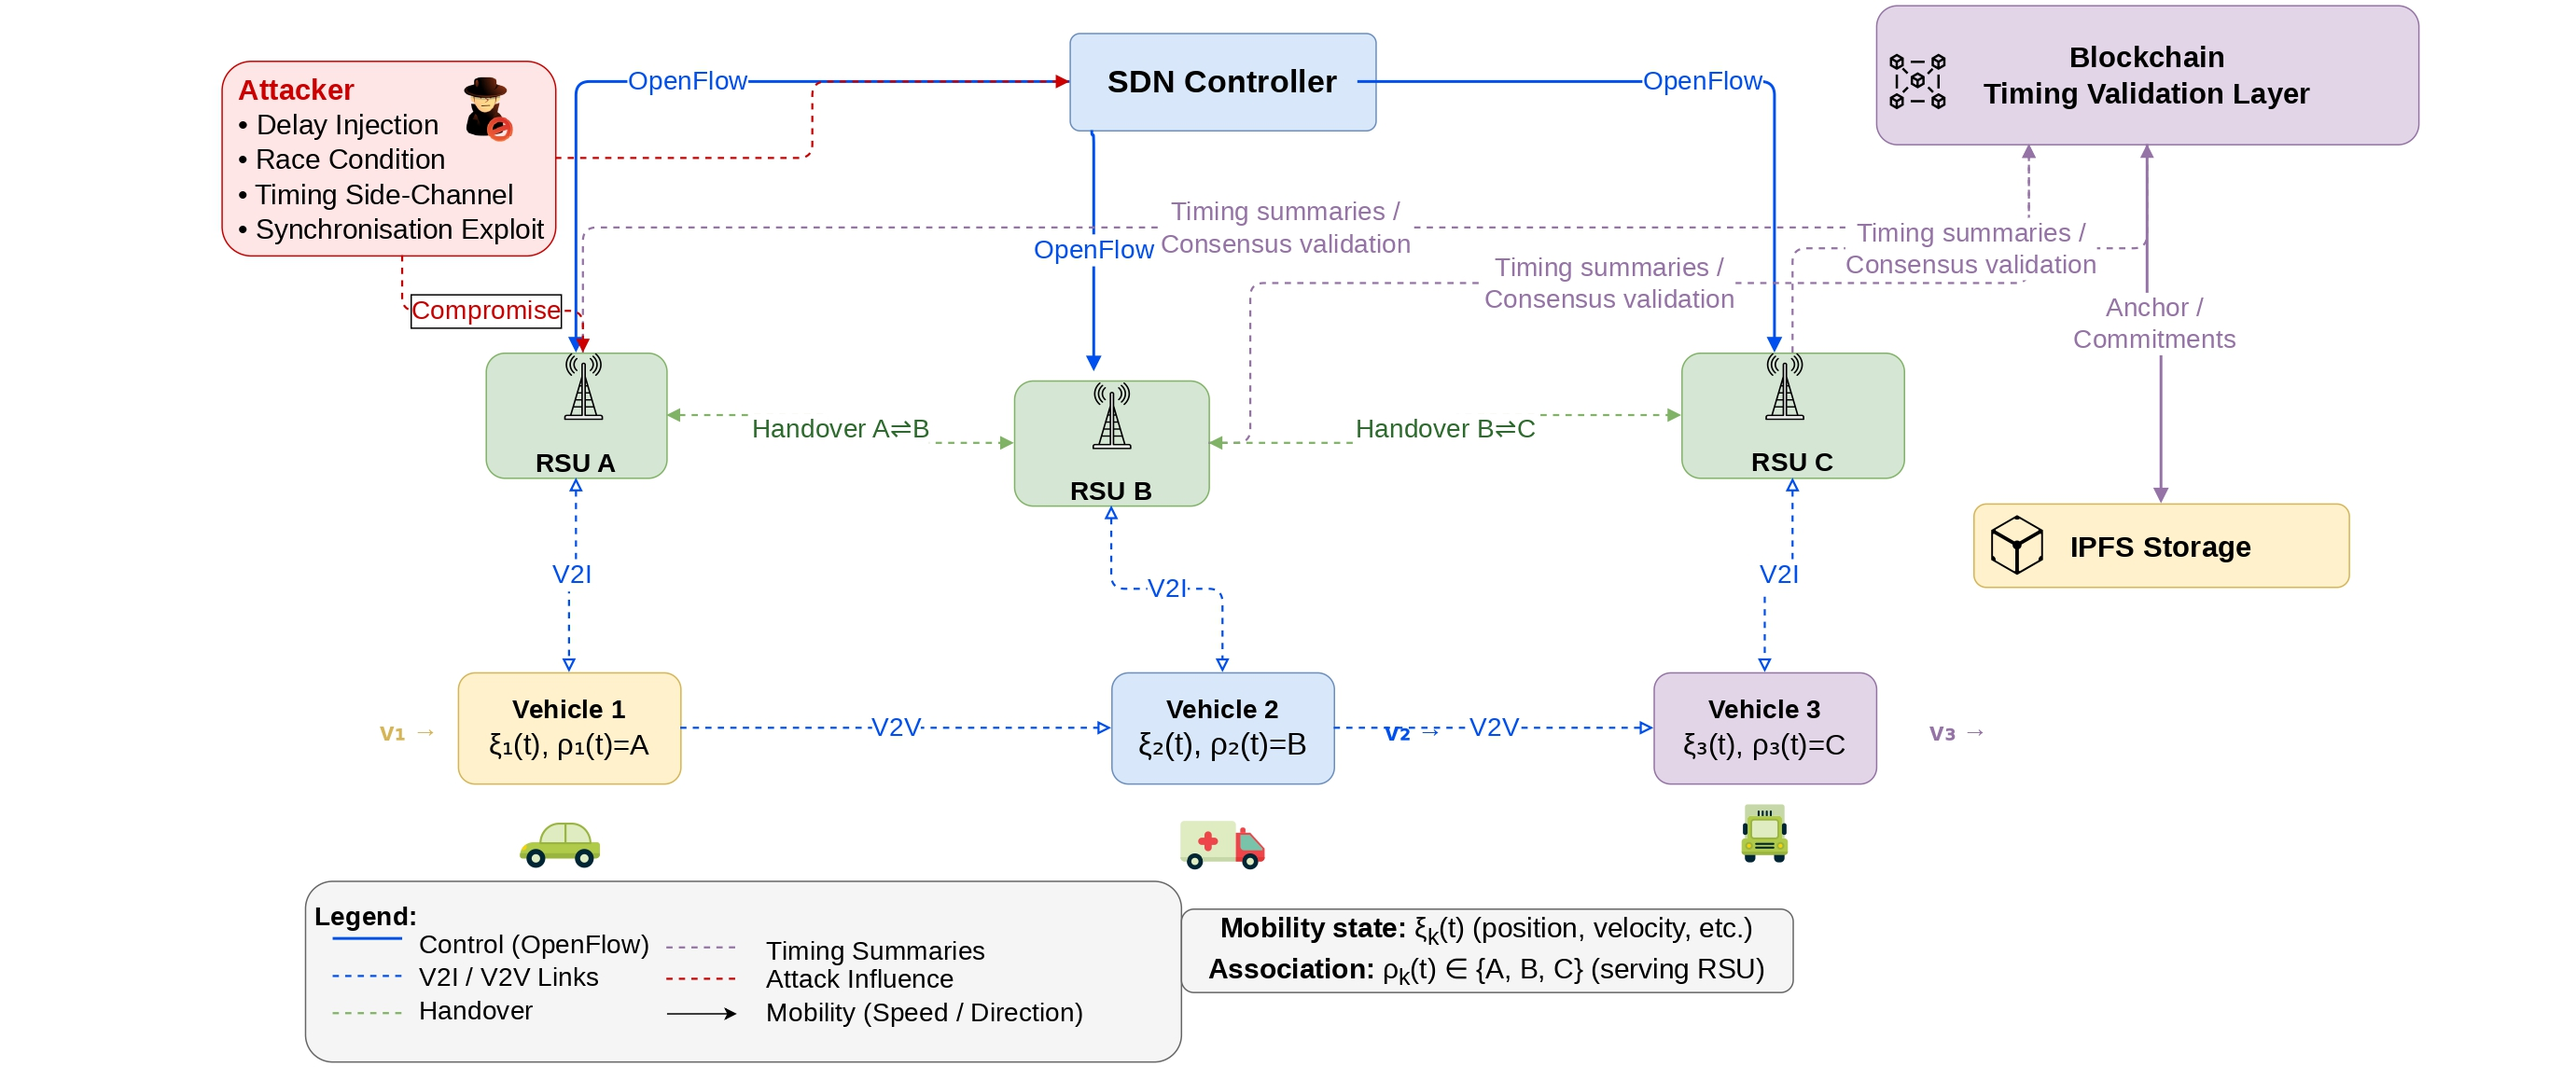
\includegraphics[width=0.9\linewidth]{system_model.jpg}
\caption{System model of the Software-Defined Vehicular Network with control-plane timing attack surface.}
\label{fig:system_model}
\end{figure}
\FloatBarrier
The system model that will be taken into account in the present study is depicted in Figure~\ref{fig:system_model}. The model is made up of a logically centralized SDN controller, several RSUs, mobile vehicular nodes, and distributed blockchain ledger. The SDN controller is in charge of world network monitoring, installation of flow-rules and timing sensitive control decisions. RSUs serve as bridges between the controller and the vehicles and transmit control-plane messages and send timing-related information. Cars communicate with RSUs through V2I and can be used to exchange safety-critical information through V2V.

The blockchain ledger is a decentralized timing validation layer, where RSUs and the controller store cryptographically verifiable timing summaries. Agreeing in RSUs enables the identification of timing anomalies without the use of a single trusted entity. An adversary can act as an external attacker that causes timing delays or act as an insider by a partial compromise of the RSU. These timing manipulations are aimed at control-plane messages travelling over OpenFlow channels so as to create the basis of the threat model and attack scenarios reported in the following sections.

IPFS provides content-addressable decentralised 
storage for timing proof commitments, enabling 
real-time evidence anchoring without blocking 
blockchain consensus. The mobility state of each 
vehicle $v_k$ is characterised by position, velocity, 
and current RSU association, which changes at 
handover events and directly amplifies the 
exploitability of timing attacks.

\subsection{Threat Model}

This study considers an adversary targeting the control plane of SDVN through timing manipulation. The threat model defines the attacker’s capabilities, limitations, and system assumptions under which the proposed defense framework operates.

\subsubsection{Attacker Capabilities}

The attacker is assumed to possess the following capabilities:
\begin{itemize}
    \item The ability to introduce bounded delays, reorder messages, or selectively drop control-plane packets between the controller, RSUs, and vehicles.
    \item The capability to compromise a limited number of RSUs or vehicular nodes, enabling insider timing manipulation.
    \item The ability to passively observe control-plane response times to infer timing-related information.
    \item The ability to exploit vehicular mobility and asynchronous network events to amplify timing inconsistencies.
\end{itemize}

\subsubsection{Attacker Limitations and Assumptions}

The following assumptions constrain the attacker:
\begin{itemize}
    \item Cryptographic primitives such as secure hash functions and digital signatures cannot be broken.
    \item The attacker cannot simultaneously compromise all controllers and RSUs.
    \item Encrypted and authenticated communication channels cannot be bypassed.
    \item Introduced delays remain within plausible network bounds to avoid immediate detection.
\end{itemize}

\begin{comment}
...
\end{comment}

\subsection{Attack Scenarios}

This section outlines the scenarios of control-plane timing attacks that are taken into account in this paper. All the attacks exploit timing vulnerabilities in SDVNs but do not alter the contents of packets. The scenarios are in agreement with the formulated threat model and form the foundation of the proposed defense formulation.

\subsubsection{Delay Injection Attack}

%
% ------------------------------------------------------------------
% Delay Injection Attack Scenarios
% ------------------------------------------------------------------
% Figure~\ref{fig:delay_attack} presents the two primary delay injection
% attack paths considered in the SDVN control-plane architecture. The
% attack targets timing-sensitive communications between the SDN controller,
% RSUs, and connected vehicles.
%
% In the downlink scenario shown in Figure~\ref{fig:delay_downlink},
% malicious entities introduce artificial delays into control messages
% transmitted from the SDN controller toward RSUs and vehicles. Since
% SDVN environments rely on rapid dissemination of routing and management
% instructions, delayed packets may result in outdated forwarding rules,
% increased end-to-end latency, reduced synchronization efficiency, and
% degradation of traffic management performance.
%
% In the uplink scenario shown in Figure~\ref{fig:delay_uplink}, the
% attacker delays telemetry, trust updates, and network-state information
% sent from vehicles or RSUs back to the controller. Such disruptions
% reduce the controller’s visibility of real-time network conditions,
% potentially affecting adaptive routing, trust computation accuracy,
% attack detection responsiveness, and overall network reliability.
%
% These bidirectional delay injection attacks demonstrate how timing
% manipulation can compromise SDVN control-plane stability and negatively
% impact throughput, latency, synchronization integrity, and trust-aware
% decision-making mechanisms.
% ------------------------------------------------------------------
%
% ====== FIGURE delay_attack — CORRECTED ======

Figure~\ref{fig:delay_attack} illustrates the delay injection
attack across both directions of SDVN control-plane
communication. The top panel shows the time axis: a control
message transmitted at $t_s^{ij}$ has a nominal expected
arrival at $t_1^{ij}$ (the TTL boundary $\tau_{\mathrm{TTL}}$),
but the attacker buffers the packet so that the observed
arrival $T_{\mathrm{obs}}^{ij}$ exceeds this boundary,
producing a deviation $\Delta\tau = T_{\mathrm{obs}}^{ij} -
t_1^{ij} > \theta_{\mathrm{DI}}$ as defined
in~\eqref{eq:sig_di}. The mobility context panel (top-right)
shows that high handover rate $H_{\mathrm{rate}}(t)$ generates
repeated flow-rule update events, each of which is an
independent injection window, directly corresponding to the
amplification factor $\Phi_{\mathrm{DI}}(t)$
in~\eqref{eq:phi_di}.

The downlink scenario (subfigure a) depicts an external
attacker buffering a Flow-Mod message between the SDN
controller and the RSU/Switch, causing the RSU to apply stale
forwarding rules to Vehicles~1--3. The consequence 
vehicles misrouted, safety messages delayed, emergency vehicle
affected  is highlighted in the red consequence box. The
uplink scenario (subfigure b) shows a compromised RSU
(insider) delaying a control message from Vehicle~$k$, which
causes the SDN controller to operate on outdated state and
apply stale rules, resulting in misrouting and real-world
harm.

\begin{figure}[htb]
\centering
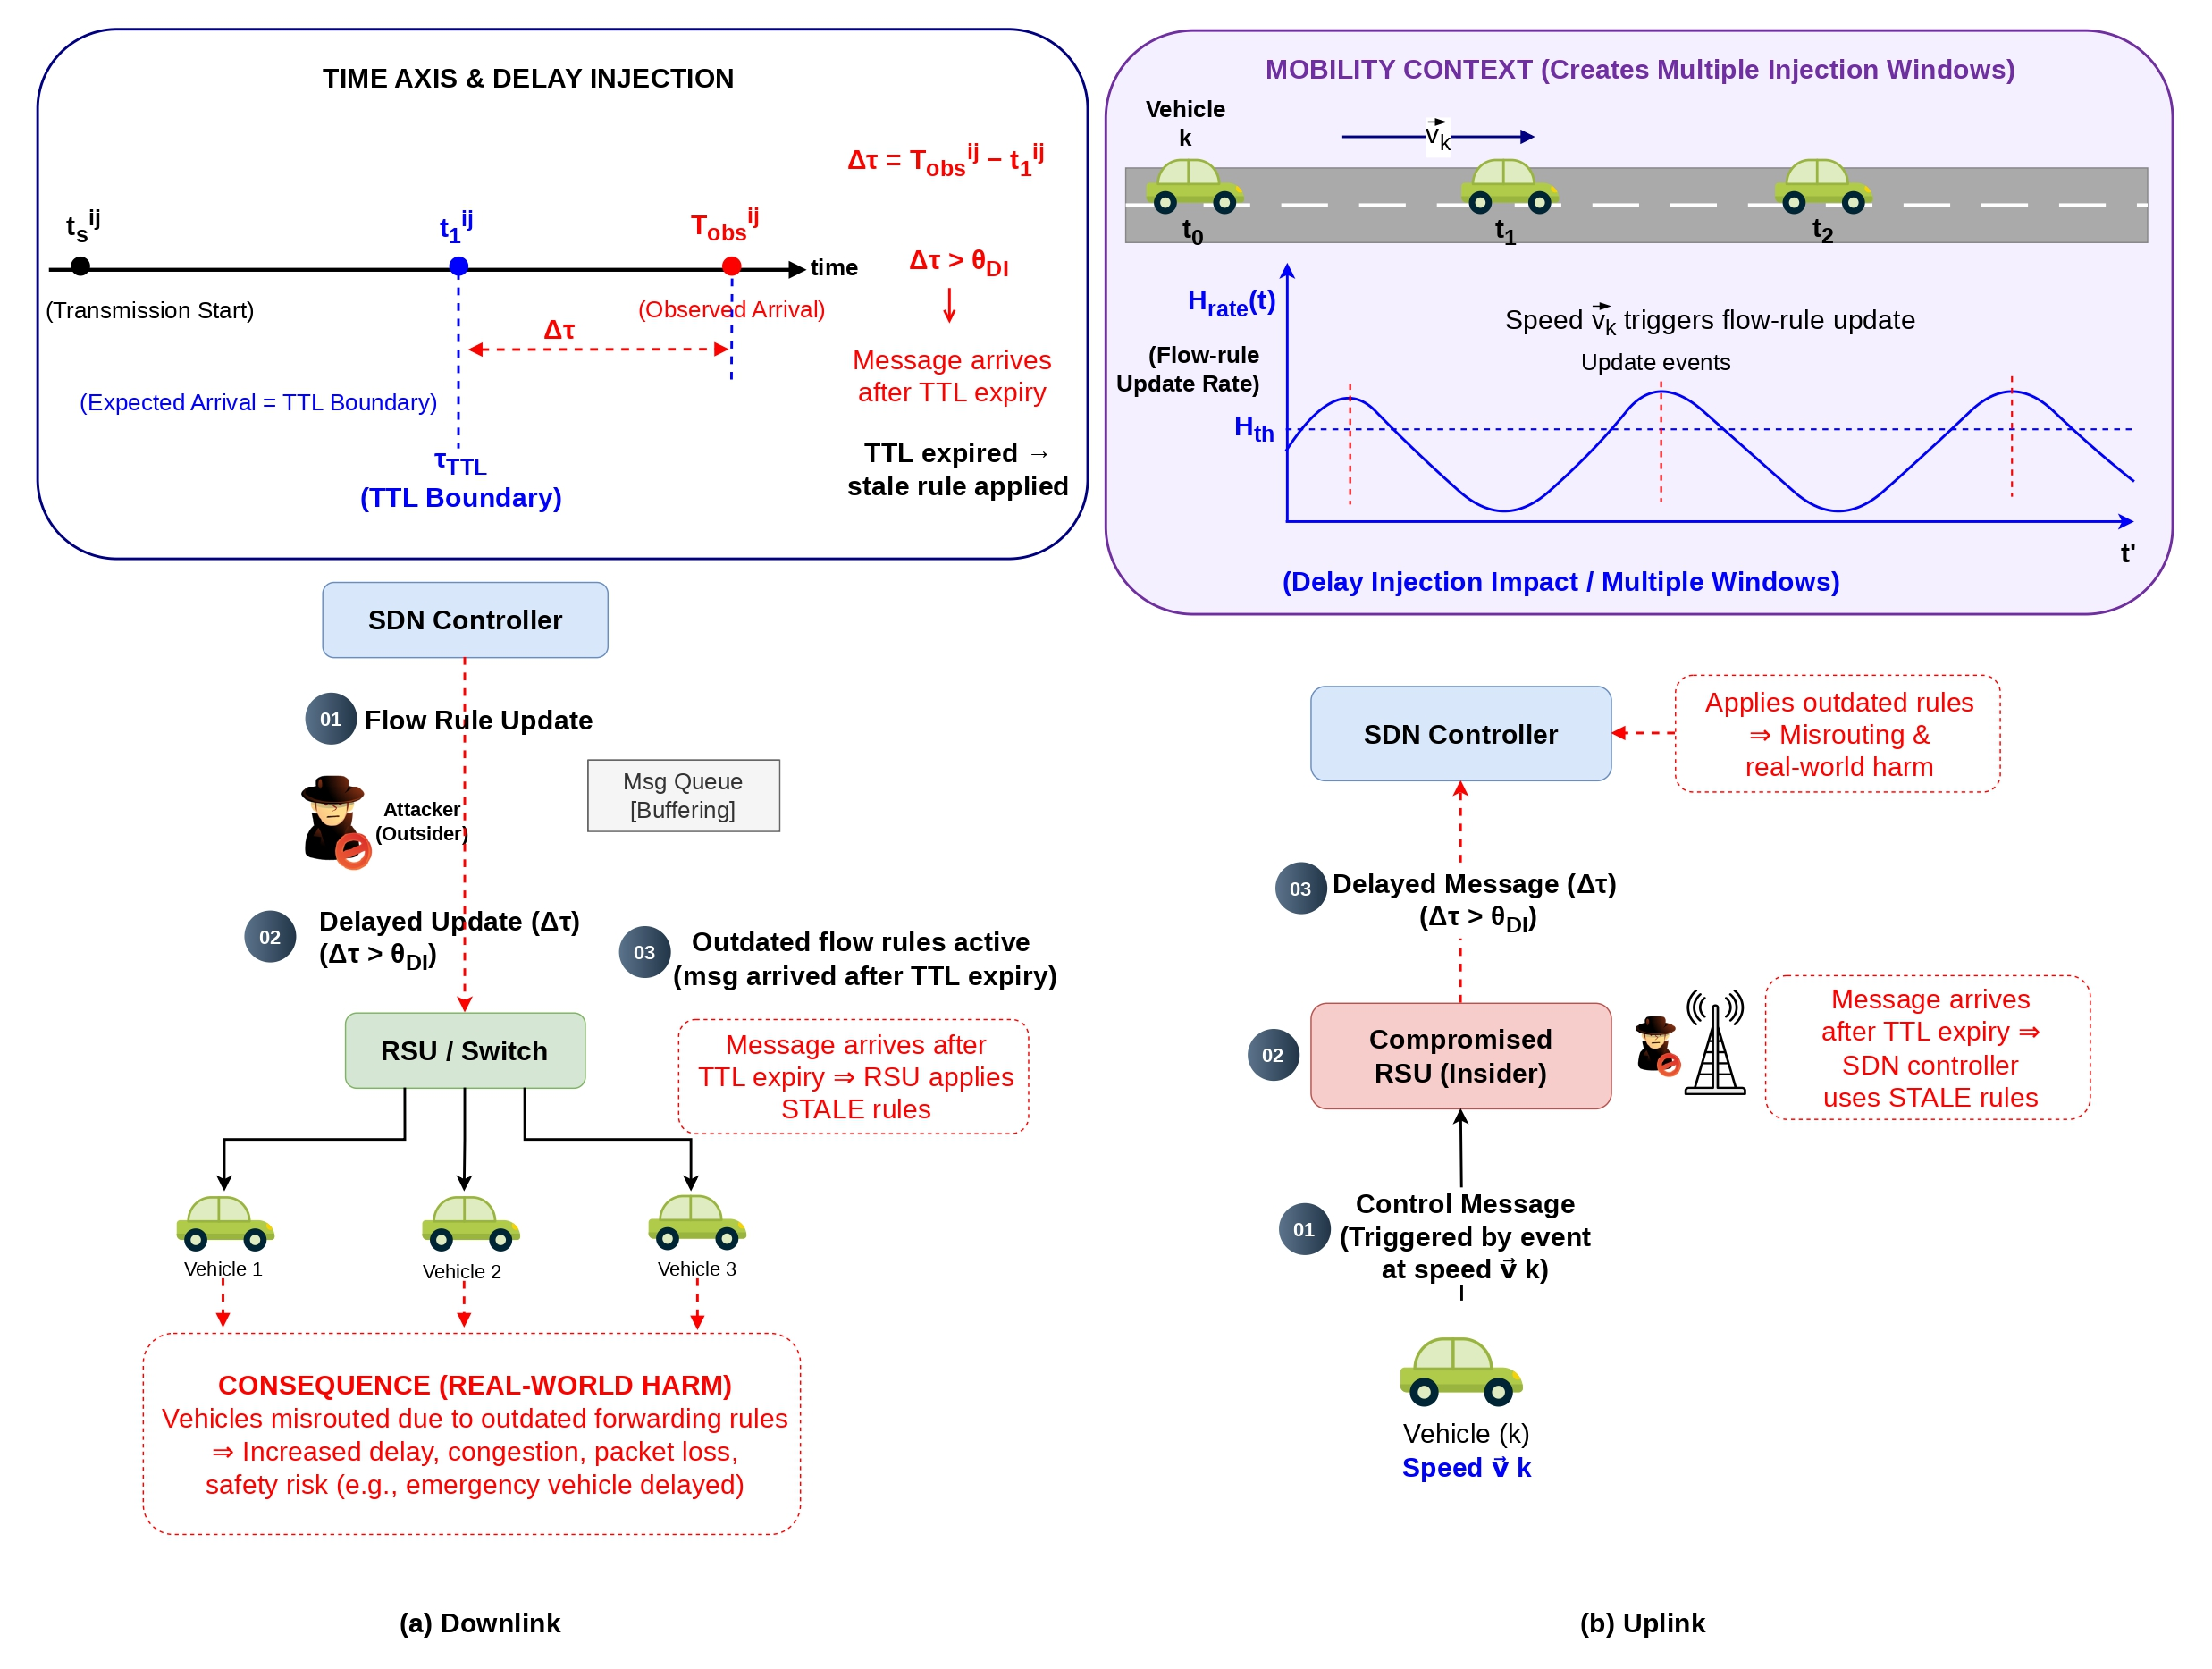
\includegraphics[width=\linewidth]{Progress_Works/all_timing_attacks/delay_injection_updated.jpg}
\caption{Delay injection attack in SDVN control-plane communication.}
\label{fig:delay_attack}
\end{figure}
\FloatBarrier
% ====== END FIGURE delay_attack ======

As shown in Figure~\ref{fig:delay_attack}, the attack
operates across both downlink and uplink directions, with the
attacker either buffering Flow-Mod messages from the controller
or delaying state reports from vehicles, in both cases causing
the controller or RSU to act on stale information with direct
consequences for vehicle routing and safety.

Delay injection attacks represent a critical threat to Software-Defined Vehicular Networks by intentionally manipulating the timing characteristics of control-plane communications without altering message content. These attacks exploit the time-sensitive nature of SDVN control operations to degrade network performance and compromise safety-critical vehicular applications. The attack manifests in two primary vectors: \textbf{downlink delay injection} (controller to RSU) and \textbf{uplink delay injection} (vehicle/RSU to controller).

\paragraph{Downlink Delay Injection Attack}
In the downlink scenario, the adversary targets flow rule updates transmitted from the SDN controller to Roadside Units (RSUs). The attack proceeds as follows:

\begin{enumerate}
    \item \textbf{Normal Flow Rule Update}: The SDN controller detects network events (vehicle movement, traffic priority changes, congestion, or safety message handling) and computes updated forwarding policies. This constitutes legitimate control-plane operation without malicious intent.
    
    \item \textbf{Malicious Delay Injection}: An external attacker intercepts the \textit{Flow-Mod} message and introduces an artificial delay $\Delta t$ by buffering or retarding the packet transmission. Crucially, the message content remains unaltered while its temporal delivery is manipulated.
    
    \item \textbf{Outdated Rule Application}: Due to the induced delay, the RSU fails to receive timely updates and continues operating with stale flow rules. This temporal discrepancy causes vehicles to be forwarded based on outdated network logic, potentially delaying safety messages, misrouting packets, or incorrectly handling traffic priorities.
\end{enumerate}

\paragraph{Uplink Delay Injection Attack}
In the uplink scenario, the attack targets control messages transmitted from vehicles or compromised RSUs to the SDN controller:

\begin{enumerate}
    \item \textbf{Vehicle/RSU Control Message}: A vehicle transmits control-plane messages (beacon timing, link quality measurements, handover status, or emergency indicators) to the RSU, expecting immediate forwarding to the controller.
    
    \item \textbf{Insider Delay by Compromised RSU}: A compromised RSU (insider attacker) intercepts the message and intentionally delays its transmission to the controller while preserving message integrity.
    
    \item \textbf{Delayed State Information}: The controller receives outdated network state information, leading to delayed or incorrect control decisions (e.g., late handover initiation after vehicle movement or delayed emergency response coordination).
\end{enumerate}

\begin{comment}
\paragraph{Integrated Mitigation Framework}
To counter delay injection attacks, we propose a multi-layered defense strategy that combines blockchain verification, adaptive learning, and intelligent analysis. The framework provides comprehensive protection through eight coordinated defense mechanisms:

\textbf{1. Access Control and Authentication:} For downlink protection, RSUs verify controller registration via blockchain smart contracts and accept only signed \textit{Flow-Mod} messages from authorized controllers. For uplink protection, the controller validates vehicle/RSU identities from the blockchain registry, rejecting unregistered or spoofed uplink messages. This ensures that only authenticated entities can participate in control-plane communications.

\textbf{2. Cryptographic Integrity:} In the downlink direction, the controller encrypts and digitally signs each \textit{Flow-Mod} message, with RSUs verifying signatures before rule application. For uplink communications, vehicles and RSUs sign uplink messages with their private keys, and the controller verifies these signatures to prevent message tampering. This cryptographic protection ensures message integrity even if transmission is delayed.

\textbf{3. Temporal Validation:} Downlink \textit{Flow-Mod} messages include essential timing metadata: \texttt{msg\_id}, \texttt{sequence\_no}, \texttt{timestamp}, and \texttt{TTL} (time-to-live). RSUs reject messages where the current time exceeds the timestamp plus TTL. Similarly, uplink messages contain \texttt{timestamp} and \texttt{nonce} values, with the controller discarding messages outside the acceptable freshness window and using nonces to prevent replay attacks. This ensures temporal consistency across all control-plane communications.

\textbf{4. Blockchain-based Timing Proof:} The controller stores hashes of \textit{Flow-Mod} metadata along with timestamps in IPFS, with the blockchain recording IPFS content identifiers (CIDs) and controller signatures. RSUs cross-verify timing against these blockchain records. For uplink protection, RSUs log uplink event timing hashes to IPFS, with the blockchain storing CIDs and RSU signatures. This provides immutable evidence for delay analysis and forensic investigation.

\textbf{5. Cross-Verification:} RSUs compare received flow rules with neighboring RSUs, triggering consensus validation when anomalies are detected. For uplink messages, the controller compares vehicle state information reported from multiple RSUs (RSU-A vs. RSU-B) and leverages V2V-assisted confirmation where available. Large discrepancies between reports indicate potential manipulation, enabling early detection of timing attacks.

\textbf{6. DRL-based Adaptive Response:} A deep reinforcement learning agent monitors \textit{Flow-Mod} delay patterns in the downlink direction, implementing actions such as reducing RSU trust scores, switching control paths, or enabling strict verification modes. The reward function encourages low-latency delivery while penalizing suspicious delays. For uplink protection, DRL analyzes delay deviations in conjunction with vehicle mobility patterns, link quality metrics, and trust scores. Adaptive responses include requesting re-validation, temporarily ignoring suspicious updates, using last-known-good states, or rerouting control to nearby RSUs.

\textbf{7. LLM Contextual Analysis:} Large Language Models analyze timing logs to classify delays as either "congestion-like" or "attack-like" patterns, generating human-readable alerts and mitigation recommendations. For uplink scenarios, LLMs correlate delay patterns with network conditions, providing contextual explanations such as "possible compromised RSU" or "network congestion scenario." This intelligent analysis supports forensic investigation and enhances decision-making for network operators.

\textbf{8. Trust Management:} Repeated late \textit{Flow-Mod} events reduce controller-RSU trust scores, potentially triggering quarantine modes for persistently delayed channels. Similarly, consistent uplink delays reduce vehicle/RSU trust scores, initiating probation periods with enhanced verification requirements. The system implements gradual trust restoration upon return to normal behavior, creating a dynamic trust ecosystem that adapts to evolving network conditions.

\paragraph{Mathematical Formulation of Delay Detection}
The temporal deviation metric for detecting delay injection attacks is extended to incorporate both downlink and uplink scenarios:

For downlink messages (controller $\rightarrow$ RSU):
\[
\Delta T_{\text{down}} = \left|T_{\text{obs}}^{\text{Flow-Mod}} - T_{\text{exp}}^{\text{Flow-Mod}}\right|
\]

For uplink messages (vehicle/RSU $\rightarrow$ controller):
\[
\Delta T_{\text{up}} = \left|T_{\text{obs}}^{\text{Packet-In}} - T_{\text{exp}}^{\text{Packet-In}}\right|
\]

Where $T_{\text{obs}}$ represents the observed arrival time and $T_{\text{exp}}$ denotes the expected arrival time derived from validated network state and propagation models. The system flags potential attacks when $\Delta T$ exceeds adaptive thresholds determined by DRL policy optimization, considering factors such as network congestion, vehicle velocity, and historical timing patterns.

\paragraph{Implementation Considerations}
The mitigation framework integrates with the proposed architecture through several key components:
\begin{itemize}
    \item \textbf{Smart Contracts}: Deployed on Hyperledger Fabric for decentralized registration, access control verification, and trust management
    \item \textbf{IPFS Integration}: Provides decentralized, tamper-proof storage for timing evidence and cryptographic proofs
    \item \textbf{DRL Agent}: Implemented using PyTorch and continuously trained on simulated attack scenarios to optimize response policies
    \item \textbf{LLM Module}: Fine-tuned on SDVN timing logs and attack patterns using Hugging Face Transformers for contextual threat intelligence
    \item \textbf{Consensus Mechanism}: Leverages Hyperledger Fabric's consensus protocol for cross-RSU timing validation and anomaly detection
\end{itemize}

This comprehensive approach ensures robust defense against delay injection attacks while maintaining the stringent low-latency requirements critical for safety-sensitive vehicular applications. The integrated framework provides proactive detection, adaptive response, and intelligent analysis capabilities that significantly enhance SDVN security against sophisticated timing-based threats. 
\newpage
\end{comment}

\subsubsection{Race Condition Exploitation}

%\begin{figure}[htbp]
%\centering
%\includesvg[width=0.85\linewidth]{race_condition_exploitation}
%\caption{Race condition exploitation through asynchronous control-plane updates.}
%\label{fig:race_condition}
%\end{figure}
%\FloatBarrier


% ====== FIGURE race_condition — CORRECTED ======

Figure~\ref{fig:race_condition} presents the race condition
attack in three complementary views. The top time axis shows
that a Link Up event $e_1$ is sent at $t_1$ and a
contradictory Link Down event $e_2$ follows at
$t_1 + \epsilon$, where $\epsilon = \epsilon_{\mathrm{RC}}$
is the exploitable race window. Both events trigger the
controller to generate Flow Mod~A and Flow Mod~B
respectively; these arrive at the RSU nearly simultaneously
($|t_b - t_a| \approx 0$), satisfying the conflict indicator
$\mathcal{C}(e_1, e_2) = -1$ in Equation~\eqref{eq:sig_rc}.
The mobility context panel (left) illustrates that rapid
vehicle movement causes a spike in link-event arrival rate
$\lambda_{\mathrm{event}}(t)$, creating more race windows and
directly increasing $\Phi_{\mathrm{RC}}(t)$ as given
in~\eqref{eq:phi_rc}.

The central diagram shows the attacker operating as a
compromised insider RSU, injecting contradictory events within
$\epsilon_{\mathrm{RC}}$ of each other. The consequence
(right) is an inconsistent flow table where two contradictory
rules  FORWARD and DROP for the same link  coexist
simultaneously, causing unpredictable routing behaviour.

\begin{figure}[htb]
\centering
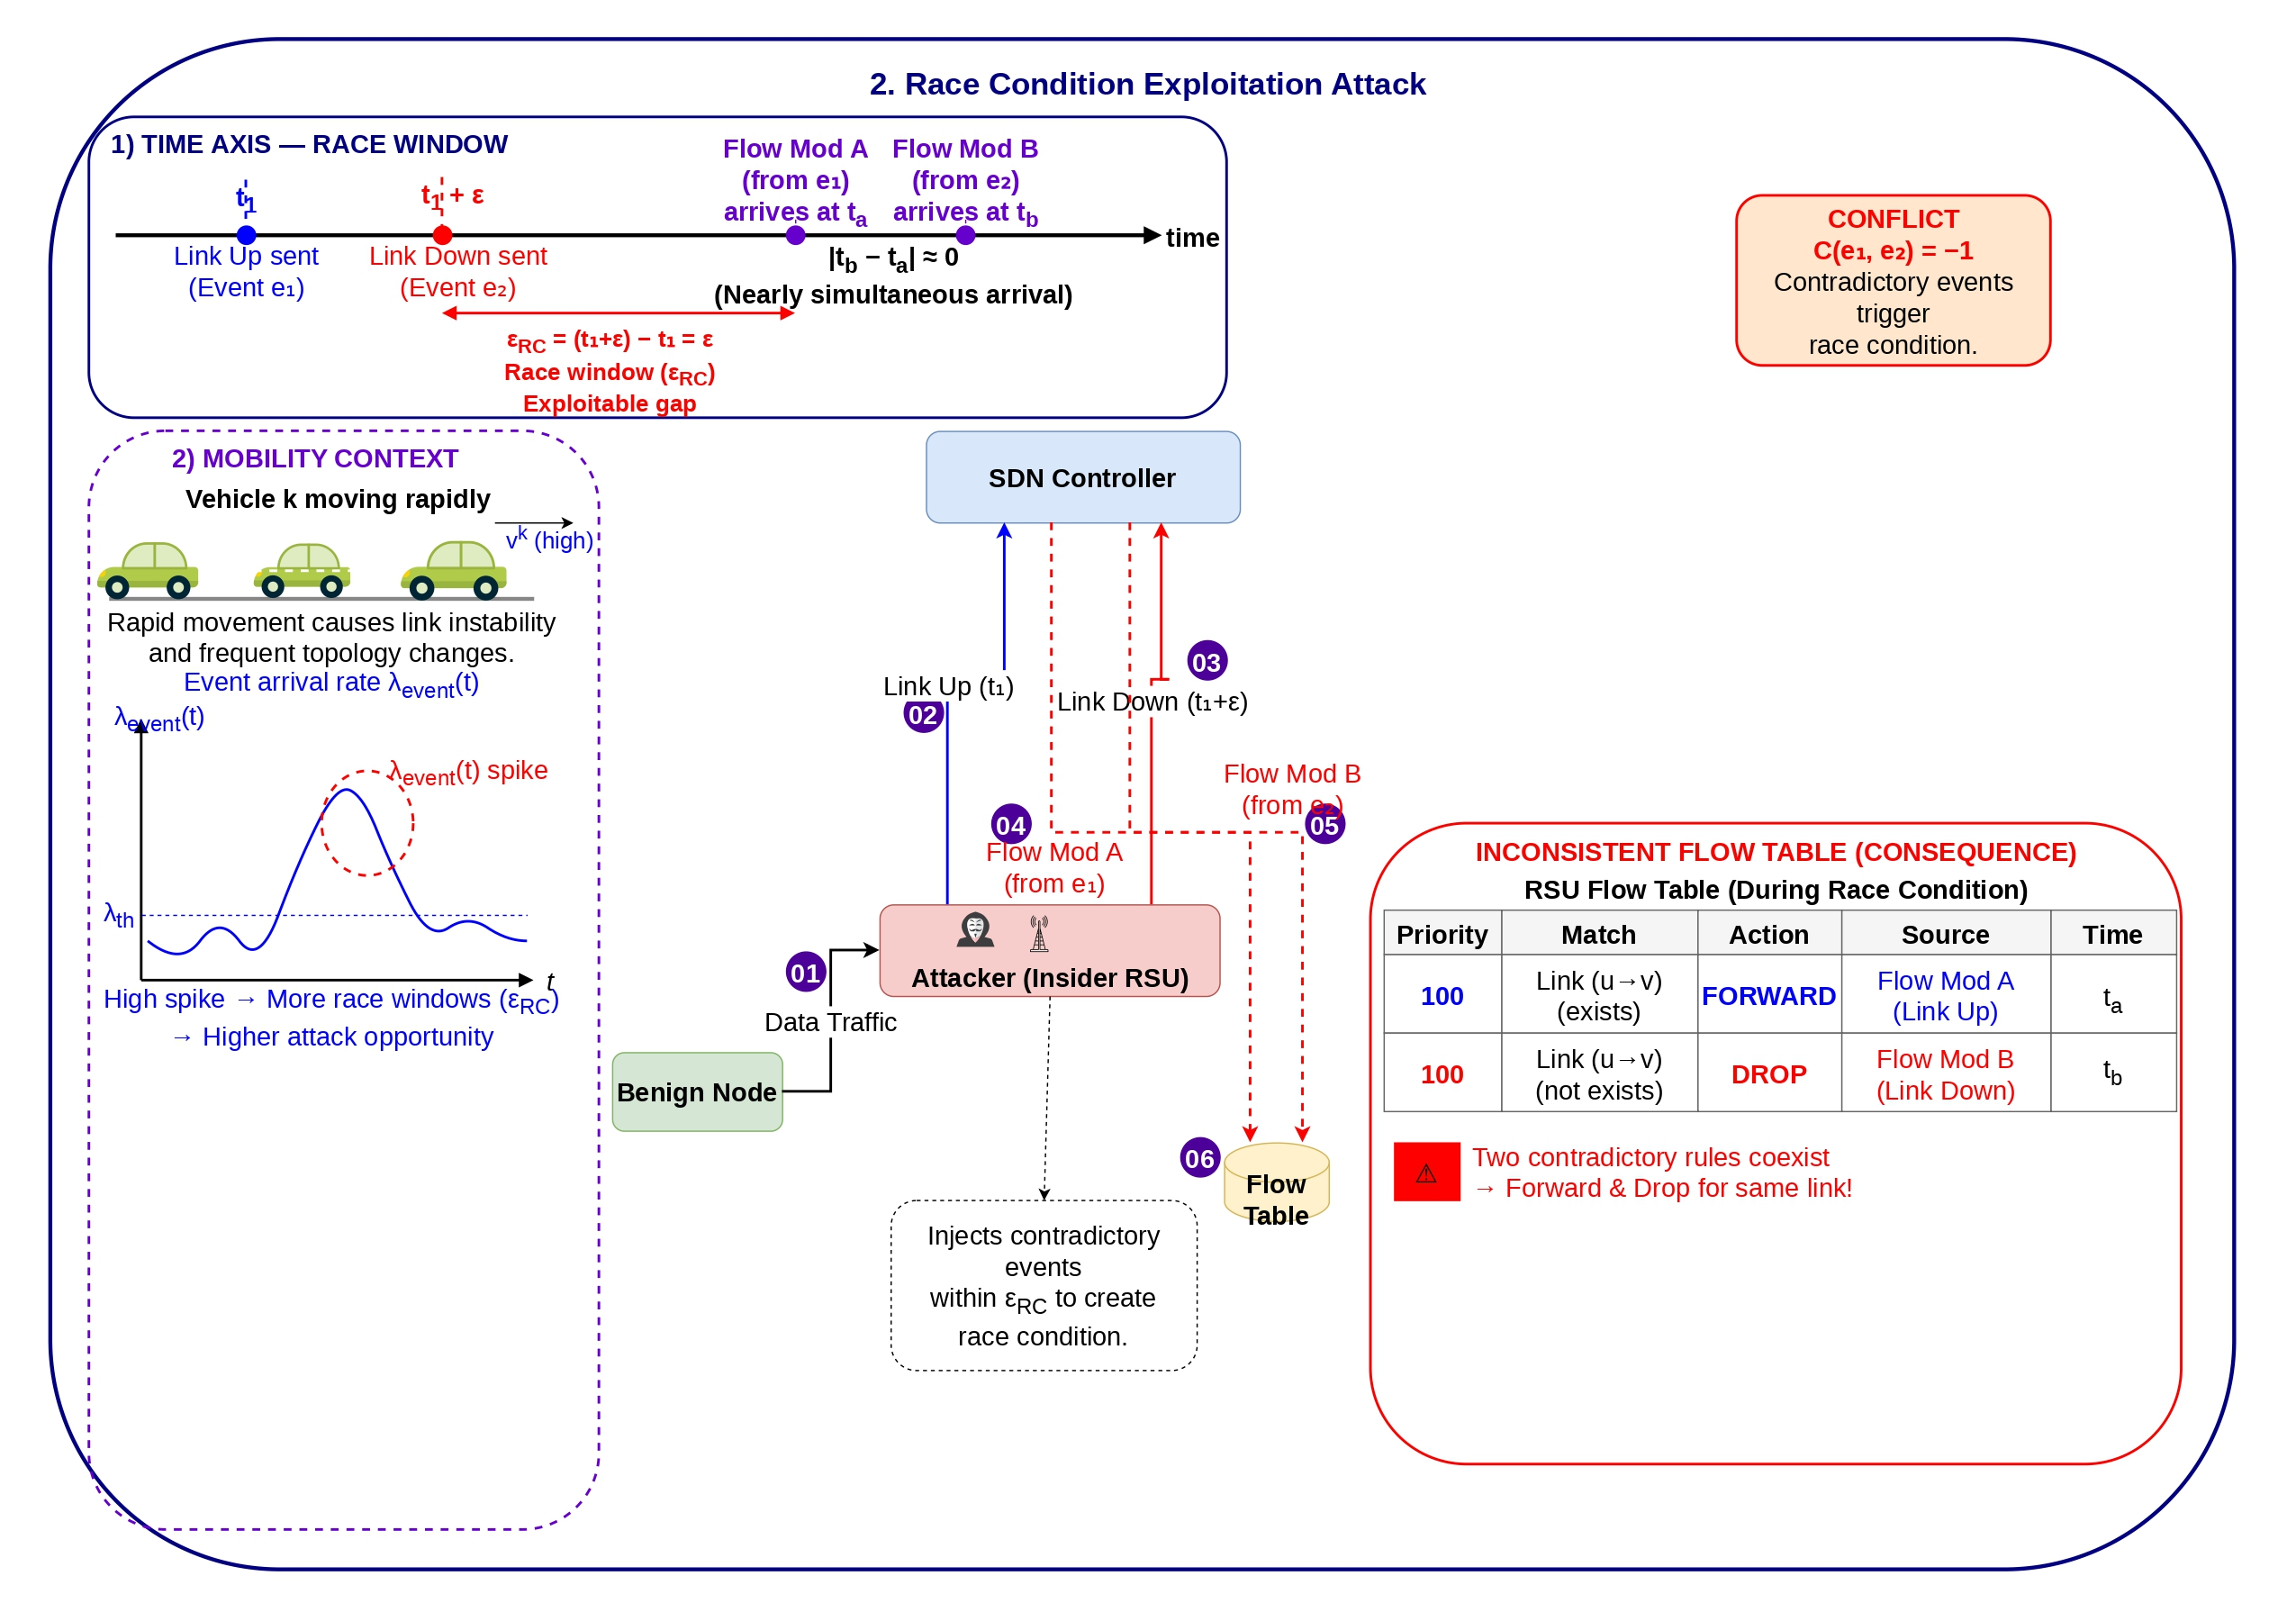
\includegraphics[width=\linewidth]{Progress_Works/all_timing_attacks/all_timing_attacks_page-0002.jpg}
\caption{Race condition exploitation through asynchronous control-plane updates.}
\label{fig:race_condition}
\end{figure}
\FloatBarrier
% ====== END FIGURE race_condition ======


As shown in Figure~\ref{fig:race_condition}, the attacker
injects contradictory Link Up and Link Down events within the
race window $\epsilon_{\mathrm{RC}}$, causing the controller
to generate conflicting Flow Mods that produce an inconsistent
flow table at the RSU with both FORWARD and DROP rules
coexisting simultaneously.

Race-condition exploitation represents a sophisticated timing attack where an adversary deliberately creates conflicting control-plane events that occur nearly simultaneously, causing the SDN controller to generate contradictory flow rules. Unlike protocol-based attacks, race conditions exploit timing dependencies in control-plane event processing, leveraging the asynchronous nature of SDVN updates to create network instability.

\paragraph{Attack Sequence and Mechanism}
The race condition attack unfolds through a carefully orchestrated sequence of events designed to create contradictory network state information:

\begin{enumerate}
    \item \textbf{Data Traffic (Benign Node $\rightarrow$ RSU)}: A legitimate vehicle or application initiates normal data traffic through the RSU, triggering monitoring events and activating link state evaluation mechanisms. This initial traffic is benign and serves as the catalyst for subsequent attack steps.
    
    \item \textbf{Link Up Event ($t_1 \rightarrow$ SDN Controller)}: The RSU detects acceptable link conditions based on recent measurements (beacon timing, packet arrival consistency, signal quality) and transmits a Link Up event to the SDN controller at time $t_1$. This event signals that the link is usable and prompts the controller to prepare appropriate forwarding rules.
    
    \item \textbf{Link Down Event ($t_1 + \epsilon \rightarrow$ SDN Controller)}: Shortly after the Link Up event (at time $t_1 + \epsilon$, where $\epsilon$ is extremely small), the same RSU sends a contradictory Link Down event indicating sudden link degradation. The attacker achieves this by manipulating timing measurements or report generation. This creates two contradictory link state reports that both appear temporally valid without requiring packet modification.
    
    \item \textbf{Flow Mod A Generation (Based on Link Up)}: The controller processes the Link Up event and generates Flow Mod A, which typically involves installing forwarding rules, allowing traffic flow, and prioritizing the specified link. This rule set is dispatched toward the RSU for implementation.
    
    \item \textbf{Flow Mod B Generation (Based on Link Down)}: Concurrently, the controller processes the Link Down event and generates contradictory Flow Mod B, which typically involves removing or downgrading rules, blocking traffic, or rerouting packets. This conflicting rule set is also dispatched toward the RSU.
    
    \item \textbf{Inconsistent Flow Table State}: Both Flow Mod A and Flow Mod B arrive at the RSU nearly simultaneously. Due to the asynchronous nature of control message processing and lack of strict ordering enforcement, the RSU processes them concurrently, resulting in an inconsistent flow table state where conflicting rules coexist. This inconsistency causes unpredictable network behavior, potential routing loops, or service disruption.
\end{enumerate}

\subsubsection{Timing Side-Channel Attack}

%\begin{figure}[htbp]
%\centering
%\begin{subfigure}{0.49\linewidth}
%  \centering
%  \includegraphics[width=\linewidth]{timingsidechannelattack1.png}
%  \caption{Passive Observation Phase}
%  \label{fig:timing_side_channel1}
%\end{subfigure}
%\hfill
%\begin{subfigure}{0.49\linewidth}
%  \centering
%  \includegraphics[width=\linewidth]{timingsidechannelattack2.png}
%  \caption{Timing Analysis Phase}
%  \label{fig:timing_side_channel2}
%\end{subfigure}
%\caption{Timing side-channel attack based on passive observation of control-plane responses.}
%\label{fig:timing_side_channel}
%\end{figure}
%\FloatBarrier

% ====== FIGURE timing_side_channel — CORRECTED ======

Figure~\ref{fig:timing_side_channel} illustrates the
three-phase timing side-channel attack. In the passive
observation phase (left panel), the attacker monitors
acknowledgement and packet timing between the SDN controller
and the RSU/Switch without injecting any traffic, collecting
a response-time sequence
$(T_1, T_2, \ldots, T_n)$. The statistical analysis phase
(centre panels) shows how the Pearson correlation
$\rho(\mathbf{T}_{1:n}, \mathbf{E}_{1:n})$ builds as more
samples are collected, approaching unity ($\rho \to 1$) over
$n_k$ samples  the condition captured by the signature
indicator $S_{\mathrm{SC}}$ in~\eqref{eq:sig_sc}. The
mobility amplification inset shows that higher vehicle density
$|\mathcal{V}_v(t)|$ and speed $\bar{v}(t)$ generate more
timing interactions, enlarging the attacker's statistical
corpus in accordance with
$\Phi_{\mathrm{SC}}(t)$~\eqref{eq:phi_sc}.

The active exploitation phase (right panel) depicts the
attacker acting as a fake controller under high-mobility
conditions, injecting a forged Flow-Mod with timing precisely
matching the inferred controller profile, causing the RSU to
install an incorrect flow rule and forward the vehicle to a
wrong destination.

\begin{figure}[htb]
\centering
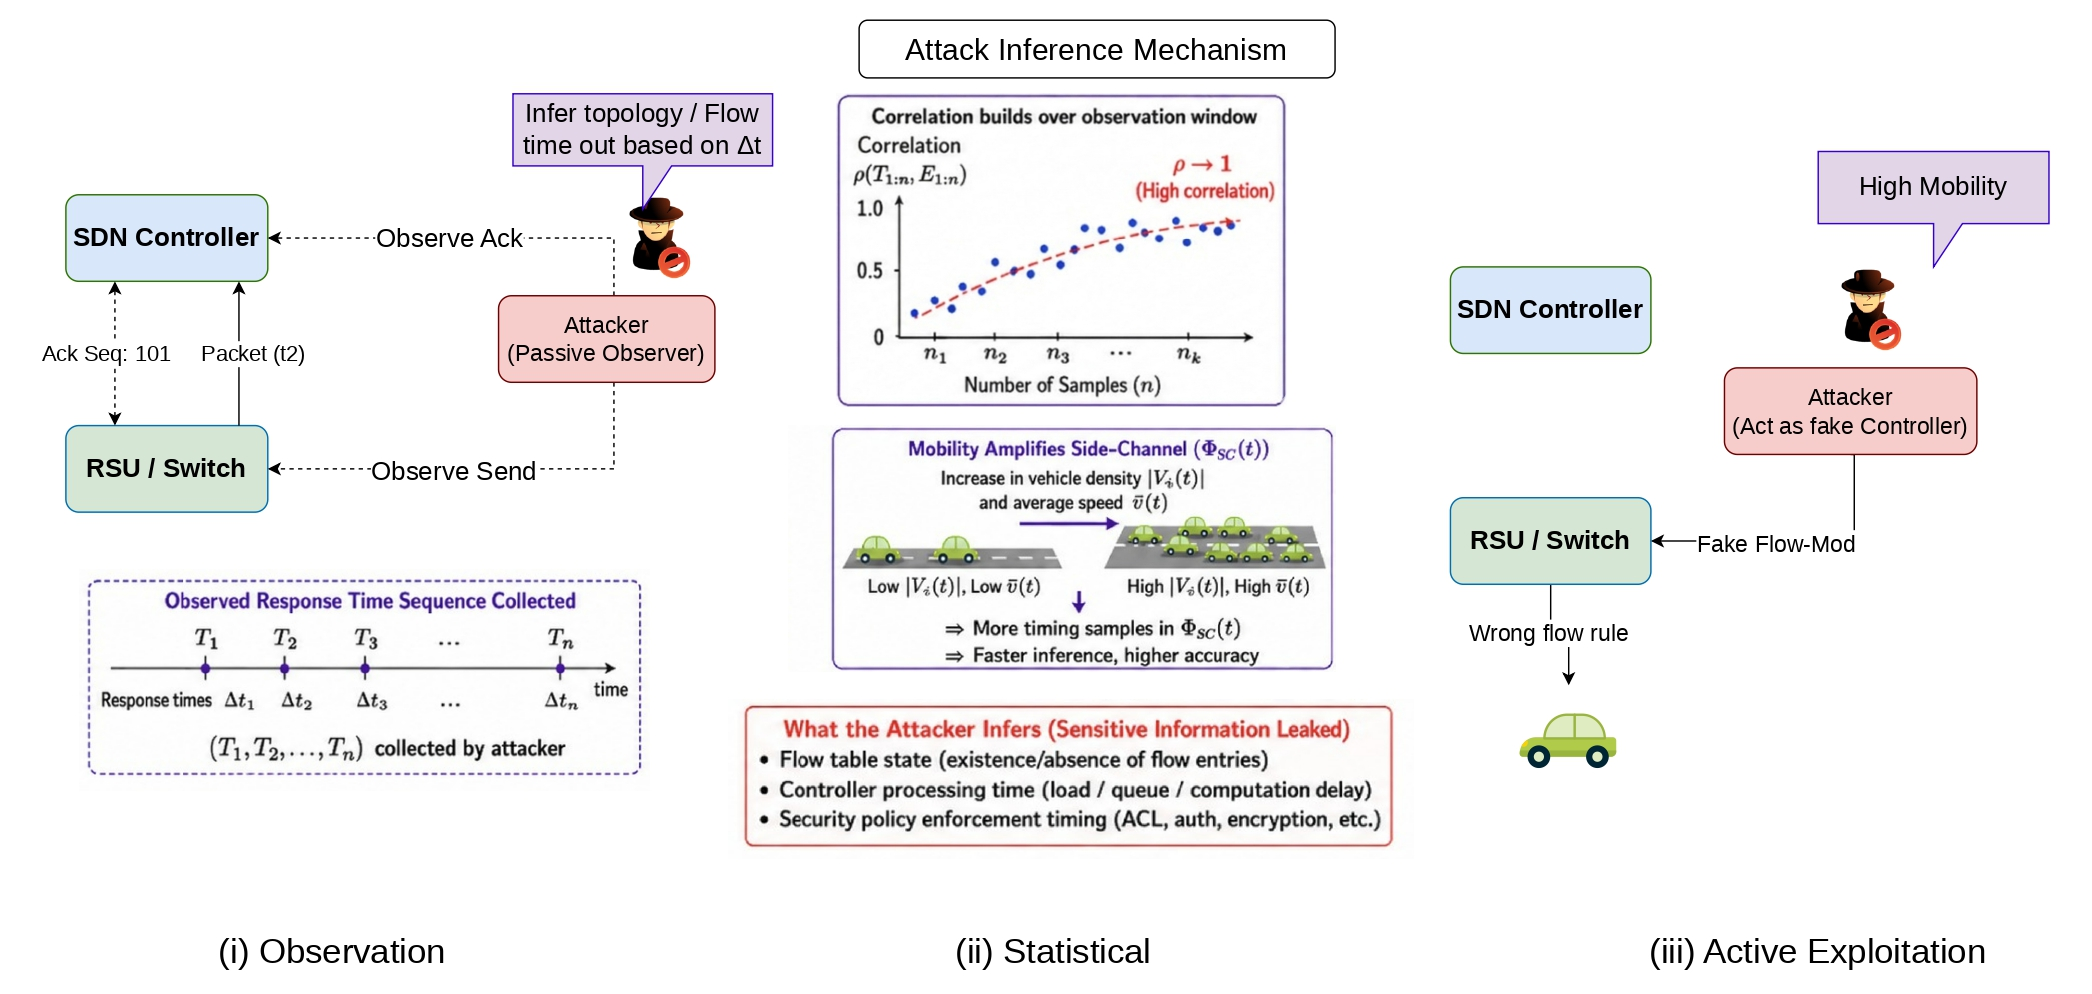
\includegraphics[width=\linewidth]{Progress_Works/all_timing_attacks/all_timing_attacks_page-0003.jpg}
\caption{Timing side-channel attack across three phases of passive observation, statistical analysis, and active exploitation.}
\label{fig:timing_side_channel}
\end{figure}
\FloatBarrier
% ====== END FIGURE timing_side_channel ======


As shown in Figure~\ref{fig:timing_side_channel}, the attack
progresses from passive collection of response-time sequences,
through Pearson correlation analysis that approaches unity as
the sample count grows, to active exploitation where the
attacker injects a forged Flow-Mod with timing matching the
inferred controller profile to install an incorrect flow rule.


Timing side-channel attacks represent a sophisticated security threat in Software-Defined Vehicular Networks where adversaries exploit temporal characteristics of control-plane communications to infer sensitive network information without direct packet manipulation. Unlike active attacks, timing side-channel attacks operate through passive observation and statistical analysis of timing patterns, enabling attackers to deduce critical network parameters, flow table states, and operational policies.

\paragraph{Attack Mechanism and Sequence}
Timing side-channel attacks leverage the correlation between control-plane response times and underlying network state. The attack proceeds through three sequential phases:

\begin{enumerate}
    \item \textbf{Passive Observation Phase}: During normal high-mobility vehicular operations, the attacker passively monitors control-plane communications between vehicles, RSUs, and the SDN controller. By logging traffic patterns, the attacker collects timing metadata including Flow-Mod response delays, acknowledgment intervals, round-trip times, and temporal variations in control message exchanges. This passive monitoring phase establishes baseline timing profiles without interfering with network operations.
    
    \item \textbf{Timing Analysis Phase}: Using statistical analysis and machine learning techniques, the attacker processes collected timing data to infer sensitive network information. Correlation analysis reveals relationships between timing patterns and specific network events, such as flow table updates, handover procedures, or congestion conditions. The attacker deduces critical parameters including controller processing times, network load characteristics, and security policy enforcement mechanisms.
    
    \item \textbf{Active Exploitation Phase}: Armed with detailed timing profiles, the attacker injects forged control-plane messages that mimic legitimate timing patterns. For example, the attacker crafts fake Flow-Mod packets with precisely calculated transmission delays that match expected controller response times. These carefully timed injections cause RSUs to accept incorrect flow rules, leading to misrouting, priority violations, or unauthorized network access.
\end{enumerate}

\textbf{Attack Impact}: Although timing side-channel attacks do not directly modify packet contents or disrupt network functionality, they enable sophisticated follow-on attacks by revealing critical timing dependencies. The extracted information can facilitate more targeted and successful timing-manipulation attacks, including precision delay injection, race condition exploitation, or synchronization manipulation. In high-mobility scenarios, attackers can leverage timing patterns to predict vehicle movements, anticipate handover events, or identify security policy enforcement mechanisms.


\begin{comment}
\paragraph{Integrated Mitigation Framework}
To counter timing side-channel attacks, we propose a comprehensive defense strategy that combines identity management, cryptographic protection, temporal validation, and intelligent analysis:

\textbf{1. Strict Identity Registration and Access Control}: Implement blockchain-based registration smart contracts that maintain cryptographic identities for all network entities (controllers, RSUs, vehicles). Only registered entities with valid public keys can participate in control-plane communications. This foundational layer prevents unauthorized entities from observing or injecting timing patterns.

\textbf{2. Mandatory Digital Signatures for Control Messages}: Require digital signatures on every Flow-Mod message using the controller's private key. RSUs verify signatures against registered public keys stored on the blockchain. Invalid signatures trigger immediate packet rejection, effectively preventing attackers from impersonating legitimate controllers or injecting forged timing patterns.

\textbf{3. Encrypted Channels with Mutual Authentication}: Establish encrypted control-plane channels with mutual authentication between controllers and RSUs. Encryption prevents passive observers from extracting timing information, while mutual authentication ensures both communication endpoints verify each other's identities before exchanging sensitive timing data.

\textbf{4. Temporal Validation with Sequence Numbers and TTL}: Include comprehensive timing metadata in control messages: \texttt{timestamp}, \texttt{sequence\_number}, and \texttt{TTL} (time-to-live). RSUs validate message freshness by checking that timestamps fall within acceptable windows, sequence numbers follow expected progressions, and packets arrive before TTL expiration. This prevents replay attacks and detects timing anomalies.

\textbf{5. Blockchain-IPFS Integration for Timing Proofs}: Controllers store hashes of Flow-Mod metadata along with precise timestamps in IPFS (InterPlanetary File System). The blockchain records IPFS content identifiers (CIDs) and controller signatures, creating immutable timing proofs. RSUs cross-verify received messages against these blockchain records to detect timing inconsistencies or tampering attempts.

\textbf{6. Flow-Table Consistency Checking}: Before installing new flow rules, RSUs perform consistency checks against existing rules and historical patterns. Anomalous rule changes, conflicting configurations, or abnormal update frequencies trigger verification requests to the controller or neighboring RSUs. This prevents inconsistent rule installations resulting from timing-based attacks.

\textbf{7. DRL-Based Adaptive Response System}: A deep reinforcement learning agent monitors timing patterns and implements adaptive responses based on observed deviations:
\begin{itemize}
    \item \textbf{State Representation}: Includes acknowledgment timing deviations, flow mismatch rates, node trust scores, vehicle mobility patterns, and link quality metrics.
    
    \item \textbf{Action Space}: Encompasses dropping suspicious updates, switching to alternate controller paths, increasing verification strictness levels, or quarantining suspicious network entities.
    
    \item \textbf{Reward Function}: Balances security effectiveness (correct attack detection) with network performance (minimizing legitimate operation disruption) and overhead considerations.
\end{itemize}

\textbf{8. LLM Contextual Analysis and Alert Generation}: Large Language Models analyze timing logs and security events to generate human-readable explanations and recommendations. LLMs classify timing patterns as legitimate (e.g., "congestion-induced delay") or malicious (e.g., "side-channel probing"), providing contextual insights that enhance operator decision-making and forensic analysis.

\paragraph{Mathematical Formulation of Timing Pattern Analysis}
The timing side-channel detection system employs statistical analysis to identify anomalous patterns:

\[
D_{\text{timing}} = \sqrt{\frac{1}{n} \sum_{i=1}^{n} (T_i - \mu_T)^2} \cdot \frac{|C(T_i, E_i)|}{\sigma_T}
\]

Where:
\begin{itemize}
    \item $D_{\text{timing}}$: Timing deviation score indicating potential side-channel activity
    \item $T_i$: Observed timing measurements (response times, acknowledgment delays)
    \item $\mu_T$, $\sigma_T$: Mean and standard deviation of legitimate timing patterns
    \item $C(T_i, E_i)$: Correlation coefficient between timing patterns and network events
    \item $n$: Number of timing observations in analysis window
\end{itemize}

High deviation scores combined with strong correlations between timing patterns and sensitive events trigger mitigation actions through the DRL agent.

\paragraph{Implementation and Integration}
The proposed mitigation framework integrates seamlessly with the overall defense architecture:

\begin{itemize}
    \item \textbf{Hyperledger Fabric Smart Contracts}: Manage identity registration, access control policies, and trust scoring mechanisms.
    
    \item \textbf{IPFS Distributed Storage}: Provides tamper-evident storage for timing proofs and cryptographic evidence.
    
    \item \textbf{PyTorch DRL Implementation}: Trains adaptive response policies using simulated timing side-channel attack scenarios in NS3.
    
    \item \textbf{Hugging Face Transformers}: Fine-tunes LLM models on SDVN timing logs to recognize side-channel patterns and generate contextual alerts.
    
    \item \textbf{NS3 Simulation Environment}: Validates defense effectiveness under various mobility patterns, network loads, and attack intensities.
\end{itemize}

This comprehensive approach provides robust protection against timing side-channel attacks by combining preventive measures (encryption, authentication), detective mechanisms (statistical analysis, DRL monitoring), and responsive actions (adaptive mitigation, intelligent alerts). The integrated framework ensures SDVN security while maintaining the low-latency performance critical for safety-sensitive vehicular applications.

\end{comment}

\subsubsection{Synchronization Exploits}

%\begin{figure}[htbp]
%\centering
%\begin{subfigure}{0.48\linewidth}
%  \centering
%  \includesvg[width=\linewidth]{Synchronization_Exploits_Beacon_Synchronization}
%  \caption{Beacon Synchronization Exploit}
%  \label{fig:sync_beacon}
%\end{subfigure}
%\hfill
%\begin{subfigure}{0.48\linewidth}
%  \centering
%  \includesvg[width=\linewidth]{Synchronization_Exploits_Handover_Synchronization}
%  \caption{Handover Synchronization Exploit}
%  \label{fig:sync_handover}
%\end{subfigure}
%\caption{Synchronization exploits targeting beacon transmission and handover coordination in SDVN.}
%\label{fig:synchronization_exploit}
%\end{figure}
%\FloatBarrier

% ====== FIGURE synchronization_exploit — CORRECTED ======

Figure~\ref{fig:synchronization_exploit} presents the two
synchronisation attack variants. The left panel depicts the
beacon synchronisation exploit: the expected beacon schedule
at the RSU (top sequence) shows periodic arrivals at intervals
$1/f_{\mathrm{beacon}}$, but the attacker jams beacons 2
and~3, creating a gap and introducing timing variance
$\sigma^2 > \theta_{\mathrm{SE}}^2$ as detected
by~\eqref{eq:sig_se}. This causes the RSU to report link
degradation (UP$\to$DOWN$\to$UP oscillation) and triggers
unnecessary flow rule reinstallations by the SDN controller.

The right panel illustrates the handover synchronisation
exploit. Vehicle~$k$ moves between the coverage areas of
RSU~A (source) and RSU~B (target). Under normal conditions,
RSU~A reports degrading link quality $A(t)$ and RSU~B reports
improving quality $B(t)$, enabling an accurate handover
decision. The attacker introduces a differential delay
$\Delta\tau_{\mathrm{arrival}}^{kr}(t) = t_B - t_A$ between
the two RSU measurement reports, as captured in
$\Phi_{\mathrm{SE}}(t)$~\eqref{eq:phi_se}. The SDN
controller consequently receives temporally inconsistent views
from RSU~A and RSU~B simultaneously, leading to a wrong
handover decision shown in the red consequence box
(top-right).

\begin{figure}[htb]
\centering
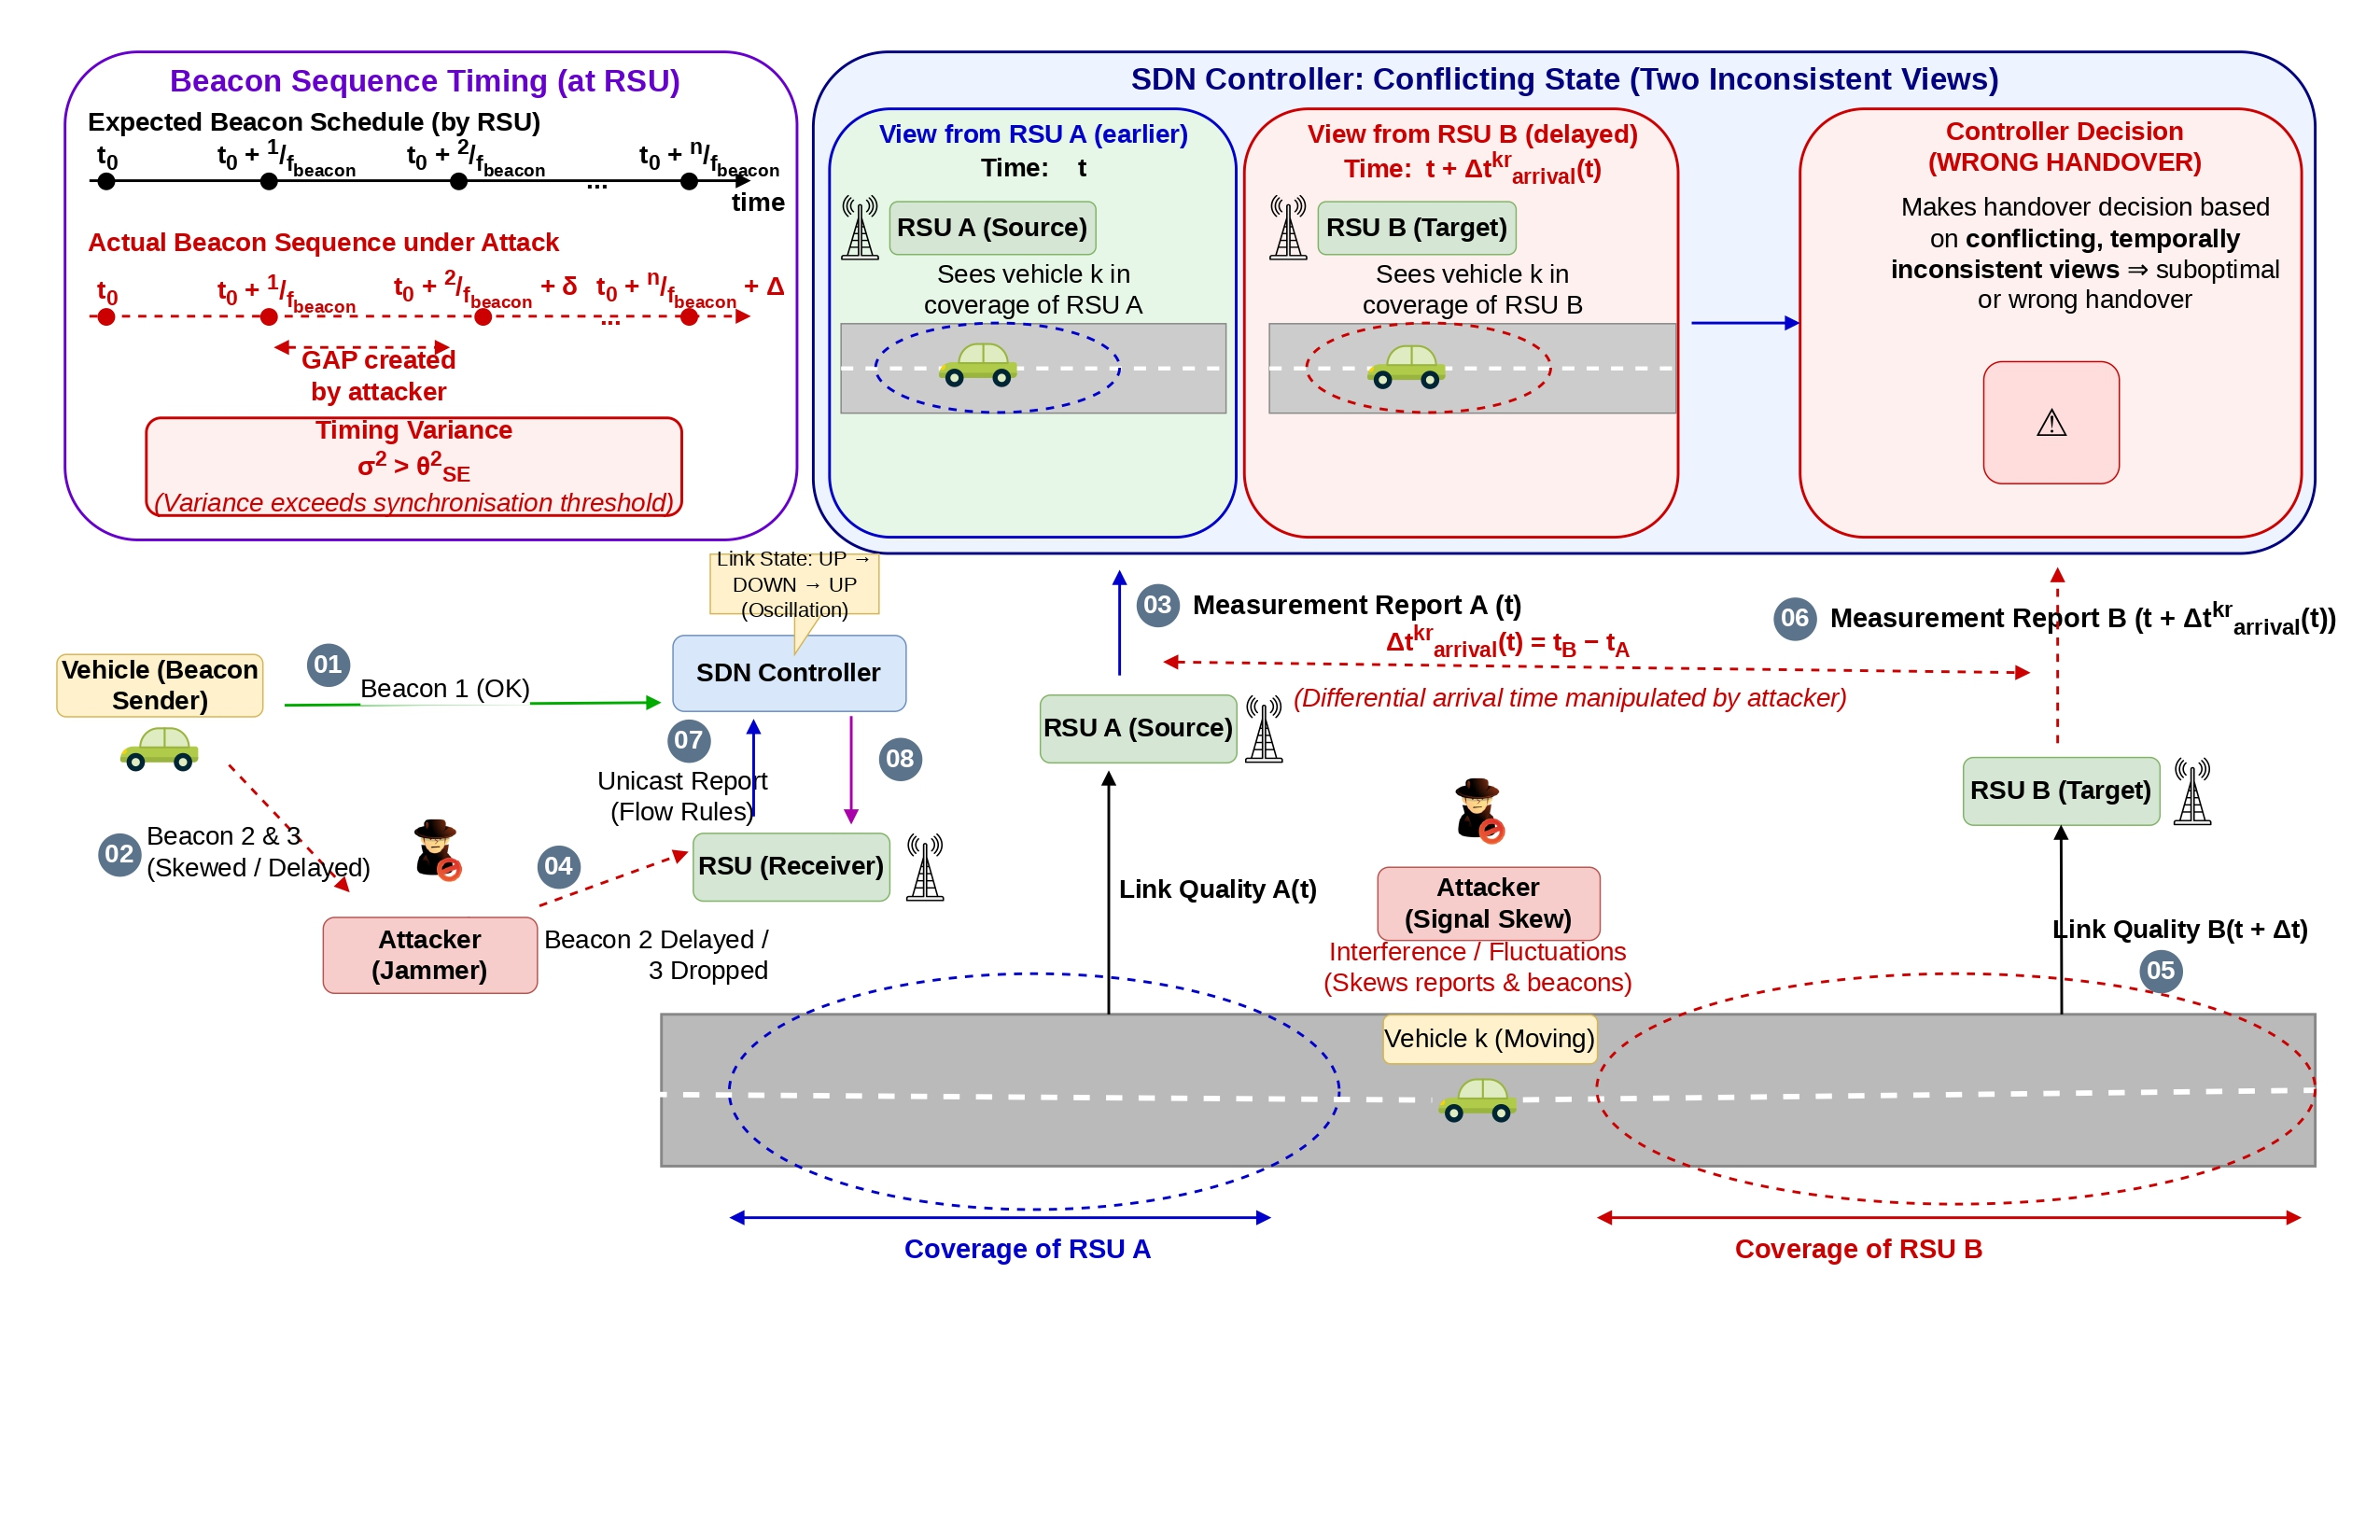
\includegraphics[width=\linewidth]{Progress_Works/all_timing_attacks/all_timing_attacks_page-0004.jpg}
\caption{Synchronisation exploits targeting beacon transmission and handover coordination in SDVN.}
\label{fig:synchronization_exploit}
\end{figure}
\FloatBarrier
% ====== END FIGURE synchronization_exploit ======

As shown in Figure~\ref{fig:synchronization_exploit}, the
beacon exploit creates inter-arrival gaps exceeding
$2/f_{\mathrm{beacon}}$ causing UP$\to$DOWN$\to$UP
oscillation at the RSU, while the handover exploit introduces
asymmetric differential delay $\Delta\tau_{\mathrm{arrival}}^{kr}$
between RSU~A and RSU~B reports, causing the controller to
make an incorrect handover decision.


Synchronization exploits represent sophisticated timing attacks that target coordination mechanisms in Software-Defined Vehicular Networks, particularly beacon transmission and handover synchronization. These attacks exploit the critical timing dependencies in vehicular coordination schemes by selectively delaying or dropping synchronization-related messages. The resulting inconsistent timing information propagation through RSUs and the SDN controller causes inaccurate handover judgments, connection retries, or intermittent communication failures. Such disruptions are particularly detrimental in high-mobility conditions where precise timing sensitivity is essential for effective vehicular coordination and safety-critical operations.

\paragraph{Handover Synchronization Exploit}
Handover synchronization exploits target the timing-sensitive process of transferring vehicle connectivity between Roadside Units during mobility. The attack mechanism involves strategic timing manipulation rather than content corruption:

\textbf{Attack Sequence:}
\begin{enumerate}
    \item \textbf{Vehicle Mobility Initiation}: A legitimate vehicle moves from the coverage area of RSU A toward RSU B, maintaining normal data connectivity throughout its trajectory.
    
    \item \textbf{Local Link Quality Measurement}: Both RSUs independently measure signal strength, RSSI (Received Signal Strength Indicator), SNR (Signal-to-Noise Ratio), and other link quality parameters. These measurements are locally accurate and reflect genuine network conditions.
    
    \item \textbf{RSU Report Transmission}: RSU A reports degrading link quality to the SDN controller, while RSU B reports improving link quality. Under normal conditions, these reports enable optimal handover decisions.
    
    \item \textbf{Selective Timing Manipulation}: The attacker implements asymmetric timing interference by delaying only one report path or introducing differential delays between report directions. Crucially, the attack does not corrupt report content or apply uniform delays to all communications.
    
    \item \textbf{Controller Decision Distortion}: The differential timing causes the SDN controller to receive reports in temporally distorted sequences, leading to incorrect handover decisions: premature handovers (if RSU A reports are delayed), late handovers (if RSU B reports are delayed), or handover oscillations (if reports arrive outside expected temporal windows).
\end{enumerate}

\textbf{Key Attack Characteristic}: The attack's effectiveness stems from \textit{relative timing manipulation} rather than absolute delay. Equal delays to both RSU reports would preserve correct relative timing and handover logic, while selective asymmetric delays create the conditions for incorrect decisions.

\paragraph{Beacon Synchronization Exploit}
Beacon synchronization exploits target periodic timing coordination messages that maintain network synchronization and location awareness:

\textbf{Attack Sequence:}
\begin{enumerate}
    \item \textbf{Normal Beacon Reception ($t_1$)}: The vehicle transmits periodic beacon $t_1$, which RSU receives normally, establishing correct synchronization baseline and confirming healthy link status.
    
    \item \textbf{Beacon Interception ($t_2$)}: The vehicle transmits beacon $t_2$, but an attacker jams or interferes with the wireless channel, preventing timely reception at the RSU.
    
    \item \textbf{Timing Manipulation ($t_2$ Delayed/$t_3$ Dropped)}: The attacker delays beacon $t_2$ and drops beacon $t_3$ entirely, creating observable gaps in beacon arrival patterns at the RSU.
    
    \item \textbf{Degraded Link State Reporting}: The RSU interprets missing beacons and timing inconsistencies as link degradation, transmitting unicast control reports to the SDN controller indicating unstable timing and perceived connectivity issues.
    
    \item \textbf{Network State Oscillation}: The controller updates network state views and flow rules based on distorted timing information, causing link state oscillations (UP $\rightarrow$ DOWN $\rightarrow$ UP) and repeated flow rule installations/removals that destabilize network operations.
\end{enumerate}


\begin{comment}
\paragraph{Integrated Mitigation Framework}
To counter synchronization exploits, we propose a multi-layered defense strategy combining identity management, cryptographic protection, temporal validation, and adaptive response mechanisms:

\textbf{For Handover Synchronization Protection:}
\begin{enumerate}
    \item \textbf{Blockchain-Based Registration}: Implement smart contracts that register all vehicles and RSUs, ensuring only authenticated entities participate in handover decisions.
    
    \item \textbf{Mutual Authentication with Digital Signatures}: Require digital signatures on all handover messages (vehicle requests, RSU acceptances, controller commands) to prevent unauthorized participation.
    
    \item \textbf{Encrypted Handover Control Channels}: Establish encrypted communication channels for handover coordination to prevent timing pattern analysis and injection attacks.
    
    \item \textbf{Spatio-Temporal Consistency Validation}: Include comprehensive metadata (timestamp, speed, direction vector, location) in handover requests, with verification against plausible mobility patterns and historical trajectories.
    
    \item \textbf{Blockchain-IPFS Evidence Storage}: Store tamper-proof handover event records (vehicle ID, source/destination RSUs, timing, location, decision) in IPFS with blockchain-anchored content identifiers for auditing and dispute resolution.
    
    \item \textbf{DRL-Based Handover Decision Optimization}: Implement DRL agents that consider multiple factors (RSSI trends, SINR, link duration predictions, vehicle speed, direction, timing deviations, RSU trust scores) to optimize handover timing and destination selection.
    
    \item \textbf{Oscillation Protection Mechanisms}: Detect and prevent ping-pong handovers through cooldown timers, hysteresis thresholds, and adaptive decision stabilization.
    
    \item \textbf{LLM Incident Interpretation}: Utilize Large Language Models to analyze handover patterns, distinguish between attack-induced instability and normal dense traffic variations, and generate actionable recommendations.
\end{enumerate}

\textbf{For Beacon Synchronization Protection:}
\begin{enumerate}
    \item \textbf{RSU Registration and Authentication}: Require blockchain-based registration of all RSUs, with vehicles accepting beacons only from authenticated sources.
    
    \item \textbf{Digitally Signed Beacons}: Implement digital signatures on all beacon messages, including timestamp, sequence number, RSU ID, and location hints for verification.
    
    \item \textbf{Selective Encryption}: Apply encryption to sensitive beacon fields (precise timing offsets, coordination metadata) to limit timing intelligence leakage.
    
    \item \textbf{Freshness Validation and Replay Protection}: Enforce strict freshness windows for beacon acceptance and implement nonce/sequence-based replay prevention.
    
    \item \textbf{Blockchain-IPFS Timing Anchoring}: Periodically store compact timing summaries (hashes of recent beacons with timestamps) in IPFS with blockchain anchoring for subsequent verification.
    
    \item \textbf{DRL-Based Anomaly Detection}: Deploy DRL agents at RSUs and vehicles to analyze beacon patterns (jitter, drift rates, packet loss, link quality, trust scores) and implement adaptive responses.
    
    \item \textbf{LLM Contextual Alerting}: Utilize LLMs to analyze beacon anomaly logs, generate human-readable explanations, and distinguish between attack patterns and benign network conditions.
\end{enumerate}

\paragraph{Mathematical Formulation of Synchronization Integrity}
The synchronization integrity metric evaluates timing consistency across multiple coordination mechanisms:

\[
S_{\text{sync}} = 1 - \frac{1}{n} \sum_{i=1}^{n} \frac{|T_i^{\text{obs}} - T_i^{\text{ref}}|}{\Delta T_{\text{max}}}
\]

Where:
\begin{itemize}
    \item $S_{\text{sync}}$: Synchronization integrity score (1 = perfect synchronization)
    \item $T_i^{\text{obs}}$: Observed timing of synchronization event $i$
    \item $T_i^{\text{ref}}$: Reference timing from validated sources
    \item $\Delta T_{\text{max}}$: Maximum allowable timing deviation
    \item $n$: Number of synchronization events in evaluation window
\end{itemize}

\paragraph{Implementation and Integration}
The proposed synchronization exploit mitigation integrates with the overall defense architecture:

\begin{itemize}
    \item \textbf{Hyperledger Fabric Smart Contracts}: Manage RSU and vehicle registration, authentication policies, and trust scoring for synchronization participants.
    
    \item \textbf{IPFS Distributed Storage}: Provide tamper-evident storage for synchronization event records and timing proofs.
    
    \item \textbf{PyTorch DRL Implementation}: Train adaptive handover and beacon synchronization policies using NS3-simulated attack scenarios.
    
    \item \textbf{Hugging Face Transformers}: Fine-tune LLM models on synchronization event logs to recognize attack patterns and generate contextual insights.
    
    \item \textbf{NS3 Simulation Environment}: Validate defense effectiveness under various mobility patterns, network densities, and attack strategies.
\end{itemize}

This comprehensive approach provides robust protection against synchronization exploits by combining preventive authentication, detective monitoring, and adaptive response mechanisms tailored to the specific characteristics of handover and beacon synchronization vulnerabilities in SDVN environments.

\end{comment}


\begin{comment}
    
\subsection{Attack Signature Identification and Lightweight Detection}
\label{sec:signatures}

Each timing attack variant is characterised by a measurable
\emph{attack signature} — a distinguishing temporal or statistical
observable that separates malicious from benign behaviour. These
signatures form the basis of the Lightweight (LW) detection mode and
also seed the DRL state vector in the Full mode.


    \begin{comment}
        
    \textbf{Delay Injection Signature (DI).}
    The attack produces a systematic positive temporal deviation exceeding
    a mobility-adapted threshold. Define the signature indicator as
    \begin{equation}
    S_{\mathrm{DI}}(m) =
      \begin{cases}
        1 & \text{if } T_{\mathrm{obs}}^{m} - T_{\mathrm{exp}}^{m}
            > \theta_{\mathrm{DI}}(\hat{v}_k,\hat{H}) \\
        0 & \text{otherwise,}
      \end{cases}
    \label{eq:sig_di}
    \end{equation}
    where $T_{\mathrm{obs}}^{m}$ is the observed arrival time,
    $T_{\mathrm{exp}}^{m}$ is derived from~\eqref{eq:expected}, and the
    adaptive threshold is
    \begin{equation}
    \theta_{\mathrm{DI}}(\hat{v}_k,\hat{H}) =
      \tau_{\mathrm{TTL}}\!\left(1 +
      \alpha_{\mathrm{DI}}\,\frac{\hat{v}_k}{v_{\max}}\right) - \epsilon_0,
    \label{eq:theta_di}
    \end{equation}
    adjusting for estimated vehicle speed $\hat{v}_k$ and channel
    quality $\hat{H}$, preventing false positives under high-mobility
    legitimate topology changes.

\textbf{Delay Injection Signature (DI).}
The attack produces a systematic positive temporal deviation
exceeding a mobility-adapted threshold. The delay injection
signature indicator is defined in Equation~\eqref{eq:sig_di}.
\begin{equation}
S_{\mathrm{DI}}(m) =
  \begin{cases}
    1 & \text{if } T_{\mathrm{obs}}^{m} - T_{\mathrm{exp}}^{m}
        > \theta_{\mathrm{DI}}(\hat{v}_k,\hat{H}) \\
    0 & \text{otherwise,}
  \end{cases}
\label{eq:sig_di}
\end{equation}
As shown in Equation~\eqref{eq:sig_di}, $T_{\mathrm{obs}}^{m}$
is the observed arrival time and $T_{\mathrm{exp}}^{m}$ is derived
from~\eqref{eq:expected}. The indicator fires when the temporal
deviation exceeds the mobility-adapted threshold
$\theta_{\mathrm{DI}}$, which is defined in
Equation~\eqref{eq:theta_di}.
\begin{equation}
\theta_{\mathrm{DI}}(\hat{v}_k,\hat{H}) =
  \tau_{\mathrm{TTL}}\!\left(1 +
  \alpha_{\mathrm{DI}}\,\frac{\hat{v}_k}{v_{\max}}\right) - \epsilon_0,
\label{eq:theta_di}
\end{equation}
As shown in Equation~\eqref{eq:theta_di}, the threshold scales
with estimated vehicle speed $\hat{v}_k$ and channel quality
$\hat{H}$, preventing false positives under high-mobility
legitimate topology changes.

\begin{comment}
\textbf{Race Condition Signature (RC).}
The attack is characterised by semantically contradictory link-state
events from the same RSU within a critical temporal window:
\begin{equation}
S_{\mathrm{RC}}(e_1, e_2) =
  \mathbb{1}\!\left[\mathcal{C}(e_1,e_2){=}{-}1\right]
  \cdot\mathbb{1}\!\left[|t_{e_1}{-}t_{e_2}| < \epsilon_{\mathrm{RC}}\right]
  \cdot\mathbb{1}\!\left[\mathrm{src}(e_1){=}\mathrm{src}(e_2)\right],
\label{eq:sig_rc}
\end{equation}
where $\mathcal{C}(e_1,e_2)\in\{-1,0,1\}$ is a conflict indicator
($-1$ for contradictory events such as simultaneous Link-Up and
Link-Down), $\epsilon_{\mathrm{RC}}$ is the race window, and the
third predicate requires the same source RSU to rule out legitimate
multi-RSU disagreement.


\textbf{Race Condition Signature (RC).}
The attack is characterised by semantically contradictory
link-state events from the same RSU within a critical temporal
window. The race condition signature indicator is defined in
Equation~\eqref{eq:sig_rc}.
\begin{equation}
S_{\mathrm{RC}}(e_1, e_2) =
  \mathbb{1}\!\left[\mathcal{C}(e_1,e_2){=}{-}1\right]
  \cdot\mathbb{1}\!\left[|t_{e_1}{-}t_{e_2}| < \epsilon_{\mathrm{RC}}\right]
  \cdot\mathbb{1}\!\left[\mathrm{src}(e_1){=}\mathrm{src}(e_2)\right],
\label{eq:sig_rc}
\end{equation}
As shown in Equation~\eqref{eq:sig_rc},
$\mathcal{C}(e_1,e_2)\in\{-1,0,1\}$ is a conflict indicator
($-1$ for contradictory events such as simultaneous Link-Up
and Link-Down), $\epsilon_{\mathrm{RC}}$ is the race window,
and the third predicate requires the same source RSU to rule
out legitimate multi-RSU disagreement. All three conditions
must hold simultaneously for the signature to fire.


\begin{comment}
\textbf{Timing Side-Channel Signature (SC).}
The attack manifests as an anomalously strong statistical correlation
between control-plane response times and discrete network events,
combined with unnaturally low timing jitter:
\begin{equation}
S_{\mathrm{SC}}(\mathbf{T}_{1:n}) =
  \mathbb{1}\!\left[\rho(\mathbf{T}_{1:n},\mathbf{E}_{1:n})
    > \rho_{th}\right]
  \cdot
  \mathbb{1}\!\left[\hat{\sigma}_{\mathrm{timing}}
    < \theta_{\mathrm{noise}}\right],
\label{eq:sig_sc}
\end{equation}
where $\rho(\cdot,\cdot)$ is the Pearson correlation between the
observed timing sequence $\mathbf{T}_{1:n}$ and network event
indicators $\mathbf{E}_{1:n}$, $\rho_{th}$ is the suspicious
correlation threshold, and $\hat{\sigma}_{\mathrm{timing}} 
\theta_{\mathrm{noise}}$ indicates the pattern is too regular to
arise from natural channel jitter.


\textbf{Timing Side-Channel Signature (SC).}
The attack manifests as an anomalously strong statistical
correlation between control-plane response times and discrete
network events, combined with unnaturally low timing jitter.
The timing side-channel signature indicator is defined in
Equation~\eqref{eq:sig_sc}.
\begin{equation}
S_{\mathrm{SC}}(\mathbf{T}_{1:n}) =
  \mathbb{1}\!\left[\rho(\mathbf{T}_{1:n},\mathbf{E}_{1:n})
    > \rho_{th}\right]
  \cdot
  \mathbb{1}\!\left[\hat{\sigma}_{\mathrm{timing}}
    < \theta_{\mathrm{noise}}\right],
\label{eq:sig_sc}
\end{equation}
As shown in Equation~\eqref{eq:sig_sc}, $\rho(\cdot,\cdot)$
is the Pearson correlation between the observed timing sequence
$\mathbf{T}_{1:n}$ and network event indicators
$\mathbf{E}_{1:n}$, and $\rho_{th}$ is the suspicious
correlation threshold. The second predicate checks that
$\hat{\sigma}_{\mathrm{timing}} < \theta_{\mathrm{noise}}$,
indicating the timing pattern is too regular to arise from
natural channel jitter. Both conditions must hold to reduce
false positives from congestion-induced correlation.

\begin{comment}
\textbf{Synchronisation Exploit Signature (SE).}
The attack produces detectable beacon gaps combined with
anomalously high inter-arrival variance:
\begin{equation}
S_{\mathrm{SE}}(\mathbf{b}_{1:n}) =
  \mathbb{1}\!\left[\exists\,k:\;b_k > \tfrac{2}{f_{\mathrm{beacon}}}
  \right]
  \cdot
  \mathbb{1}\!\left[\tfrac{1}{n}
    \sum_{i=1}^{n}(b_i-\bar{b})^2 > \theta_{\mathrm{SE}}^2\right],
\label{eq:sig_se}
\end{equation}
where $\mathbf{b}_{1:n}$ are beacon inter-arrival times; the first
predicate detects a missing beacon (gap exceeding two beacon periods)
and the second detects high temporal variance across the window.

\textbf{Synchronisation Exploit Signature (SE).}
The attack produces detectable beacon gaps combined with
anomalously high inter-arrival variance. The synchronisation
exploit signature indicator is defined in
Equation~\eqref{eq:sig_se}.
\begin{equation}
S_{\mathrm{SE}}(\mathbf{b}_{1:n}) =
  \mathbb{1}\!\left[\exists\,k:\;b_k > \tfrac{2}{f_{\mathrm{beacon}}}
  \right]
  \cdot
  \mathbb{1}\!\left[\tfrac{1}{n}
    \sum_{i=1}^{n}(b_i-\bar{b})^2 > \theta_{\mathrm{SE}}^2\right],
\label{eq:sig_se}
\end{equation}
As shown in Equation~\eqref{eq:sig_se}, $\mathbf{b}_{1:n}$
are beacon inter-arrival times. The first predicate detects a
missing beacon when the gap exceeds two beacon periods
$2/f_{\mathrm{beacon}}$, and the second detects high temporal
variance across the observation window. Both must be satisfied
simultaneously to distinguish an attack from transient channel
loss.


\begin{comment}
In LW mode, the HMAC-based lightweight authentication tag for each
control-plane message $m$ is computed as
\begin{equation}
\tau_{\mathrm{HMAC}}(m) =
  \mathrm{HMAC\text{-}SHA256}\!\left(K_s,\;
  m \,\|\, T_{\mathrm{obs}}^{m} \,\|\, \mathrm{seq}(m)\right),
\label{eq:hmac}
\end{equation}
where $K_s$ is the shared session key and $\mathrm{seq}(m)$ is a
monotonically increasing sequence number preventing replay. Any message
failing HMAC verification is immediately discarded before signature
evaluation.
In LW mode, the HMAC-based lightweight authentication tag for
each control-plane message $m$ is computed as given in
Equation~\eqref{eq:hmac}.
\begin{equation}
\tau_{\mathrm{HMAC}}(m) =
  \mathrm{HMAC\text{-}SHA256}\!\left(K_s,\;
  m \,\|\, T_{\mathrm{obs}}^{m} \,\|\, \mathrm{seq}(m)\right),
\label{eq:hmac}
\end{equation}
As shown in Equation~\eqref{eq:hmac}, $K_s$ is the shared
session key and $\mathrm{seq}(m)$ is a monotonically increasing
sequence number preventing replay attacks. Any message failing
HMAC verification is immediately discarded before signature
evaluation, ensuring unauthenticated messages never reach the
attack detection stage.

\begin{comment}
...
\end{comment}

% \subsection{Per-Variant Detection and Mitigation Algorithms}
% Algorithm~\ref{alg:di} covers the full detection and mitigation
% cycle for delay injection attacks, operating in both LW and Full
% modes. In LW mode, HMAC verification and threshold comparison
% provide immediate rejection; in Full mode, the DRL agent and
% smart contract provide adaptive enforcement.

% \begin{algorithm}[H]
% \caption{Delay Injection Detection and Mitigation
% (\texttt{DI-Defend})}
% \label{alg:di}
% \begin{algorithmic}[1]
% \small
% \Procedure{\texttt{DI-Defend}}
%   {$m,\hat{v}_k,\mathrm{mode},\pi_\theta,\mathrm{sk}_{\mathrm{ctrl}}$}
%   \State \textbf{--- Authentication ---}
%   \State Verify $\tau_{\mathrm{HMAC}}(m)$~\eqref{eq:hmac};
%     \textbf{if} invalid \textbf{then return} \textsc{Reject}
%   \State Verify $\mathrm{ML\text{-}DSA.Verify}
%     (\mathrm{pk}_{\mathrm{ctrl}},m,\sigma_m)$~\eqref{eq:verify};
%     \textbf{if} invalid \textbf{then return} \textsc{Reject}
%   \State Check nonce freshness and TTL;
%     \textbf{if} expired \textbf{then return} \textsc{Reject}
%   \State \textbf{--- Delay Detection ---}
%   \State $\Delta\tau \gets T_{\mathrm{obs}}^m - T_{\mathrm{exp}}^m$
%     \Comment{from~\eqref{eq:expected}}
%   \State $\theta_{DI} \gets \tau_{\mathrm{TTL}}
%     (1+\alpha_{DI}\hat{v}_k/v_{\max})-\epsilon_0$
%     \Comment{from~\eqref{eq:theta_di}}
%   \State $S_{DI} \gets \mathbb{1}[\Delta\tau > \theta_{DI}]$
%     \Comment{from~\eqref{eq:sig_di}}
%   \If{$S_{DI}=0$}
%     \State Accept $m$; update $\psi_r \uparrow$~\eqref{eq:trust_update}
%     \State \textbf{return} \textsc{Benign}
%   \EndIf
%   \State \textbf{--- Mode-Dependent Mitigation ---}
%   \If{$\mathrm{mode} = \mathrm{LW}$}
%     \State Discard $m$; log locally;
%       decrement $\psi_r \gets \psi_r - \Delta_{\mathrm{penalty}}$
%     \State \textbf{return} $(\textsc{Attack},\mathrm{DI},\Delta\tau)$
%   \EndIf
%   \State \textbf{--- Full Mode: DRL + Blockchain ---}
%   \State $\pi_{\mathrm{ZKP}} \gets \mathrm{ZKProve}
%     (T_{\mathrm{obs}}^m, \theta_{DI})$~\eqref{eq:zkp_prove}
%   \State $C_m \gets \mathrm{Hash}
%     (m\|\Delta\tau\|\pi_{\mathrm{ZKP}}\|\sigma_m)$
%     \Comment{from~\eqref{eq:commitment}}
%   \State $\mathrm{CID} \gets \mathrm{IPFS\_Store}(C_m)$
%     \Comment{from~\eqref{eq:cid}}
%   \State \texttt{SmartContract.SubmitTimingProof}
%     $(r,C_m,\sigma_r)$~\Comment{Alg.~\ref{alg:sc}}
%   \State $\mathbf{s}_t \gets \texttt{BuildState}
%     (\Delta\tau,\boldsymbol{\psi},\boldsymbol{\xi},
%     \mathbf{h}^{\mathrm{ctx}})$~\eqref{eq:state}
%   \State $a_t \gets \pi_\theta(\mathbf{s}_t)$
%     \Comment{from~\eqref{eq:actions}}
%   \If{$a_t \in \{a_2^{\mathrm{isolate}},a_3^{\mathrm{reroute}}\}$}
%     \State \texttt{PQC-Mitigate}$(r,\mathrm{DI},
%       \mathrm{sk}_{\mathrm{ctrl}})$~\Comment{Alg.~\ref{alg:pqc}}
%   \EndIf
%   \State \textbf{return} $(\textsc{Attack},\mathrm{DI},
%     a_t,\mathrm{CID})$
% \EndProcedure
% \end{algorithmic}
% \end{algorithm}


% Algorithm~\ref{alg:rc} handles race condition exploitation
% by detecting contradictory event pairs and enforcing atomic
% flow-rule update semantics via smart contracts in Full mode.

% \begin{algorithm}[H]
% \caption{Race Condition Detection and Mitigation
% (\texttt{RC-Defend})}
% \label{alg:rc}
% \begin{algorithmic}[1]
% \small
% \Procedure{\texttt{RC-Defend}}
%   {$e_{\mathrm{new}},\mathcal{Q},\mathrm{mode},
%   \pi_\theta,\mathrm{sk}_{\mathrm{ctrl}}$}
%   \State \textbf{--- Event Queue Inspection ---}
%   \State Append $e_{\mathrm{new}}$ to event queue $\mathcal{Q}$
%   \For{each $e_{\mathrm{prev}} \in \mathcal{Q}$
%     from $\mathrm{src}(e_{\mathrm{new}})$}
%     \State $\mathcal{C} \gets
%       \mathrm{ConflictCheck}(e_{\mathrm{prev}},e_{\mathrm{new}})$
%       \Comment{from~\eqref{eq:sig_rc}}
%     \State $\Delta t \gets |t_{e_{\mathrm{new}}}
%       - t_{e_{\mathrm{prev}}}|$
%     \If{$\mathcal{C}=-1$
%         \textbf{and} $\Delta t < \epsilon_{RC}$}
%       \State $S_{RC} \gets 1$; break
%     \EndIf
%   \EndFor
%   \If{$S_{RC}=0$}
%     \State Process $e_{\mathrm{new}}$ normally;
%       generate Flow-Mod
%     \State \textbf{return} \textsc{Benign}
%   \EndIf
%   \State \textbf{--- Mode-Dependent Mitigation ---}
%   \If{$\mathrm{mode} = \mathrm{LW}$}
%     \State Hold both conflicting Flow-Mods;
%       request re-report from RSU
%     \State Decrement
%       $\psi_r \gets \psi_r - \Delta_{\mathrm{penalty}}$
%     \State \textbf{return}
%       $(\textsc{Attack},\mathrm{RC},e_{\mathrm{prev}},
%       e_{\mathrm{new}})$
%   \EndIf
%   \State \textbf{--- Full Mode: Atomic Enforcement ---}
%   \State $\mathbf{s}_t \gets \texttt{BuildState}
%     (\Delta\tau^{RC},\boldsymbol{\psi},\boldsymbol{\xi},
%     \mathbf{h}^{\mathrm{ctx}})$~\eqref{eq:state}
%   \State $a_t \gets \pi_\theta(\mathbf{s}_t)$
%   \If{$a_t = a_1^{\mathrm{verify}}$}
%     \State Query $\geq t$ neighbouring RSUs for
%       link-state consensus
%     \State Accept majority-consistent event;
%       discard outlier
%   \ElsIf{$a_t \in
%     \{a_2^{\mathrm{isolate}},a_4^{\mathrm{strict}}\}$}
%     \State \texttt{SmartContract.EnforceAtomicUpdate}
%       $(r,e_{\mathrm{prev}},e_{\mathrm{new}})$
%     \State \texttt{PQC-Mitigate}$(r,\mathrm{RC},
%       \mathrm{sk}_{\mathrm{ctrl}})$~\Comment{Alg.~\ref{alg:pqc}}
%   \EndIf
%   \State $C_{RC} \gets \mathrm{Hash}
%     (e_{\mathrm{prev}}\|e_{\mathrm{new}}\|\Delta t)$
%   \State $\mathrm{CID} \gets \mathrm{IPFS\_Store}(C_{RC})$
%   \State \textbf{return}
%     $(\textsc{Attack},\mathrm{RC},a_t,\mathrm{CID})$
% \EndProcedure
% \end{algorithmic}
% \end{algorithm}


% Algorithm~\ref{alg:sc_def} addresses timing side-channel
% attacks by computing correlation-based signatures over a
% sliding observation window and applying channel obfuscation
% as the primary mitigation in both modes.

% \begin{algorithm}[H]
% \caption{Timing Side-Channel Detection and Mitigation
% (\texttt{SC-Defend})}
% \label{alg:sc_def}
% \begin{algorithmic}[1]
% \small
% \Procedure{\texttt{SC-Defend}}
%   {$\mathbf{T}_{1:n},\mathbf{E}_{1:n},\mathrm{mode},
%   \pi_\theta,\mathrm{sk}_{\mathrm{ctrl}}$}
%   \State \textbf{--- Passive Observation Detection ---}
%   \State $\hat{\rho} \gets
%     \mathrm{PearsonCorr}(\mathbf{T}_{1:n},\mathbf{E}_{1:n})$
%   \State $\hat{\sigma}_{\mathrm{timing}} \gets
%     \mathrm{std}(\mathbf{T}_{1:n})$
%   \State $S_{SC} \gets
%     \mathbb{1}[\hat{\rho}>\rho_{th}]
%     \cdot\mathbb{1}
%     [\hat{\sigma}_{\mathrm{timing}}<\theta_{\mathrm{noise}}]$
%     \Comment{from~\eqref{eq:sig_sc}}
%   \If{$S_{SC}=0$}
%     \State Continue normal operation
%     \State \textbf{return} \textsc{Benign}
%   \EndIf
%   \State \textbf{--- Immediate Preventive Action
%     (both modes) ---}
%   \State Inject calibrated timing noise
%     $\eta \sim \mathcal{U}(0,\epsilon_{\mathrm{noise}})$
%     into response times
%   \State Enforce encrypted channels with mutual
%     authentication on all links from suspected observer
%   \State \textbf{--- Mode-Dependent Mitigation ---}
%   \If{$\mathrm{mode} = \mathrm{LW}$}
%     \State Log $(\hat{\rho},\hat{\sigma})$ locally;
%       flag RSU for monitoring
%     \State \textbf{return}
%       $(\textsc{Attack},\mathrm{SC},\hat{\rho})$
%   \EndIf
%   \State \textbf{--- Full Mode: ZKP + DRL ---}
%   \State Switch all RSU timing attestations to
%     ZKP mode~\eqref{eq:zkp_prove}
%     \Comment{prevents exact time leakage}
%   \State $\mathbf{s}_t \gets \texttt{BuildState}
%     (\hat{\rho},\boldsymbol{\psi},\boldsymbol{\xi},
%     \mathbf{h}^{\mathrm{ctx}})$~\eqref{eq:state}
%   \State $a_t \gets \pi_\theta(\mathbf{s}_t)$
%   \If{$a_t \in
%     \{a_2^{\mathrm{isolate}},a_4^{\mathrm{strict}}\}$}
%     \State \texttt{PQC-Mitigate}$(r,\mathrm{SC},
%       \mathrm{sk}_{\mathrm{ctrl}})$~\Comment{Alg.~\ref{alg:pqc}}
%   \EndIf
%   \State $C_{SC} \gets \mathrm{Hash}
%     (\hat{\rho}\|\hat{\sigma}\|\mathbf{T}_{1:n})$
%   \State $\mathrm{CID} \gets \mathrm{IPFS\_Store}(C_{SC})$
%   \State \textbf{return}
%     $(\textsc{Attack},\mathrm{SC},a_t,\mathrm{CID})$
% \EndProcedure
% \end{algorithmic}
% \end{algorithm}


% Algorithm~\ref{alg:se} addresses synchronisation exploits
% by monitoring beacon inter-arrival patterns and handover
% report timing differentials, with mobility-aware thresholds
% to avoid false positives during legitimate handovers.

% \begin{algorithm}[H]
% \caption{Synchronisation Exploit Detection and Mitigation
% (\texttt{SE-Defend})}
% \label{alg:se}
% \begin{algorithmic}[1]
% \small
% \Procedure{\texttt{SE-Defend}}
%   {$\mathbf{b}_{1:n},\mathbf{R}_t,\mathrm{mode},
%   \pi_\theta,\mathrm{sk}_{\mathrm{ctrl}}$}
%   \State \textbf{--- Beacon Synchronisation Check ---}
%   \State $\mathrm{gap} \gets
%     \exists\,k:\;b_k > 2/f_{\mathrm{beacon}}$
%   \State $\mathrm{var} \gets
%     \frac{1}{n}\sum_{i=1}^{n}(b_i-\bar{b})^2$
%   \State $S_{SE}^{\mathrm{beacon}} \gets
%     \mathbb{1}[\mathrm{gap}]
%     \cdot\mathbb{1}[\mathrm{var}>\theta_{SE}^2]$
%     \Comment{from~\eqref{eq:sig_se}}
%   \State \textbf{--- Handover Report Timing Check ---}
%   \State $\Delta\tau_{\mathrm{HO}} \gets
%     |T_{\mathrm{report}}^{r_A} - T_{\mathrm{report}}^{r_B}|$
%     \Comment{differential between RSU reports}
%   \State $S_{SE}^{\mathrm{HO}} \gets
%     \mathbb{1}[\Delta\tau_{\mathrm{HO}} >
%     \theta_{\mathrm{HO}}(\hat{v}_k)]$
%     \Comment{mobility-adapted threshold}
%   \State $S_{SE} \gets
%     S_{SE}^{\mathrm{beacon}} \vee S_{SE}^{\mathrm{HO}}$
%   \If{$S_{SE}=0$}
%     \State Proceed with handover decision;
%       update $\psi_r \uparrow$
%     \State \textbf{return} \textsc{Benign}
%   \EndIf
%   \State \textbf{--- Mode-Dependent Mitigation ---}
%   \If{$\mathrm{mode} = \mathrm{LW}$}
%     \State Apply hysteresis: require 3 consecutive
%       valid beacons before handover commit
%     \State Decrement
%       $\psi_r \gets \psi_r - \Delta_{\mathrm{penalty}}$
%     \State \textbf{return}
%       $(\textsc{Attack},\mathrm{SE},\mathrm{var},
%       \Delta\tau_{\mathrm{HO}})$
%   \EndIf
%   \State \textbf{--- Full Mode: Spatio-Temporal
%     Validation + DRL ---}
%   \State Validate vehicle trajectory plausibility:
%     $\mathbf{p}_k(t)$ vs historical $\boldsymbol{\xi}_k$
%   \State Request threshold-signed corroboration from
%     $\geq t$ RSUs~\eqref{eq:thresh_agg}
%   \State $\mathbf{s}_t \gets \texttt{BuildState}
%     (\Delta b,\boldsymbol{\psi},\boldsymbol{\xi},
%     \mathbf{h}^{\mathrm{ctx}})$~\eqref{eq:state}
%   \State $a_t \gets \pi_\theta(\mathbf{s}_t)$
%   \If{$a_t \in
%     \{a_2^{\mathrm{isolate}},a_3^{\mathrm{reroute}}\}$}
%     \State \texttt{PQC-Mitigate}$(r,\mathrm{SE},
%       \mathrm{sk}_{\mathrm{ctrl}})$~\Comment{Alg.~\ref{alg:pqc}}
%   \EndIf
%   \State $S_{\mathrm{sync}}^{\mathrm{mob}} \gets$
%     compute~\eqref{eq:sync_mob}
%     \Comment{offline integrity record}
%   \State $C_{SE} \gets \mathrm{Hash}
%     (\mathrm{var}\|\Delta\tau_{\mathrm{HO}}\|
%     S_{\mathrm{sync}}^{\mathrm{mob}})$
%   \State $\mathrm{CID} \gets \mathrm{IPFS\_Store}(C_{SE})$
%   \State \textbf{return}
%     $(\textsc{Attack},\mathrm{SE},a_t,\mathrm{CID})$
% \EndProcedure
% \end{algorithmic}
% \end{algorithm}


\begin{comment}
...
\end{comment}


\subsection{Mobility-Induced Threat Amplification}
\label{sec:mobility_amp}

Vehicular mobility continuously restructures the control-plane topology,
compresses legitimate decision windows, and introduces measurement
uncertainty at the SDN controller, fundamentally amplifying the
exploitability of each timing attack variant. Let the SDVN be modelled as a time-varying graph, formally defined in
Equation~\eqref{eq:graph}.
\begin{equation}
\mathcal{G}(t) = \bigl(\mathcal{V}_c \cup \mathcal{V}_r \cup
  \mathcal{V}_v(t),\;\mathcal{E}(t),\;\mathcal{K}(t)\bigr),
\label{eq:graph}
\end{equation}
As shown in Equation~\eqref{eq:graph}, $\mathcal{V}_c$,
$\mathcal{V}_r$, $\mathcal{V}_v(t)$ are the controller, RSU,
and mobile vehicle sets; $\mathcal{E}(t)$ denotes directed
OpenFlow, V2I, and V2V links; and $\mathcal{K}(t)$ is the
instantaneous control-plane state mapping.
Vehicle $v_k$ is characterised
by state $\xi_k(t)=(\mathbf{p}_k(t),\mathbf{u}_k(t),\rho_k(t))$, where $\rho_k(t)$ is its current RSU association, updated at handover
as given in Equation~\eqref{eq:handover}.
\begin{equation}
\rho_k(t^+) = \arg\max_{r\in\mathcal{V}_r}
  \Gamma_{kr}(t)\;\mathbb{1}[\Gamma_{kr}(t)\geq\Gamma_{th}].
\label{eq:handover}
\end{equation}
As shown in Equation~\eqref{eq:handover}, vehicle $v_k$ associates
with the RSU $r$ that maximises the link quality $\Gamma_{kr}(t)$
above the threshold $\Gamma_{th}$, capturing the discrete topology
changes induced by vehicular mobility.
The nominal expected delivery time for control message $m_{ij}$ is given in Equation~\eqref{eq:expected}.
\begin{equation}
T_{\mathrm{exp}}^{ij} = t_s^{ij} + \tau_{\mathrm{prop}}^{ij}
  + \tau_{\mathrm{proc}}^{j} + \tau_{\mathrm{queue}}^{ij},
\label{eq:expected}
\end{equation}
As shown in Equation~\eqref{eq:expected}, the expected delivery
time aggregates the send time $t_s^{ij}$, propagation delay
$\tau_{\mathrm{prop}}^{ij}$, processing delay
$\tau_{\mathrm{proc}}^{j}$, and queuing delay
$\tau_{\mathrm{queue}}^{ij}$, with an attack introducing
additional delay $\delta_{\mathrm{atk}}^{ij}>0$ beyond this
baseline.


The \emph{mobility-induced amplification factor} $\Phi_X(t)\geq 1$
quantifies how mobility enlarges the attack surface for each variant.

\begin{comment}
\textbf{Delay Injection (DI).} Frequent handovers force repeated
flow-rule updates; each is an injection opportunity:
\begin{equation}
\Phi_{\mathrm{DI}}(t) = 1 +
  \frac{H_{\mathrm{rate}}(t)\cdot\Delta t_{\mathrm{stale}}}
       {\tau_{\mathrm{TTL}}},
\label{eq:phi_di}
\end{equation}
where $H_{\mathrm{rate}}(t)$ is the system-wide handover rate,
$\Delta t_{\mathrm{stale}}$ is the window during which stale rules
remain active, and $\tau_{\mathrm{TTL}}$ is the nominal message TTL.
\end{comment}

\textbf{Delay Injection (DI).} Frequent handovers force repeated
flow-rule updates; each update is an independent injection
opportunity. The mobility-induced amplification factor for delay
injection is given in Equation~\eqref{eq:phi_di}.
\begin{equation}
\Phi_{\mathrm{DI}}(t) = 1 +
  \frac{H_{\mathrm{rate}}(t)\cdot\Delta t_{\mathrm{stale}}}
       {\tau_{\mathrm{TTL}}},
\label{eq:phi_di}
\end{equation}
As shown in Equation~\eqref{eq:phi_di}, $H_{\mathrm{rate}}(t)$
is the system-wide handover rate, $\Delta t_{\mathrm{stale}}$
is the window during which stale rules remain active, and
$\tau_{\mathrm{TTL}}$ is the nominal message TTL. The factor
grows with handover frequency, confirming that high-mobility
scenarios directly enlarge the delay injection attack surface.

\begin{comment}
\textbf{Race Condition (RC).} Topology changes during mobility generate
rapid, near-simultaneous link-state events; the attacker's window scales
with event-arrival variance:
\begin{equation}
\Phi_{\mathrm{RC}}(t) =
  \frac{\lambda_{\mathrm{event}}(t)}{\mu_{\mathrm{proc}}^{\mathrm{ctrl}}}
  \cdot\sigma_{\mathrm{inter}}^{2}(t),
\label{eq:phi_rc}
\end{equation}
where $\lambda_{\mathrm{event}}(t)$ is the link-event arrival rate,
$\mu_{\mathrm{proc}}^{\mathrm{ctrl}}$ is the controller processing rate,
and $\sigma_{\mathrm{inter}}^{2}(t)$ is the inter-event arrival variance.
\end{comment}

\textbf{Race Condition (RC).} Topology changes during mobility
generate rapid, near-simultaneous link-state events; the
attacker's exploitable window scales with event-arrival variance.
The race condition amplification factor is given in
Equation~\eqref{eq:phi_rc}.
\begin{equation}
\Phi_{\mathrm{RC}}(t) =
  \frac{\lambda_{\mathrm{event}}(t)}{\mu_{\mathrm{proc}}^{\mathrm{ctrl}}}
  \cdot\sigma_{\mathrm{inter}}^{2}(t),
\label{eq:phi_rc}
\end{equation}
As shown in Equation~\eqref{eq:phi_rc},
$\lambda_{\mathrm{event}}(t)$ is the link-event arrival rate,
$\mu_{\mathrm{proc}}^{\mathrm{ctrl}}$ is the controller processing
rate, and $\sigma_{\mathrm{inter}}^{2}(t)$ is the inter-event
arrival variance. When the event rate exceeds the controller
processing capacity, more contradictory event pairs fall within
the race window, amplifying the attack opportunity.


\begin{comment}
    
\textbf{Timing Side-Channel (SC).} Mobility increases observable
control-plane interactions, enlarging the attacker's statistical corpus:
\begin{equation}
\Phi_{\mathrm{SC}}(t) =
  \frac{|\mathcal{V}_v(t)|}{\bar{N}_{\mathrm{stable}}}
  \cdot\bigl(1+\kappa\,\bar{v}(t)\bigr),
\label{eq:phi_sc}
\end{equation}
where $\bar{N}_{\mathrm{stable}}$ is a stable reference vehicle count,
$\bar{v}(t)$ is mean vehicle speed, and $\kappa$ is a calibration constant.
\end{comment}

\textbf{Timing Side-Channel (SC).} Mobility increases observable
control-plane interactions, enlarging the attacker's statistical
corpus. The timing side-channel amplification factor is given in
Equation~\eqref{eq:phi_sc}.
\begin{equation}
\Phi_{\mathrm{SC}}(t) =
  \frac{|\mathcal{V}_v(t)|}{\bar{N}_{\mathrm{stable}}}
  \cdot\bigl(1+\kappa\,\bar{v}(t)\bigr),
\label{eq:phi_sc}
\end{equation}
As shown in Equation~\eqref{eq:phi_sc}, $\bar{N}_{\mathrm{stable}}$
is a stable reference vehicle count, $\bar{v}(t)$ is mean vehicle
speed, and $\kappa$ is a calibration constant. Higher vehicle
density and speed produce more timing observations per unit time,
giving the attacker a richer statistical corpus from which to
infer control-plane secrets.

\begin{comment}
    
\textbf{Synchronisation Exploit (SE).} Handover gaps and asynchronous
RSU reports are the conditions the attacker requires:
\begin{equation}
\Phi_{\mathrm{SE}}(t) = \frac{f_{\mathrm{HO}}(t)}{f_{\mathrm{beacon}}}
  \cdot\max_{k,r}|\Delta\tau_{\mathrm{arrival}}^{kr}(t)|,
\label{eq:phi_se}
\end{equation}
where $f_{\mathrm{HO}}(t)$ is the handover frequency and
$\Delta\tau_{\mathrm{arrival}}^{kr}(t)$ is the timing differential
between RSU $r$ measurement reports for vehicle $k$.

\end{comment}
\textbf{Synchronisation Exploit (SE).} Handover gaps and
asynchronous RSU reports create the timing inconsistencies
the attacker requires. The synchronisation exploit amplification
factor is given in Equation~\eqref{eq:phi_se}.
\begin{equation}
\Phi_{\mathrm{SE}}(t) = \frac{f_{\mathrm{HO}}(t)}{f_{\mathrm{beacon}}}
  \cdot\max_{k,r}|\Delta\tau_{\mathrm{arrival}}^{kr}(t)|,
\label{eq:phi_se}
\end{equation}
As shown in Equation~\eqref{eq:phi_se}, $f_{\mathrm{HO}}(t)$
is the handover frequency and
$\Delta\tau_{\mathrm{arrival}}^{kr}(t)$ is the timing differential
between RSU $r$ measurement reports for vehicle $k$. When the
handover frequency exceeds the beacon rate, the maximum
inter-RSU timing differential grows, providing wider windows
for asymmetric delay injection.

\subsection{Dual-Mode Defence Architecture}
\label{sec:dualmode}

DMAP-SDVN operates in two selectable modes governed by a
resource-aware switching policy, designed to address the practical
deployment feasibility gap identified in Section~\ref{sec:signatures}.


\subsubsection{RSU Capability Tiers}
\label{sec:rsu_tiers}

The dual-mode design assigns Full Mode operations to RSUs ---
DRL inference, ZKP proof generation, ML-DSA signing, and Fabric
endorsement --- yet simultaneously describes RSUs as
resource-constrained. To resolve this, RSUs are formally
partitioned into two capability tiers based on hardware
capability $h(r)$ relative to the Tier-1 minimum specification
$h_{\min}^{T_1}$. The tier assignment is given in
Equation~\eqref{eq:rsu_tier}.
%
\begin{equation}
  \mathrm{Tier}(r) \;=\;
  \begin{cases}
    T_1 & \text{if } h(r) \geq h_{\min}^{T_1} \\
    T_2 & \text{otherwise,}
  \end{cases}
  \label{eq:rsu_tier}
\end{equation}
%
As given in Equation~\eqref{eq:rsu_tier}, a Tier-1 RSU ($T_1$)
meets the minimum hardware specification to execute all Full Mode
operations concurrently: ML-DSA signing within 1\,ms, DRL
inference within 10\,ms, and ZKP proof generation within
50\,ms. A Tier-2 RSU ($T_2$) runs Lightweight Mode only and
operates as a Hyperledger Fabric \emph{lightweight client}: it
submits signed timing proofs but does not perform endorsement,
ledger replication, or gossip, and carries zero consensus weight
in the quorum $t$. This formally resolves the Fabric peer role
ambiguity: only $T_1$ RSUs are endorsing peers; $T_2$ RSUs are
clients.

Full Mode is activated in coverage zone $z$ only when sufficient
$T_1$ RSUs are present to meet the current quorum. The Full Mode
availability condition is given in Equation~\eqref{eq:fm_avail}.
%
\begin{equation}
  \mathrm{FM\_avail}(z,\,t) \;=\;
    \mathbb{1}\!\left[
      \bigl|\{r \in \mathcal{V}_r(z) :
        \mathrm{Tier}(r) = T_1\}\bigr|
      \;\geq\; t(t)
    \right],
  \label{eq:fm_avail}
\end{equation}
%
As given in Equation~\eqref{eq:fm_avail}, $t(t)$ is the dynamic
quorum threshold defined in
Equation~\eqref{eq:dynamic_quorum}. When
$\mathrm{FM\_avail}(z,t)=0$, the mode switcher forces
Lightweight Mode in zone $z$ regardless of the threat score.
The mode-switching decision in Equation~\eqref{eq:mode_switch}
is revised to include tier availability as a precondition. The
revised rule is given in Equation~\eqref{eq:mode_switch_revised}.
%
\begin{equation}
  \mathrm{mode}(z,\,t) \;=\;
  \begin{cases}
    \mathrm{FULL} &
      \text{if }\bigl(\Psi_{\mathrm{threat}}(t)>\psi_{th}
      \;\text{or}\;
      \psi_r(t)<\psi_{\mathrm{low}}\;\exists\,r\bigr) \\
      &\quad\text{and}\;
      \mathrm{FM\_avail}(z,t)=1 \\[4pt]
    \mathrm{LW}   &
      \text{otherwise.}
  \end{cases}
  \label{eq:mode_switch_revised}
\end{equation}
%
As given in Equation~\eqref{eq:mode_switch_revised}, the system
never enters Full Mode without a sufficient Tier-1 endorsing peer
base in the relevant zone, preventing an inconsistency between
declared mode and actual cryptographic capability.


\textbf{Lightweight (LW) Mode} activates the four rule-based signature
detectors of Section~\ref{sec:signatures} together with HMAC-SHA-256
message authentication~\eqref{eq:hmac} at each RSU. Detection and
authentication each require $O(1)$ computation per message, imposing
negligible latency overhead suitable for resource-constrained RSUs.
Mitigation in LW mode consists of local message rejection and a
lightweight trust decrement propagated to the controller via a signed
control message.

\textbf{Full Mode} activates three additional layers: (i) the
DRL-based adaptive detection agent (Section~\ref{sec:drl}); (ii) the
Hyperledger Fabric smart-contract enforcement layer with IPFS-anchored
timing proofs (Section~\ref{sec:blockchain}), which serves both as a
detection evidence aggregator and a mitigation enforcer; and (iii) the
post-quantum cryptographic layer (Section~\ref{sec:pqc}).\begin{comment}
The \emph{resource overhead cost} for mode $\mathcal{F}\in\{\mathrm{LW},
\mathrm{FULL}\}$ is defined as
\begin{equation}
\Omega_{\mathcal{F}} =
  \alpha_c\,C_{\mathrm{cpu}}(\mathcal{F}) +
  \alpha_m\,C_{\mathrm{mem}}(\mathcal{F}) +
  \alpha_l\,C_{\mathrm{lat}}(\mathcal{F}),
\label{eq:overhead}
\end{equation}
where $\alpha_c,\alpha_m,\alpha_l$ are weighting coefficients for
CPU, memory, and added latency costs respectively, calibrated
empirically per RSU hardware class.
\end{comment}

The resource overhead cost for each mode is defined in
Equation~\eqref{eq:overhead}.
\begin{equation}
\Omega_{\mathcal{F}} =
  \alpha_c\,C_{\mathrm{cpu}}(\mathcal{F}) +
  \alpha_m\,C_{\mathrm{mem}}(\mathcal{F}) +
  \alpha_l\,C_{\mathrm{lat}}(\mathcal{F}),
\label{eq:overhead}
\end{equation}
As shown in Equation~\eqref{eq:overhead}, $\alpha_c$,
$\alpha_m$, and $\alpha_l$ are weighting coefficients for
CPU, memory, and added latency costs respectively, calibrated
empirically per RSU hardware class. This cost function
enables the mode switcher to make resource-aware decisions.

\begin{comment}
The \emph{mode-switching decision} at each epoch is:
\begin{equation}
\mathrm{mode}(t) =
\begin{cases}
  \mathrm{FULL} & \text{if } \Psi_{\mathrm{threat}}(t) > \psi_{th}
                  \;\text{or}\;
                  \psi_r(t) < \psi_{\mathrm{low}} \;\exists\,r \\
  \mathrm{LW}   & \text{if } \Psi_{\mathrm{threat}}(t) \leq \psi_{th}
                  \;\text{and}\;
                  \Omega_{\mathrm{FULL}} > \Omega_{\mathrm{budget}},
\end{cases}
\label{eq:mode_switch}
\end{equation}
where $\Psi_{\mathrm{threat}}(t) = \max\{S_{\mathrm{DI}},
S_{\mathrm{RC}}, S_{\mathrm{SC}}, S_{\mathrm{SE}}\}$ aggregates the
four signature scores~\eqref{eq:sig_di}--\eqref{eq:sig_se},
\end{comment}

The mode-switching decision at each epoch is given in
Equation~\eqref{eq:mode_switch}.
\begin{equation}
\mathrm{mode}(t) =
\begin{cases}
  \mathrm{FULL} & \text{if } \Psi_{\mathrm{threat}}(t) > \psi_{th}
                  \;\text{or}\;
                  \psi_r(t) < \psi_{\mathrm{low}} \;\exists\,r \\
  \mathrm{LW}   & \text{if } \Psi_{\mathrm{threat}}(t) \leq \psi_{th}
                  \;\text{and}\;
                  \Omega_{\mathrm{FULL}} > \Omega_{\mathrm{budget}},
\end{cases}
\label{eq:mode_switch}
\end{equation}
As shown in Equation~\eqref{eq:mode_switch}, $\Psi_{\mathrm{threat}}(t) =
\max\{S_{\mathrm{DI}}, S_{\mathrm{RC}}, S_{\mathrm{SC}},
S_{\mathrm{SE}}\}$ aggregates the four signature
scores~\eqref{eq:sig_di}--\eqref{eq:sig_se}, where
$\psi_{th}$ is a configurable threat threshold, $\psi_r(t)$ is the
trust score of RSU $r$ defined in~\eqref{eq:trust_update}, and
$\Omega_{\mathrm{budget}}$ is the maximum allowable resource overhead
for the current network condition. The mode switcher runs at the
SDN controller and broadcasts mode commands to all RSUs via
PQC-authenticated OpenFlow messages.


Algorithm~\ref{alg:mode} implements the resource-aware
dual-mode switching logic executed at each epoch.

\begin{algorithm}[H]
\caption{Dual-Mode Switching (\texttt{ModeSwitcher})}
\label{alg:mode}
\begin{algorithmic}[1]
\small
\Procedure{\texttt{ModeSwitcher}}
  {$\mathbf{S}_t,\boldsymbol{\psi}_t,\Omega_{\mathrm{budget}}$}
  \State $\Psi_{\mathrm{threat}}\gets
    \max(S_{\mathrm{DI}},S_{\mathrm{RC}},
    S_{\mathrm{SC}},S_{\mathrm{SE}})$
  \State $\psi_{\min}\gets\min_{r\in\mathcal{V}_r}\psi_r(t)$
  \State $\Omega_{\mathrm{FULL}}\gets
    \alpha_c C_{\mathrm{cpu}}+\alpha_m C_{\mathrm{mem}}
    +\alpha_l C_{\mathrm{lat}}$
  \If{$\Psi_{\mathrm{threat}}>\psi_{th}$
      \textbf{or} $\psi_{\min}<\psi_{\mathrm{low}}$}
    \State Broadcast \textsc{FullMode} to all RSUs
    \State \textbf{return} \textsc{Full}
  \ElsIf{$\Omega_{\mathrm{FULL}}>\Omega_{\mathrm{budget}}$}
    \State Broadcast \textsc{LWMode} to all RSUs
    \State \textbf{return} \textsc{LW}
  \Else
    \State \textbf{return} \textsc{Full}
  \EndIf
\EndProcedure
\end{algorithmic}
\end{algorithm}

As shown in Algorithm~\ref{alg:mode}, the switcher
evaluates three conditions at every epoch: the aggregate
threat score $\Psi_{\mathrm{threat}}$, the minimum RSU
trust score $\psi_{\min}$, and the Full mode resource
overhead $\Omega_{\mathrm{FULL}}$ against the budget.
Full mode is activated whenever a threat is detected or
any RSU trust score falls below $\psi_{\mathrm{low}}$,
regardless of resource constraints. LW mode is selected
only when the threat score is low and Full mode overhead
exceeds the budget, ensuring the framework degrades
gracefully under resource pressure without compromising
security during active attacks.


\paragraph{Mode Transition Two-Phase Commit Protocol}
\label{sec:mode_transition}

Broadcasting a mode command without acknowledgement creates a
mixed-mode window in which some RSUs apply the new mode before
others. During this window an attacker can target RSUs still in
the previous (weaker) mode. A two-phase commit eliminates this
window.

\textbf{Phase~1 --- Prepare.} The active controller broadcasts a
\textsc{Prepare\_Mode\_Switch} message authenticated with the
threshold controller signature of
Equation~\eqref{eq:thresh_ctrl_sign}.
Each RSU responds with a signed \textsc{ACK} if it can apply the
new mode within the synchronisation deadline $\tau_{\mathrm{switch}}$,
or a signed \textsc{NACK} otherwise. The zone readiness condition
is given in Equation~\eqref{eq:phase1_ready}.
%
\begin{equation}
  \mathrm{Ready}(z) \;=\;
    \mathbb{1}\!\left[
      \bigl|\{r \in \mathcal{V}_r(z) : \mathrm{ACK}_r\}\bigr|
      \;\geq\; t(t)
    \right],
  \label{eq:phase1_ready}
\end{equation}
%
As given in Equation~\eqref{eq:phase1_ready}, the phase succeeds
only when a quorum of RSUs in zone $z$ confirm readiness, ensuring
that the new mode can be applied atomically before committing.

\textbf{Phase~2 --- Commit or Abort.} If $\mathrm{Ready}(z)=1$
within $\tau_{\mathrm{switch}}$, the controller broadcasts
\textsc{Commit\_Mode\_Switch} and all RSUs apply the new mode
simultaneously at the next epoch boundary. If $\mathrm{Ready}
(z)=0$, the controller broadcasts \textsc{Abort} and the system
remains in the current mode. This guarantees that every RSU in
a zone transitions at the same epoch, eliminating the mixed-mode
window that an attacker could otherwise exploit.


% ====== FIGURE A — CORRECTED ======

The DMAP-SDVN dual-mode defence architecture is illustrated in
Figure~\ref{fig:dual_mode}. All incoming SDVN control traffic enters
a central \textsc{Mode Switcher} (orange), which evaluates the threat
score $\Psi_{\mathrm{threat}}$, the minimum RSU trust score
$\psi_{\min}$, and the resource budget $\Omega_{\mathrm{budget}}$
according to the switching policy in~\eqref{eq:mode_switch}, then
routes traffic to either the Lightweight (LW) lane or the Full Mode
lane.

In the \textbf{LW lane} (left, blue), traffic passes through the
HMAC Authenticator~\eqref{eq:hmac} and then through LW-SigDet
(Algorithm~\ref{alg:lw}), which applies the four rule-based
signatures $\theta_{\mathrm{DI}}$ through
$\theta_{\mathrm{SE}}$~\eqref{eq:sig_di}--\eqref{eq:sig_se}.
A detected anomaly triggers local message rejection, trust-score
decrement, and controller notification  all with $O(1)$ overhead
per message.

In the \textbf{Full Mode lane} (right, green), the DRL agent
(Algorithm~\ref{alg:drl}) evaluates the augmented state vector
$\mathbf{s}_t$~\eqref{eq:state}, which includes the LLM context
$\mathbf{h}_t^{\mathrm{ctx}}$~\eqref{eq:llm_ctx} supplied
continuously by \textsc{LLM-RealTime}. When the DRL agent confirms
an anomaly, a ZKP proof is generated~\eqref{eq:zkp_prove} and
\textsc{PQC-Mitigate} (Algorithm~\ref{alg:pqc}) broadcasts a
PQC-signed quarantine command. The \textsc{SmartContract-TrustMgr}
(Algorithm~\ref{alg:sc}) enforces consensus
validation~\eqref{eq:consensus}--\eqref{eq:weighted_cons} and
anchors evidence to the Blockchain Ledger via
IPFS~\eqref{eq:cid}--\eqref{eq:block}. The LLM Interpreter
simultaneously generates a human-readable real-time alert.
A shared \textbf{Mobility Context Estimator} feeds the amplification
factors $\Phi_{\mathrm{DI}}$ through
$\Phi_{\mathrm{SE}}$~\eqref{eq:phi_di}--\eqref{eq:phi_se} upward
into both the Mode Switcher and the DRL state, ensuring every
detection decision is mobility-aware.%


\begin{figure}[htb]
\centering
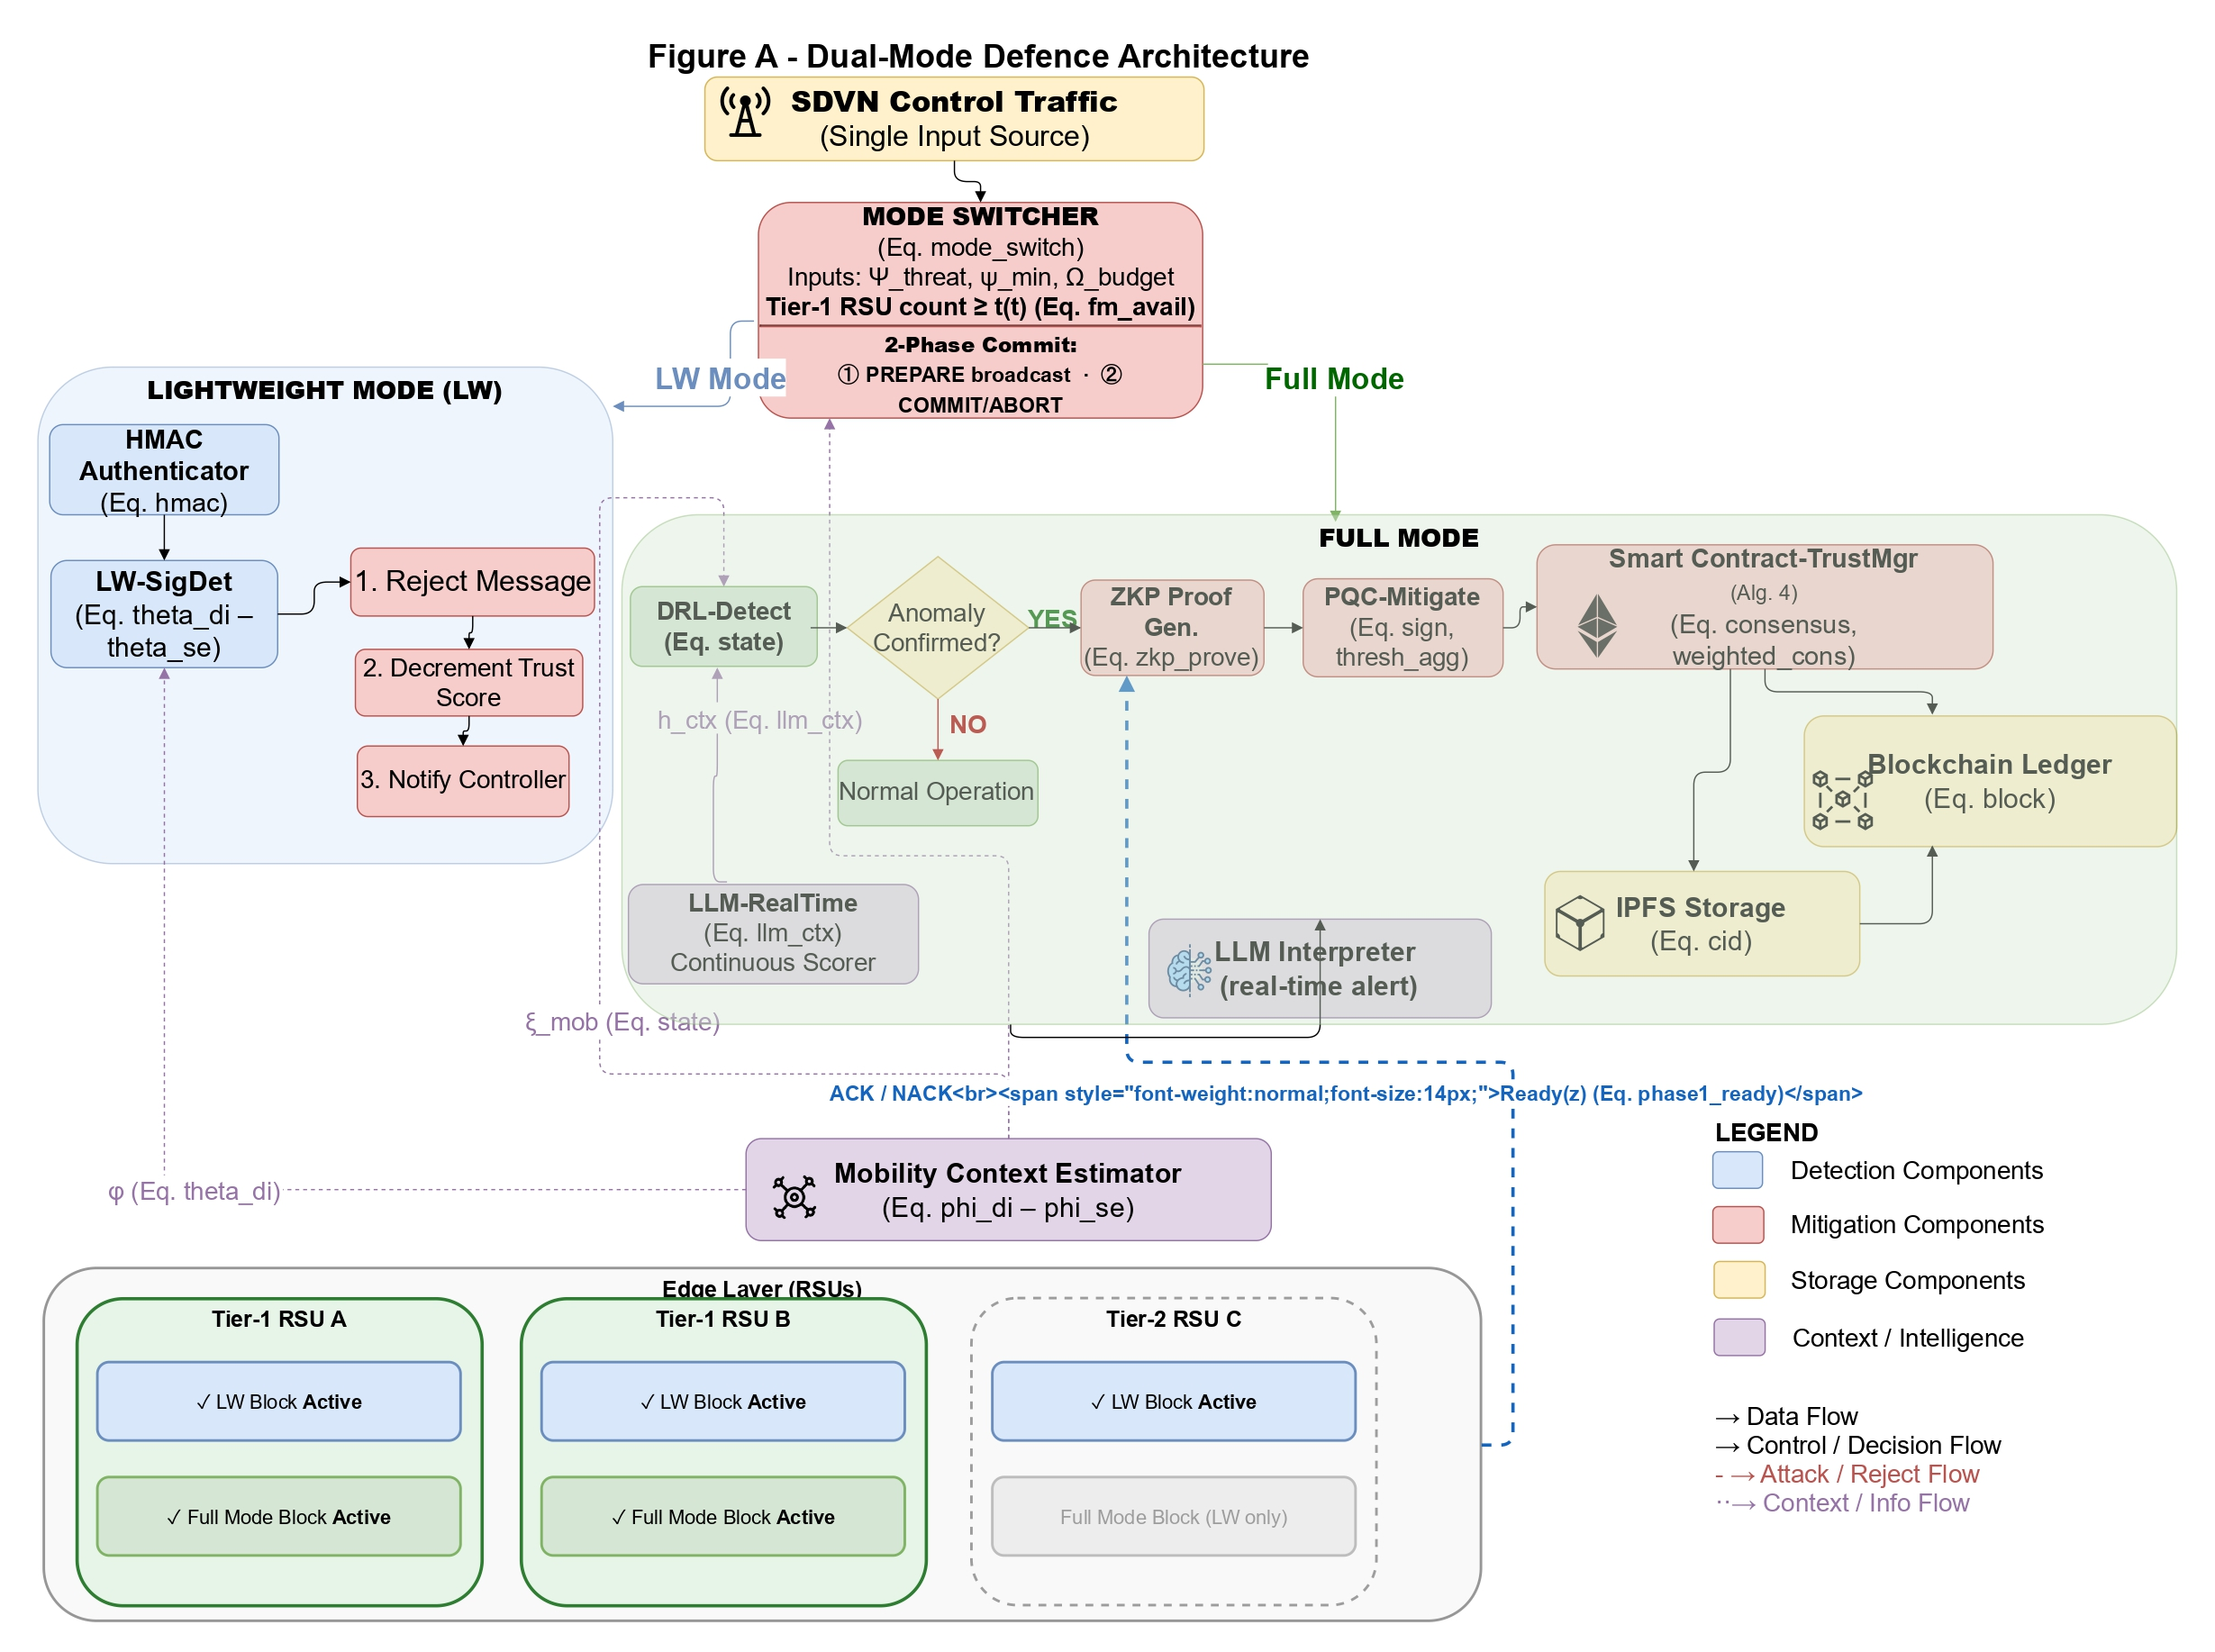
\includegraphics[width=\linewidth]{Progress_Works/DMAP_SDVN/Figure_A_Correct.jpg}
\caption{DMAP-SDVN dual-mode defence architecture.}
\label{fig:dual_mode}
\end{figure}
\FloatBarrier
% ====== END FIGURE A ======


As shown in Figure~\ref{fig:dual_mode}, all incoming traffic
enters the Mode Switcher which evaluates the threat score
$\Psi_{\mathrm{threat}}$ and resource budget
$\Omega_{\mathrm{budget}}$ to route traffic to either the LW
lane for lightweight rule-based detection or the Full Mode
lane for DRL, blockchain, PQC, and LLM-assisted detection and
mitigation. Both lanes share the Mobility Context Estimator
that feeds amplification factors $\Phi_{\mathrm{DI}}$ through
$\Phi_{\mathrm{SE}}$ to ensure mobility-aware decisions.


\begin{comment}
...
\end{comment}

The role of cryptographic mechanisms differs across attack variants and
determines their placement in the framework. For the \emph{timing
side-channel attack}, channel encryption directly prevents passive
observation of response times; accordingly, encrypted control-plane
channels with mutual authentication are applied \emph{pre-detection}
as primary preventive mitigation. For \emph{delay injection} and
\emph{synchronisation exploits}, PQC-signed timestamps and freshness
tokens enable accurate timing-baseline establishment but cannot prevent
a compromised RSU from withholding packets; PQC signing is therefore
applied \emph{pre-detection} to improve DRL detection accuracy, while
smart-contract-enforced trust revocation and path rerouting constitute
\emph{post-detection} mitigation. For \emph{race-condition exploitation},
conflicting link-state events can each carry valid signatures; cryptography
alone cannot resolve contradictions, so smart-contract atomic update
enforcement and DRL-guided event quarantine serve exclusively as
\emph{post-detection} mitigation. This analysis motivates the dual-role
cryptographic design in Section~\ref{sec:pqc}.


\begin{comment}
Algorithm~\ref{alg:di} presents the full detection and
mitigation cycle for Delay Injection attacks.

\begin{algorithm}[H]
\caption{Delay Injection Detection and Mitigation
(\texttt{DI-Defend})}
\label{alg:di}
\begin{algorithmic}[1]
\small
\Procedure{\texttt{DI-Defend}}
  {$m,\hat{v}_k,\mathrm{mode},\pi_\theta,\mathrm{sk}_{\mathrm{ctrl}}$}
  \State \textbf{ Authentication }
  \State Verify $\tau_{\mathrm{HMAC}}(m)$~\eqref{eq:hmac};
    \textbf{if} invalid \textbf{then return} \textsc{Reject}
  \State Verify $\mathrm{ML\text{-}DSA.Verify}
    (\mathrm{pk}_{\mathrm{ctrl}},m,\sigma_m)$~\eqref{eq:verify};
    \textbf{if} invalid \textbf{then return} \textsc{Reject}
  \State Check nonce freshness and TTL;
    \textbf{if} expired \textbf{then return} \textsc{Reject}
  \State \textbf{ Delay Detection }
  \State $\Delta\tau \gets T_{\mathrm{obs}}^m - T_{\mathrm{exp}}^m$
    \Comment{from~\eqref{eq:expected}}
  \State $\theta_{DI} \gets \tau_{\mathrm{TTL}}
    (1+\alpha_{DI}\hat{v}_k/v_{\max})-\epsilon_0$
    \Comment{from~\eqref{eq:theta_di}}
  \State $S_{DI} \gets \mathbb{1}[\Delta\tau > \theta_{DI}]$
    \Comment{from~\eqref{eq:sig_di}}
  \If{$S_{DI}=0$}
    \State Accept $m$; update $\psi_r \uparrow$~\eqref{eq:trust_update}
    \State \textbf{return} \textsc{Benign}
  \EndIf
  \State \textbf{ Mode-Dependent Mitigation }
  \If{$\mathrm{mode} = \mathrm{LW}$}
    \State Discard $m$; log locally;
      decrement $\psi_r \gets \psi_r - \Delta_{\mathrm{penalty}}$
    \State \textbf{return} $(\textsc{Attack},\mathrm{DI},\Delta\tau)$
  \EndIf
  \State \textbf{ Full Mode: DRL + Blockchain }
  \State $\pi_{\mathrm{ZKP}} \gets \mathrm{ZKProve}
    (T_{\mathrm{obs}}^m, \theta_{DI})$~\eqref{eq:zkp_prove}
  \State $C_m \gets \mathrm{Hash}
    (m\|\Delta\tau\|\pi_{\mathrm{ZKP}}\|\sigma_m)$
    \Comment{from~\eqref{eq:commitment}}
  \State $\mathrm{CID} \gets \mathrm{IPFS\_Store}(C_m)$
    \Comment{from~\eqref{eq:cid}}
  \State \texttt{SmartContract.SubmitTimingProof}
    $(r,C_m,\sigma_r)$
  \State $\mathbf{s}_t \gets \texttt{BuildState}
    (\Delta\tau,\boldsymbol{\psi},\boldsymbol{\xi},
    \mathbf{h}^{\mathrm{ctx}})$~\eqref{eq:state}
  \State $a_t \gets \pi_\theta(\mathbf{s}_t)$
    \Comment{from~\eqref{eq:actions}}
  \If{$a_t \in \{a_2^{\mathrm{isolate}},a_3^{\mathrm{reroute}}\}$}
    \State \texttt{PQC-Mitigate}$(r,\mathrm{DI},
      \mathrm{sk}_{\mathrm{ctrl}})$
  \EndIf
  \State \textbf{return} $(\textsc{Attack},\mathrm{DI},
    a_t,\mathrm{CID})$
\EndProcedure
\end{algorithmic}
\end{algorithm}

As shown in Algorithm~\ref{alg:di}, the procedure begins
with HMAC and ML-DSA authentication before any timing
analysis, ensuring unsigned or replayed messages are
rejected immediately. In LW mode, a confirmed delay
deviation above $\theta_{\mathrm{DI}}$ causes local
message rejection and trust decrement with no blockchain
overhead. In Full mode, a ZKP proof is generated, the
commitment is anchored to IPFS, and the DRL agent selects
an action from isolate, reroute, or strict verification.

\paragraph{Mitigation Strategy Using Deep Reinforcement Learning}
To mitigate race-condition exploitation attacks, we propose a DRL-based defense mechanism that treats attack detection and response as a real-time control problem. The DRL model learns optimal policies for identifying suspicious event timing patterns and applying appropriate mitigation actions to prevent inconsistent flow rules from being implemented.
\end{comment}
%-----------------------------------------------------

\subsubsection{Attack Signature Identification and Lightweight Detection}
\label{sec:signatures}

Each timing attack variant is characterised by a measurable
\emph{attack signature} — a distinguishing temporal or statistical
observable that separates malicious from benign behaviour. These
signatures form the basis of the Lightweight (LW) detection mode and
also seed the DRL state vector in the Full mode.


\begin{comment}
    
\textbf{Delay Injection Signature (DI).}
The attack produces a systematic positive temporal deviation exceeding
a mobility-adapted threshold. Define the signature indicator as
\begin{equation}
S_{\mathrm{DI}}(m) =
  \begin{cases}
    1 & \text{if } T_{\mathrm{obs}}^{m} - T_{\mathrm{exp}}^{m}
        > \theta_{\mathrm{DI}}(\hat{v}_k,\hat{H}) \\
    0 & \text{otherwise,}
  \end{cases}
\label{eq:sig_di}
\end{equation}
where $T_{\mathrm{obs}}^{m}$ is the observed arrival time,
$T_{\mathrm{exp}}^{m}$ is derived from~\eqref{eq:expected}, and the
adaptive threshold is
\begin{equation}
\theta_{\mathrm{DI}}(\hat{v}_k,\hat{H}) =
  \tau_{\mathrm{TTL}}\!\left(1 +
  \alpha_{\mathrm{DI}}\,\frac{\hat{v}_k}{v_{\max}}\right) - \epsilon_0,
\label{eq:theta_di}
\end{equation}
adjusting for estimated vehicle speed $\hat{v}_k$ and channel
quality $\hat{H}$, preventing false positives under high-mobility
legitimate topology changes.
\end{comment}

\textbf{Delay Injection Signature (DI).}
The attack produces a systematic positive temporal deviation
exceeding a mobility-adapted threshold. The delay injection
signature indicator is defined in Equation~\eqref{eq:sig_di}.
\begin{equation}
S_{\mathrm{DI}}(m) =
  \begin{cases}
    1 & \text{if } T_{\mathrm{obs}}^{m} - T_{\mathrm{exp}}^{m}
        > \theta_{\mathrm{DI}}(\hat{v}_k,\hat{H}) \\
    0 & \text{otherwise,}
  \end{cases}
\label{eq:sig_di}
\end{equation}
As shown in Equation~\eqref{eq:sig_di}, $T_{\mathrm{obs}}^{m}$
is the observed arrival time and $T_{\mathrm{exp}}^{m}$ is derived
from~\eqref{eq:expected}. The indicator fires when the temporal
deviation exceeds the mobility-adapted threshold
$\theta_{\mathrm{DI}}$, which is defined in
Equation~\eqref{eq:theta_di}.
\begin{equation}
\theta_{\mathrm{DI}}(\hat{v}_k,\hat{H}) =
  \tau_{\mathrm{TTL}}\!\left(1 +
  \alpha_{\mathrm{DI}}\,\frac{\hat{v}_k}{v_{\max}}\right) - \epsilon_0,
\label{eq:theta_di}
\end{equation}
As shown in Equation~\eqref{eq:theta_di}, the threshold scales
with estimated vehicle speed $\hat{v}_k$ and channel quality
$\hat{H}$, preventing false positives under high-mobility
legitimate topology changes.

\begin{comment}
\textbf{Race Condition Signature (RC).}
The attack is characterised by semantically contradictory link-state
events from the same RSU within a critical temporal window:
\begin{equation}
S_{\mathrm{RC}}(e_1, e_2) =
  \mathbb{1}\!\left[\mathcal{C}(e_1,e_2){=}{-}1\right]
  \cdot\mathbb{1}\!\left[|t_{e_1}{-}t_{e_2}| < \epsilon_{\mathrm{RC}}\right]
  \cdot\mathbb{1}\!\left[\mathrm{src}(e_1){=}\mathrm{src}(e_2)\right],
\label{eq:sig_rc}
\end{equation}
where $\mathcal{C}(e_1,e_2)\in\{-1,0,1\}$ is a conflict indicator
($-1$ for contradictory events such as simultaneous Link-Up and
Link-Down), $\epsilon_{\mathrm{RC}}$ is the race window, and the
third predicate requires the same source RSU to rule out legitimate
multi-RSU disagreement.
\end{comment}


\textbf{Race Condition Signature (RC).}
The attack is characterised by semantically contradictory
link-state events from the same RSU within a critical temporal
window. The race condition signature indicator is defined in
Equation~\eqref{eq:sig_rc}.
\begin{equation}
S_{\mathrm{RC}}(e_1, e_2) =
  \mathbb{1}\!\left[\mathcal{C}(e_1,e_2){=}{-}1\right]
  \cdot\mathbb{1}\!\left[|t_{e_1}{-}t_{e_2}| < \epsilon_{\mathrm{RC}}\right]
  \cdot\mathbb{1}\!\left[\mathrm{src}(e_1){=}\mathrm{src}(e_2)\right],
\label{eq:sig_rc}
\end{equation}
As shown in Equation~\eqref{eq:sig_rc},
$\mathcal{C}(e_1,e_2)\in\{-1,0,1\}$ is a conflict indicator
($-1$ for contradictory events such as simultaneous Link-Up
and Link-Down), $\epsilon_{\mathrm{RC}}$ is the race window,
and the third predicate requires the same source RSU to rule
out legitimate multi-RSU disagreement. All three conditions
must hold simultaneously for the signature to fire.


\begin{comment}
\textbf{Timing Side-Channel Signature (SC).}
The attack manifests as an anomalously strong statistical correlation
between control-plane response times and discrete network events,
combined with unnaturally low timing jitter:
\begin{equation}
S_{\mathrm{SC}}(\mathbf{T}_{1:n}) =
  \mathbb{1}\!\left[\rho(\mathbf{T}_{1:n},\mathbf{E}_{1:n})
    > \rho_{th}\right]
  \cdot
  \mathbb{1}\!\left[\hat{\sigma}_{\mathrm{timing}}
    < \theta_{\mathrm{noise}}\right],
\label{eq:sig_sc}
\end{equation}
where $\rho(\cdot,\cdot)$ is the Pearson correlation between the
observed timing sequence $\mathbf{T}_{1:n}$ and network event
indicators $\mathbf{E}_{1:n}$, $\rho_{th}$ is the suspicious
correlation threshold, and $\hat{\sigma}_{\mathrm{timing}} 
\theta_{\mathrm{noise}}$ indicates the pattern is too regular to
arise from natural channel jitter.
\end{comment}


\textbf{Timing Side-Channel Signature (SC).}
The attack manifests as an anomalously strong statistical
correlation between control-plane response times and discrete
network events, combined with unnaturally low timing jitter.
The timing side-channel signature indicator is defined in
Equation~\eqref{eq:sig_sc}.
\begin{equation}
S_{\mathrm{SC}}(\mathbf{T}_{1:n}) =
  \mathbb{1}\!\left[\rho(\mathbf{T}_{1:n},\mathbf{E}_{1:n})
    > \rho_{th}\right]
  \cdot
  \mathbb{1}\!\left[\hat{\sigma}_{\mathrm{timing}}
    < \theta_{\mathrm{noise}}\right],
\label{eq:sig_sc}
\end{equation}
As shown in Equation~\eqref{eq:sig_sc}, $\rho(\cdot,\cdot)$
is the Pearson correlation between the observed timing sequence
$\mathbf{T}_{1:n}$ and network event indicators
$\mathbf{E}_{1:n}$, and $\rho_{th}$ is the suspicious
correlation threshold. The second predicate checks that
$\hat{\sigma}_{\mathrm{timing}} < \theta_{\mathrm{noise}}$,
indicating the timing pattern is too regular to arise from
natural channel jitter. Both conditions must hold to reduce
false positives from congestion-induced correlation.

\begin{comment}
\textbf{Synchronisation Exploit Signature (SE).}
The attack produces detectable beacon gaps combined with
anomalously high inter-arrival variance:
\begin{equation}
S_{\mathrm{SE}}(\mathbf{b}_{1:n}) =
  \mathbb{1}\!\left[\exists\,k:\;b_k > \tfrac{2}{f_{\mathrm{beacon}}}
  \right]
  \cdot
  \mathbb{1}\!\left[\tfrac{1}{n}
    \sum_{i=1}^{n}(b_i-\bar{b})^2 > \theta_{\mathrm{SE}}^2\right],
\label{eq:sig_se}
\end{equation}
where $\mathbf{b}_{1:n}$ are beacon inter-arrival times; the first
predicate detects a missing beacon (gap exceeding two beacon periods)
and the second detects high temporal variance across the window.
\end{comment}

\textbf{Synchronisation Exploit Signature (SE).}
The attack produces detectable beacon gaps combined with
anomalously high inter-arrival variance. The synchronisation
exploit signature indicator is defined in
Equation~\eqref{eq:sig_se}.
\begin{equation}
S_{\mathrm{SE}}(\mathbf{b}_{1:n}) =
  \mathbb{1}\!\left[\exists\,k:\;b_k > \tfrac{2}{f_{\mathrm{beacon}}}
  \right]
  \cdot
  \mathbb{1}\!\left[\tfrac{1}{n}
    \sum_{i=1}^{n}(b_i-\bar{b})^2 > \theta_{\mathrm{SE}}^2\right],
\label{eq:sig_se}
\end{equation}
As shown in Equation~\eqref{eq:sig_se}, $\mathbf{b}_{1:n}$
are beacon inter-arrival times. The first predicate detects a
missing beacon when the gap exceeds two beacon periods
$2/f_{\mathrm{beacon}}$, and the second detects high temporal
variance across the observation window. Both must be satisfied
simultaneously to distinguish an attack from transient channel
loss.


\begin{comment}
In LW mode, the HMAC-based lightweight authentication tag for each
control-plane message $m$ is computed as
\begin{equation}
\tau_{\mathrm{HMAC}}(m) =
  \mathrm{HMAC\text{-}SHA256}\!\left(K_s,\;
  m \,\|\, T_{\mathrm{obs}}^{m} \,\|\, \mathrm{seq}(m)\right),
\label{eq:hmac}
\end{equation}
where $K_s$ is the shared session key and $\mathrm{seq}(m)$ is a
monotonically increasing sequence number preventing replay. Any message
failing HMAC verification is immediately discarded before signature
evaluation.
\end{comment}
In LW mode, the HMAC-based lightweight authentication tag for
each control-plane message $m$ is computed as given in
Equation~\eqref{eq:hmac}.
\begin{equation}
\tau_{\mathrm{HMAC}}(m) =
  \mathrm{HMAC\text{-}SHA256}\!\left(K_s,\;
  m \,\|\, T_{\mathrm{obs}}^{m} \,\|\, \mathrm{seq}(m)\right),
\label{eq:hmac}
\end{equation}
As shown in Equation~\eqref{eq:hmac}, $K_s$ is the shared
session key and $\mathrm{seq}(m)$ is a monotonically increasing
sequence number preventing replay attacks. Any message failing
HMAC verification is immediately discarded before signature
evaluation, ensuring unauthenticated messages never reach the
attack detection stage.


Algorithm~\ref{alg:lw} presents the complete Lightweight
Signature Detection procedure that combines all four
signature checks into a single $O(1)$-per-message function
executed at each RSU.

\begin{algorithm}[H]
\caption{Lightweight Signature Detection (\texttt{LW-SigDet})}
\label{alg:lw}
\begin{algorithmic}[1]
\small
\Procedure{\texttt{LW-SigDet}}{$m,\mathbf{b}_{1:n},\mathcal{E},\hat{v}_k$}
  \State Verify $\tau_{\mathrm{HMAC}}(m)$; \textbf{if} invalid
    \textbf{then return} \textsc{Reject}
  \State $\Delta\tau \gets T_{\mathrm{obs}}^m - T_{\mathrm{exp}}^m$
  \State $\theta_{DI} \gets \tau_{\mathrm{TTL}}
    (1+\alpha_{DI}\hat{v}_k/v_{\max})-\epsilon_0$
  \If{$\Delta\tau > \theta_{DI}$}
    \State \textbf{return} $(\textsc{Attack},\,\mathrm{DI},\,\Delta\tau)$
  \EndIf
  \For{each pair $(e_1,e_2)\in\mathcal{E}$ from same RSU}
    \If{$\mathcal{C}(e_1,e_2)=-1$
        \textbf{and} $|t_{e_1}-t_{e_2}|<\epsilon_{RC}$}
      \State \textbf{return} $(\textsc{Attack},\,\mathrm{RC},\,e_1,e_2)$
    \EndIf
  \EndFor
  \State $\hat{\rho} \gets
    \texttt{PearsonCorr}(\mathbf{T}_{1:n},\mathbf{E}_{1:n})$
  \If{$\hat{\rho}>\rho_{th}$
      \textbf{and} $\hat{\sigma}_{\mathrm{timing}}<\theta_{\mathrm{noise}}$}
    \State \textbf{return} $(\textsc{Attack},\,\mathrm{SC},\,\hat{\rho})$
  \EndIf
  \State $\mathrm{gap}\gets
    \exists\,k:\,b_k > 2/f_{\mathrm{beacon}}$
  \State $\mathrm{var}\gets
    \frac{1}{n}\sum_{i=1}^{n}(b_i-\bar{b})^2$
  \If{$\mathrm{gap}$ \textbf{and}
      $\mathrm{var}>\theta_{\mathrm{SE}}^2$}
    \State \textbf{return}
      $(\textsc{Attack},\,\mathrm{SE},\,\mathrm{var})$
  \EndIf
  \State \textbf{return} $\perp$
\EndProcedure
\end{algorithmic}
\end{algorithm}

As shown in Algorithm~\ref{alg:lw}, the procedure first
verifies the HMAC tag and rejects unauthenticated messages
immediately. It then evaluates the four signature checks in
sequence  DI threshold comparison, RC conflict pair
detection, SC Pearson correlation check, and SE beacon gap
variance check  returning the first detected attack type
or $\perp$ if all checks pass. The sequential order
prioritises the lowest-cost checks first, keeping
per-message overhead at $O(1)$.




\begin{comment}
...
\end{comment}

% \subsection{Per-Variant Detection and Mitigation Algorithms}
% Algorithm~\ref{alg:di} covers the full detection and mitigation
% cycle for delay injection attacks, operating in both LW and Full
% modes. In LW mode, HMAC verification and threshold comparison
% provide immediate rejection; in Full mode, the DRL agent and
% smart contract provide adaptive enforcement.

% \begin{algorithm}[H]
% \caption{Delay Injection Detection and Mitigation
% (\texttt{DI-Defend})}
% \label{alg:di}
% \begin{algorithmic}[1]
% \small
% \Procedure{\texttt{DI-Defend}}
%   {$m,\hat{v}_k,\mathrm{mode},\pi_\theta,\mathrm{sk}_{\mathrm{ctrl}}$}
%   \State \textbf{--- Authentication ---}
%   \State Verify $\tau_{\mathrm{HMAC}}(m)$~\eqref{eq:hmac};
%     \textbf{if} invalid \textbf{then return} \textsc{Reject}
%   \State Verify $\mathrm{ML\text{-}DSA.Verify}
%     (\mathrm{pk}_{\mathrm{ctrl}},m,\sigma_m)$~\eqref{eq:verify};
%     \textbf{if} invalid \textbf{then return} \textsc{Reject}
%   \State Check nonce freshness and TTL;
%     \textbf{if} expired \textbf{then return} \textsc{Reject}
%   \State \textbf{--- Delay Detection ---}
%   \State $\Delta\tau \gets T_{\mathrm{obs}}^m - T_{\mathrm{exp}}^m$
%     \Comment{from~\eqref{eq:expected}}
%   \State $\theta_{DI} \gets \tau_{\mathrm{TTL}}
%     (1+\alpha_{DI}\hat{v}_k/v_{\max})-\epsilon_0$
%     \Comment{from~\eqref{eq:theta_di}}
%   \State $S_{DI} \gets \mathbb{1}[\Delta\tau > \theta_{DI}]$
%     \Comment{from~\eqref{eq:sig_di}}
%   \If{$S_{DI}=0$}
%     \State Accept $m$; update $\psi_r \uparrow$~\eqref{eq:trust_update}
%     \State \textbf{return} \textsc{Benign}
%   \EndIf
%   \State \textbf{--- Mode-Dependent Mitigation ---}
%   \If{$\mathrm{mode} = \mathrm{LW}$}
%     \State Discard $m$; log locally;
%       decrement $\psi_r \gets \psi_r - \Delta_{\mathrm{penalty}}$
%     \State \textbf{return} $(\textsc{Attack},\mathrm{DI},\Delta\tau)$
%   \EndIf
%   \State \textbf{--- Full Mode: DRL + Blockchain ---}
%   \State $\pi_{\mathrm{ZKP}} \gets \mathrm{ZKProve}
%     (T_{\mathrm{obs}}^m, \theta_{DI})$~\eqref{eq:zkp_prove}
%   \State $C_m \gets \mathrm{Hash}
%     (m\|\Delta\tau\|\pi_{\mathrm{ZKP}}\|\sigma_m)$
%     \Comment{from~\eqref{eq:commitment}}
%   \State $\mathrm{CID} \gets \mathrm{IPFS\_Store}(C_m)$
%     \Comment{from~\eqref{eq:cid}}
%   \State \texttt{SmartContract.SubmitTimingProof}
%     $(r,C_m,\sigma_r)$~\Comment{Alg.~\ref{alg:sc}}
%   \State $\mathbf{s}_t \gets \texttt{BuildState}
%     (\Delta\tau,\boldsymbol{\psi},\boldsymbol{\xi},
%     \mathbf{h}^{\mathrm{ctx}})$~\eqref{eq:state}
%   \State $a_t \gets \pi_\theta(\mathbf{s}_t)$
%     \Comment{from~\eqref{eq:actions}}
%   \If{$a_t \in \{a_2^{\mathrm{isolate}},a_3^{\mathrm{reroute}}\}$}
%     \State \texttt{PQC-Mitigate}$(r,\mathrm{DI},
%       \mathrm{sk}_{\mathrm{ctrl}})$~\Comment{Alg.~\ref{alg:pqc}}
%   \EndIf
%   \State \textbf{return} $(\textsc{Attack},\mathrm{DI},
%     a_t,\mathrm{CID})$
% \EndProcedure
% \end{algorithmic}
% \end{algorithm}


% Algorithm~\ref{alg:rc} handles race condition exploitation
% by detecting contradictory event pairs and enforcing atomic
% flow-rule update semantics via smart contracts in Full mode.

% \begin{algorithm}[H]
% \caption{Race Condition Detection and Mitigation
% (\texttt{RC-Defend})}
% \label{alg:rc}
% \begin{algorithmic}[1]
% \small
% \Procedure{\texttt{RC-Defend}}
%   {$e_{\mathrm{new}},\mathcal{Q},\mathrm{mode},
%   \pi_\theta,\mathrm{sk}_{\mathrm{ctrl}}$}
%   \State \textbf{--- Event Queue Inspection ---}
%   \State Append $e_{\mathrm{new}}$ to event queue $\mathcal{Q}$
%   \For{each $e_{\mathrm{prev}} \in \mathcal{Q}$
%     from $\mathrm{src}(e_{\mathrm{new}})$}
%     \State $\mathcal{C} \gets
%       \mathrm{ConflictCheck}(e_{\mathrm{prev}},e_{\mathrm{new}})$
%       \Comment{from~\eqref{eq:sig_rc}}
%     \State $\Delta t \gets |t_{e_{\mathrm{new}}}
%       - t_{e_{\mathrm{prev}}}|$
%     \If{$\mathcal{C}=-1$
%         \textbf{and} $\Delta t < \epsilon_{RC}$}
%       \State $S_{RC} \gets 1$; break
%     \EndIf
%   \EndFor
%   \If{$S_{RC}=0$}
%     \State Process $e_{\mathrm{new}}$ normally;
%       generate Flow-Mod
%     \State \textbf{return} \textsc{Benign}
%   \EndIf
%   \State \textbf{--- Mode-Dependent Mitigation ---}
%   \If{$\mathrm{mode} = \mathrm{LW}$}
%     \State Hold both conflicting Flow-Mods;
%       request re-report from RSU
%     \State Decrement
%       $\psi_r \gets \psi_r - \Delta_{\mathrm{penalty}}$
%     \State \textbf{return}
%       $(\textsc{Attack},\mathrm{RC},e_{\mathrm{prev}},
%       e_{\mathrm{new}})$
%   \EndIf
%   \State \textbf{--- Full Mode: Atomic Enforcement ---}
%   \State $\mathbf{s}_t \gets \texttt{BuildState}
%     (\Delta\tau^{RC},\boldsymbol{\psi},\boldsymbol{\xi},
%     \mathbf{h}^{\mathrm{ctx}})$~\eqref{eq:state}
%   \State $a_t \gets \pi_\theta(\mathbf{s}_t)$
%   \If{$a_t = a_1^{\mathrm{verify}}$}
%     \State Query $\geq t$ neighbouring RSUs for
%       link-state consensus
%     \State Accept majority-consistent event;
%       discard outlier
%   \ElsIf{$a_t \in
%     \{a_2^{\mathrm{isolate}},a_4^{\mathrm{strict}}\}$}
%     \State \texttt{SmartContract.EnforceAtomicUpdate}
%       $(r,e_{\mathrm{prev}},e_{\mathrm{new}})$
%     \State \texttt{PQC-Mitigate}$(r,\mathrm{RC},
%       \mathrm{sk}_{\mathrm{ctrl}})$~\Comment{Alg.~\ref{alg:pqc}}
%   \EndIf
%   \State $C_{RC} \gets \mathrm{Hash}
%     (e_{\mathrm{prev}}\|e_{\mathrm{new}}\|\Delta t)$
%   \State $\mathrm{CID} \gets \mathrm{IPFS\_Store}(C_{RC})$
%   \State \textbf{return}
%     $(\textsc{Attack},\mathrm{RC},a_t,\mathrm{CID})$
% \EndProcedure
% \end{algorithmic}
% \end{algorithm}


% Algorithm~\ref{alg:sc_def} addresses timing side-channel
% attacks by computing correlation-based signatures over a
% sliding observation window and applying channel obfuscation
% as the primary mitigation in both modes.

% \begin{algorithm}[H]
% \caption{Timing Side-Channel Detection and Mitigation
% (\texttt{SC-Defend})}
% \label{alg:sc_def}
% \begin{algorithmic}[1]
% \small
% \Procedure{\texttt{SC-Defend}}
%   {$\mathbf{T}_{1:n},\mathbf{E}_{1:n},\mathrm{mode},
%   \pi_\theta,\mathrm{sk}_{\mathrm{ctrl}}$}
%   \State \textbf{--- Passive Observation Detection ---}
%   \State $\hat{\rho} \gets
%     \mathrm{PearsonCorr}(\mathbf{T}_{1:n},\mathbf{E}_{1:n})$
%   \State $\hat{\sigma}_{\mathrm{timing}} \gets
%     \mathrm{std}(\mathbf{T}_{1:n})$
%   \State $S_{SC} \gets
%     \mathbb{1}[\hat{\rho}>\rho_{th}]
%     \cdot\mathbb{1}
%     [\hat{\sigma}_{\mathrm{timing}}<\theta_{\mathrm{noise}}]$
%     \Comment{from~\eqref{eq:sig_sc}}
%   \If{$S_{SC}=0$}
%     \State Continue normal operation
%     \State \textbf{return} \textsc{Benign}
%   \EndIf
%   \State \textbf{--- Immediate Preventive Action
%     (both modes) ---}
%   \State Inject calibrated timing noise
%     $\eta \sim \mathcal{U}(0,\epsilon_{\mathrm{noise}})$
%     into response times
%   \State Enforce encrypted channels with mutual
%     authentication on all links from suspected observer
%   \State \textbf{--- Mode-Dependent Mitigation ---}
%   \If{$\mathrm{mode} = \mathrm{LW}$}
%     \State Log $(\hat{\rho},\hat{\sigma})$ locally;
%       flag RSU for monitoring
%     \State \textbf{return}
%       $(\textsc{Attack},\mathrm{SC},\hat{\rho})$
%   \EndIf
%   \State \textbf{--- Full Mode: ZKP + DRL ---}
%   \State Switch all RSU timing attestations to
%     ZKP mode~\eqref{eq:zkp_prove}
%     \Comment{prevents exact time leakage}
%   \State $\mathbf{s}_t \gets \texttt{BuildState}
%     (\hat{\rho},\boldsymbol{\psi},\boldsymbol{\xi},
%     \mathbf{h}^{\mathrm{ctx}})$~\eqref{eq:state}
%   \State $a_t \gets \pi_\theta(\mathbf{s}_t)$
%   \If{$a_t \in
%     \{a_2^{\mathrm{isolate}},a_4^{\mathrm{strict}}\}$}
%     \State \texttt{PQC-Mitigate}$(r,\mathrm{SC},
%       \mathrm{sk}_{\mathrm{ctrl}})$~\Comment{Alg.~\ref{alg:pqc}}
%   \EndIf
%   \State $C_{SC} \gets \mathrm{Hash}
%     (\hat{\rho}\|\hat{\sigma}\|\mathbf{T}_{1:n})$
%   \State $\mathrm{CID} \gets \mathrm{IPFS\_Store}(C_{SC})$
%   \State \textbf{return}
%     $(\textsc{Attack},\mathrm{SC},a_t,\mathrm{CID})$
% \EndProcedure
% \end{algorithmic}
% \end{algorithm}


% Algorithm~\ref{alg:se} addresses synchronisation exploits
% by monitoring beacon inter-arrival patterns and handover
% report timing differentials, with mobility-aware thresholds
% to avoid false positives during legitimate handovers.

% \begin{algorithm}[H]
% \caption{Synchronisation Exploit Detection and Mitigation
% (\texttt{SE-Defend})}
% \label{alg:se}
% \begin{algorithmic}[1]
% \small
% \Procedure{\texttt{SE-Defend}}
%   {$\mathbf{b}_{1:n},\mathbf{R}_t,\mathrm{mode},
%   \pi_\theta,\mathrm{sk}_{\mathrm{ctrl}}$}
%   \State \textbf{--- Beacon Synchronisation Check ---}
%   \State $\mathrm{gap} \gets
%     \exists\,k:\;b_k > 2/f_{\mathrm{beacon}}$
%   \State $\mathrm{var} \gets
%     \frac{1}{n}\sum_{i=1}^{n}(b_i-\bar{b})^2$
%   \State $S_{SE}^{\mathrm{beacon}} \gets
%     \mathbb{1}[\mathrm{gap}]
%     \cdot\mathbb{1}[\mathrm{var}>\theta_{SE}^2]$
%     \Comment{from~\eqref{eq:sig_se}}
%   \State \textbf{--- Handover Report Timing Check ---}
%   \State $\Delta\tau_{\mathrm{HO}} \gets
%     |T_{\mathrm{report}}^{r_A} - T_{\mathrm{report}}^{r_B}|$
%     \Comment{differential between RSU reports}
%   \State $S_{SE}^{\mathrm{HO}} \gets
%     \mathbb{1}[\Delta\tau_{\mathrm{HO}} >
%     \theta_{\mathrm{HO}}(\hat{v}_k)]$
%     \Comment{mobility-adapted threshold}
%   \State $S_{SE} \gets
%     S_{SE}^{\mathrm{beacon}} \vee S_{SE}^{\mathrm{HO}}$
%   \If{$S_{SE}=0$}
%     \State Proceed with handover decision;
%       update $\psi_r \uparrow$
%     \State \textbf{return} \textsc{Benign}
%   \EndIf
%   \State \textbf{--- Mode-Dependent Mitigation ---}
%   \If{$\mathrm{mode} = \mathrm{LW}$}
%     \State Apply hysteresis: require 3 consecutive
%       valid beacons before handover commit
%     \State Decrement
%       $\psi_r \gets \psi_r - \Delta_{\mathrm{penalty}}$
%     \State \textbf{return}
%       $(\textsc{Attack},\mathrm{SE},\mathrm{var},
%       \Delta\tau_{\mathrm{HO}})$
%   \EndIf
%   \State \textbf{--- Full Mode: Spatio-Temporal
%     Validation + DRL ---}
%   \State Validate vehicle trajectory plausibility:
%     $\mathbf{p}_k(t)$ vs historical $\boldsymbol{\xi}_k$
%   \State Request threshold-signed corroboration from
%     $\geq t$ RSUs~\eqref{eq:thresh_agg}
%   \State $\mathbf{s}_t \gets \texttt{BuildState}
%     (\Delta b,\boldsymbol{\psi},\boldsymbol{\xi},
%     \mathbf{h}^{\mathrm{ctx}})$~\eqref{eq:state}
%   \State $a_t \gets \pi_\theta(\mathbf{s}_t)$
%   \If{$a_t \in
%     \{a_2^{\mathrm{isolate}},a_3^{\mathrm{reroute}}\}$}
%     \State \texttt{PQC-Mitigate}$(r,\mathrm{SE},
%       \mathrm{sk}_{\mathrm{ctrl}})$~\Comment{Alg.~\ref{alg:pqc}}
%   \EndIf
%   \State $S_{\mathrm{sync}}^{\mathrm{mob}} \gets$
%     compute~\eqref{eq:sync_mob}
%     \Comment{offline integrity record}
%   \State $C_{SE} \gets \mathrm{Hash}
%     (\mathrm{var}\|\Delta\tau_{\mathrm{HO}}\|
%     S_{\mathrm{sync}}^{\mathrm{mob}})$
%   \State $\mathrm{CID} \gets \mathrm{IPFS\_Store}(C_{SE})$
%   \State \textbf{return}
%     $(\textsc{Attack},\mathrm{SE},a_t,\mathrm{CID})$
% \EndProcedure
% \end{algorithmic}
% \end{algorithm}


\begin{comment}
...
\end{comment}


%-----------------------------------------------------



\subsubsection{DRL Detection Agent: MDP Formulation}
\label{sec:drl}


\begin{comment}
The timing-attack detection problem is formulated as a Markov Decision
Process (MDP) $(\mathcal{S},\mathcal{A},P,R,\gamma)$. The \emph{state vector} at epoch $t$ aggregates features for all four attack variants alongside mobility context and LLM-derived semantic intelligence:

%\begin{equation}
%\mathbf{s}_t = \bigl[
\end{comment}

The timing-attack detection problem is formulated as a Markov
Decision Process (MDP) $(\mathcal{S},\mathcal{A},P,R,\gamma)$.
The state vector at epoch $t$, which aggregates features for
all four attack variants alongside mobility context and
LLM-derived semantic intelligence, is given in
Equation~\eqref{eq:state}.
\begin{equation}
\mathbf{s}_t = \bigl[
  \underbrace{\Delta\tau_t^{\mathrm{DI}},\;
  \Delta\tau_t^{\mathrm{RC}},\;
  \rho_t^{\mathrm{SC}},\;
  \Delta b_t^{\mathrm{SE}}}_{\text{attack features}},\;
  \underbrace{\boldsymbol{\psi}_t^{\mathrm{trust}}}_{\text{trust}},\;
  \underbrace{\boldsymbol{\xi}_t^{\mathrm{mob}}}_{\text{mobility}},\;
  \underbrace{\mathbf{h}_t^{\mathrm{ctx}}}_{\text{LLM context}}
\bigr] \in \mathbb{R}^{d_s},
\label{eq:state}
\end{equation}

As shown in Equation~\eqref{eq:state}, the state vector
combines four attack-specific features, the RSU trust vector
$\boldsymbol{\psi}_t^{\mathrm{trust}}$, the mobility context
$\boldsymbol{\xi}_t^{\mathrm{mob}}$, and the LLM context
$\mathbf{h}_t^{\mathrm{ctx}}$ into a unified representation
of dimension $d_s$. The component $\mathbf{h}_t^{\mathrm{ctx}}$
is the LLM context vector~\eqref{eq:llm_ctx} carrying per-RSU
semantic anomaly scores $\lambda_t^r$ and attack-category
probability vectors $\hat{\mathbf{p}}_t^r$, enabling the DRL
agent to distinguish congestion-induced timing deviations from
adversarial attacks without relying solely on statistical
features.

\textbf{DRL State Feature Selection.}
Adapting the hybrid feature selection pipeline
of~\cite{satpathy2025cloud}, the raw feature pool
$\mathcal{F}_{\mathrm{raw}}$ for the DRL state
is reduced to a stable, interpretable subset
$\mathcal{F}^* \subseteq \mathcal{F}_{\mathrm{raw}}$ via a two-stage selection given in Equation~\eqref{eq:feat_sel}.
\begin{equation}
\mathcal{F}^* = \mathcal{F}_{\mathrm{Boruta}}
  \cap \mathcal{F}_{\mathrm{SHAP}},
\label{eq:feat_sel}
\end{equation}
As shown in Equation~\eqref{eq:feat_sel},
$\mathcal{F}_{\mathrm{Boruta}}$ retains features
confirmed significant by the Boruta wrapper test and
$\mathcal{F}_{\mathrm{SHAP}}$ retains the top-$k$
features ranked by SHAP importance scores
$\phi_j = \mathbb{E}[|Q(\mathbf{s},a) -
Q(\mathbf{s}_{-j},a)|]$ computed over the replay
buffer. The intersection ensures the DRL state
contains only features that are both statistically
significant and causally influential on the
Q-function, reducing state dimensionality $d_s$
and improving convergence under the non-stationary
timing distributions induced by vehicular mobility.


\begin{comment}
....
\end{comment}

\begin{comment}
The \emph{action space} is:
\begin{equation}
\mathcal{A} = \bigl\{
  a_0^{\mathrm{pass}},\;
  a_1^{\mathrm{verify}},\;
  a_2^{\mathrm{isolate}},\;
  a_3^{\mathrm{reroute}},\;
  a_4^{\mathrm{strict}}
\bigr\},
\label{eq:actions}
\end{equation}
corresponding respectively to: no action, cross-RSU re-verification
request, RSU quarantine, control-path rerouting, and strict
validation mode. 
\end{comment}

The action space available to the DRL agent is defined in
Equation~\eqref{eq:actions}.
\begin{equation}
\mathcal{A} = \bigl\{
  a_0^{\mathrm{pass}},\;
  a_1^{\mathrm{verify}},\;
  a_2^{\mathrm{isolate}},\;
  a_3^{\mathrm{reroute}},\;
  a_4^{\mathrm{strict}}
\bigr\},
\label{eq:actions}
\end{equation}
As shown in Equation~\eqref{eq:actions}, the five actions
correspond respectively to: no action
($a_0^{\mathrm{pass}}$), cross-RSU re-verification request
($a_1^{\mathrm{verify}}$), RSU quarantine
($a_2^{\mathrm{isolate}}$), control-path rerouting
($a_3^{\mathrm{reroute}}$), and strict validation mode
($a_4^{\mathrm{strict}}$).

\begin{comment}
The composite \emph{reward function} is:
\begin{equation}
R(\mathbf{s}_t,a_t) =
  \omega_1 R_{\mathrm{det}} +
  \omega_2 R_{\mathrm{mit}} -
  \omega_3 R_{\mathrm{lat}} -
  \omega_4 R_{\mathrm{fp}},
\label{eq:reward}
\end{equation}
where $\omega_1,\ldots,\omega_4$ are tunable weighting coefficients.
\end{comment}

The composite reward function is given in
Equation~\eqref{eq:reward}.
\begin{equation}
R(\mathbf{s}_t,a_t) =
  \omega_1 R_{\mathrm{det}} +
  \omega_2 R_{\mathrm{mit}} -
  \omega_3 R_{\mathrm{lat}} -
  \omega_4 R_{\mathrm{fp}},
\label{eq:reward}
\end{equation}
As shown in Equation~\eqref{eq:reward},
$\omega_1,\ldots,\omega_4$ are tunable weighting coefficients
that balance detection accuracy, mitigation speed, latency
penalty, and false-positive avoidance. The positive terms
reward correct detection and fast mitigation while the
negative terms penalise unnecessary delays and false alarms.


\begin{comment}
The \emph{per-variant detection reward} is:
\begin{equation}
R_{\mathrm{det}} =
  \sum_{k\,\in\,\{\mathrm{DI,RC,SC,SE}\}}
  \beta_k\,\mathbb{1}[\hat{y}_k = y_k],
\label{eq:r_det}
\end{equation}
rewarding correct classification of each variant with weight $\beta_k$.
\end{comment}

The per-variant detection reward is given in
Equation~\eqref{eq:r_det}.
\begin{equation}
R_{\mathrm{det}} =
  \sum_{k\,\in\,\{\mathrm{DI,RC,SC,SE}\}}
  \beta_k\,\mathbb{1}[\hat{y}_k = y_k],
\label{eq:r_det}
\end{equation}
As shown in Equation~\eqref{eq:r_det}, each correctly
classified attack variant $k$ contributes a reward weighted
by $\beta_k$, incentivising balanced detection performance
across all four timing attack types.


\begin{comment}
The \emph{time-sensitive mitigation reward} is:
\begin{equation}
R_{\mathrm{mit}} =
  \mathbb{1}[\text{attack mitigated}]
  \cdot \frac{1}{1 + T_{\mathrm{mit}}/T_{\mathrm{th}}},
\label{eq:r_mit}
\end{equation}
incentivising faster mitigation response relative to the
deadline $T_{\mathrm{th}}$. 
\end{comment}

The time-sensitive mitigation reward is given in
Equation~\eqref{eq:r_mit}.
\begin{equation}
R_{\mathrm{mit}} =
  \mathbb{1}[\text{attack mitigated}]
  \cdot \frac{1}{1 + T_{\mathrm{mit}}/T_{\mathrm{th}}},
\label{eq:r_mit}
\end{equation}
As shown in Equation~\eqref{eq:r_mit}, the reward decreases
as the mitigation time $T_{\mathrm{mit}}$ grows relative to
the deadline $T_{\mathrm{th}}$, incentivising faster
mitigation response.

The latency penalty $R_{\mathrm{lat}}$
penalises unnecessary delays imposed on legitimate control-plane
messages, and $R_{\mathrm{fp}}$ penalises false positive actions
that disrupt benign RSUs. 

\begin{comment}
The optimal Q-function satisfies the
Bellman equation:
\begin{equation}
Q^*(s,a) = \mathbb{E}\!\left[
  R(s,a) + \gamma\max_{a'}Q^*(s',a')\;\Big|\;s,a
\right],
\label{eq:bellman}
\end{equation}
and the actor policy $\pi_\theta$ is updated via the
\end{comment}

The optimal Q-function satisfies the Bellman equation given
in Equation~\eqref{eq:bellman}.
\begin{equation}
Q^*(s,a) = \mathbb{E}\!\left[
  R(s,a) + \gamma\max_{a'}Q^*(s',a')\;\Big|\;s,a
\right],
\label{eq:bellman}
\end{equation}
As shown in Equation~\eqref{eq:bellman}, the optimal value
function decomposes into the immediate reward $R(s,a)$ and
the discounted future value $\gamma\max_{a'}Q^*(s',a')$,
providing the training target for the critic network.
The actor policy $\pi_\theta$ is then updated via the
\begin{comment}
advantage-based policy gradient:
\begin{equation}
\nabla_\theta J(\theta) =
  \mathbb{E}_{\pi_\theta}\!\left[
    \nabla_\theta\log\pi_\theta(a|s)
    \cdot A^\pi(s,a)
  \right],
\label{eq:policy}
\end{equation}
where $A^\pi(s,a) = Q^\pi(s,a) - V^\pi(s)$ is the advantage
function. 
\end{comment}
advantage-based policy gradient given in
Equation~\eqref{eq:policy}.
\begin{equation}
\nabla_\theta J(\theta) =
  \mathbb{E}_{\pi_\theta}\!\left[
    \nabla_\theta\log\pi_\theta(a|s)
    \cdot A^\pi(s,a)
  \right],
\label{eq:policy}
\end{equation}
As shown in Equation~\eqref{eq:policy}, the policy gradient
scales each log-probability update by the advantage
$A^\pi(s,a) = Q^\pi(s,a) - V^\pi(s)$, which measures how
much better action $a$ is relative to the average action in
state $s$, ensuring stable and efficient policy improvement.

The agent is implemented using PyTorch with a Twin
Delayed DDPG (TD3) actor-critic architecture trained on NS3-simulated
attack scenarios, with separate networks for each of the four attack
variant reward components enabling targeted policy specialisation.

\textbf{CUSUM Sequential Detection Trigger.}
Inspired by the adaptive CUSUM formulation
of~\cite{llmguardian2026}, a sequential detection statistic is maintained per RSU to
provide a provably near-optimal detection trigger. The CUSUM
statistic is defined in Equation~\eqref{eq:cusum}.
\begin{equation}
g_t^r = \max\!\left(0,\;
  g_{t-1}^r + \ell_t^r - \kappa\right),
\label{eq:cusum}
\end{equation}
As shown in Equation~\eqref{eq:cusum}, $\ell_t^r =
\log\frac{p_1(\Delta\tau_t^r)}{p_0(\Delta\tau_t^r)}$ is
the log-likelihood ratio of the observed timing deviation
under attack hypothesis $p_1$ versus benign hypothesis
$p_0$, and $\kappa > 0$ is the allowable drift. A detection
is declared when $g_t^r > h$, where threshold $h$ controls
the average run length under $p_0$. The CUSUM statistic
$g_t^r$ feeds into the DRL state~\eqref{eq:state} alongside
the LLM anomaly score~\eqref{eq:llm_score}, providing a
statistically grounded detection signal that complements the
LLM semantic score and reduces false positives under
mobility-induced non-stationarity.

Algorithm~\ref{alg:drl} presents the online DRL detection
loop implementing the actor-critic training procedure.

\begin{algorithm}[H]
\caption{DRL-Based Adaptive Detection (\texttt{DRL-Detect})}
\label{alg:drl}
\begin{algorithmic}[1]
\small
\Procedure{\texttt{DRL-Detect}}{$\mathbf{s}_0,\pi_\theta,T$}
  \State Initialise replay buffer $\mathcal{B}\gets\emptyset$
  \For{$t=0,1,\ldots,T$}
    \State $a_t\gets\pi_\theta(\mathbf{s}_t)$
      \Comment{actor selects action~\eqref{eq:actions}}
    \State Execute $a_t$; observe $\mathbf{s}_{t+1}$,
      $r_t\gets R(\mathbf{s}_t,a_t)$
    \State $\mathcal{B}\gets
      \mathcal{B}\cup\{(\mathbf{s}_t,a_t,r_t,
      \mathbf{s}_{t+1})\}$
    \If{$|\mathcal{B}|\geq B_{\min}$}
      \State Sample mini-batch $\mathcal{B}'\sim\mathcal{B}$
      \State $\hat{Q}\gets r+\gamma\max_{a'}
        Q(\mathbf{s}_{t+1},a')$
      \State Update critic: $\nabla_\phi\gets
        \mathbb{E}_{\mathcal{B}'}
        [(Q_\phi(\mathbf{s},a)-\hat{Q})^2]$
      \State Update actor: $\nabla_\theta\gets
        \mathbb{E}_{\mathcal{B}'}
        [\nabla_\theta\log\pi_\theta\cdot A^\pi]$
      \State Update $\phi,\theta$ via gradient descent
    \EndIf
    \State $\mathbf{s}_t\gets\mathbf{s}_{t+1}$
  \EndFor
\EndProcedure
\end{algorithmic}
\end{algorithm}

As shown in Algorithm~\ref{alg:drl}, at each epoch the
actor network selects an action from the five-element
action space. The environment returns the next state and
the composite reward $R(\mathbf{s}_t, a_t)$, stored in
the replay buffer $\mathcal{B}$. Once the buffer exceeds
$B_{\min}$, a mini-batch is sampled and both the critic
(minimising Bellman error) and the actor (maximising
advantage-weighted log-probability) are updated via
gradient descent, stabilising training under the
non-stationary timing distributions induced by vehicular
mobility.



\paragraph{DRL Replay Buffer Integrity Protection}
\label{sec:drl_integrity}

A compromised RSU that stays below detection thresholds can inject
crafted state observations into the replay buffer $\mathcal{B}$,
systematically corrupting the DRL training distribution. Over time
the agent learns to misclassify attack patterns as benign, a data
poisoning attack invisible to single-epoch detection. Two
complementary mechanisms are applied.

\textbf{Gradient anomaly detection.}
At each training step the policy gradient norm is compared against
a rolling baseline to detect anomalous updates caused by poisoned
mini-batches. The gradient anomaly score is given in
Equation~\eqref{eq:grad_anomaly}.
%
\begin{equation}
  \mathrm{Anom}_{\nabla}(t) \;=\;
    \frac{
      \bigl\|\nabla_\theta J_t \;-\; \mu_{\nabla}\bigr\|
    }{
      \sigma_{\nabla}
    },
  \label{eq:grad_anomaly}
\end{equation}
%
As given in Equation~\eqref{eq:grad_anomaly}, $\mu_{\nabla}$
and $\sigma_{\nabla}$ are the exponentially weighted mean and
standard deviation of gradient norms over a sliding history
window. When $\mathrm{Anom}_{\nabla}(t) > \kappa_{\mathrm{grad}}$,
the gradient update for the current mini-batch is skipped and
the contributing experience tuples are removed from $\mathcal{B}$
for inspection, preventing a burst of poisoned inputs from
corrupting the learned policy.

\textbf{Source-trust-weighted experience sampling.}
Each experience tuple $(\mathbf{s}_t, a_t, r_t,
\mathbf{s}_{t+1})$ stored in $\mathcal{B}$ is annotated with
the trust score of the RSU that generated the contributing
features. The sampling probability for tuple $\tau$ during
mini-batch construction is given in
Equation~\eqref{eq:trust_weighted_sample}.
%
\begin{equation}
  P(\tau \in \mathcal{B}^{\prime}) \;\propto\;
    \sum_{r \in \mathcal{V}_r(\tau)} \psi_r(t_\tau),
  \label{eq:trust_weighted_sample}
\end{equation}
%
As given in Equation~\eqref{eq:trust_weighted_sample}, tuples
sourced from high-trust RSUs are sampled with proportionally
higher probability, down-weighting the influence of low-trust
or quarantined RSUs on policy updates. Together, gradient
anomaly detection and trust-weighted sampling ensure that
compromised RSUs cannot systematically bias the DRL agent's
learned behaviour even through sustained, below-threshold
interaction.



% ====== FIGURE B — CORRECTED ======

The DRL agent architecture is shown in
Figure~\ref{fig:drl_arch}. The raw feature pool
$\mathcal{F}_{\mathrm{raw}}$ (left column) contains seven input
streams: the four per-variant attack features
$\Delta\tau^{\mathrm{DI}}, \Delta\tau^{\mathrm{RC}},
\rho^{\mathrm{SC}}, \\\Delta b^{\mathrm{SE}}$; the trust vector
$\boldsymbol{\psi}^{\mathrm{trust}}$; the mobility context
$\boldsymbol{\xi}^{\mathrm{mob}}$; and the LLM context vector
$\mathbf{h}^{\mathrm{ctx}}$. The CUSUM statistic
$g_t^r$~\eqref{eq:cusum} is appended alongside the LLM output
from \textsc{LLM-RealTime}. These raw inputs pass through the
Feature Selection stage~\eqref{eq:feat_sel}, which applies
Boruta and SHAP filtering to yield the reduced state
$\mathbf{s}_t \in \mathcal{F}^*$~\eqref{eq:state}.

The selected state is encoded by a two-layer fully connected
(FC) encoder with ReLU activations and passed to a shared
trunk. From the shared trunk, two branches diverge: the
\textbf{Actor Network} (FC, Softmax) produces a probability
distribution over the five actions~\eqref{eq:actions} ---
$a_0^{\mathrm{pass}}$ through $a_4^{\mathrm{strict}}$ --- and
the \textbf{Critic Network} (FC, Linear) estimates the
action-value $Q(s,a)$~\eqref{eq:bellman}. The advantage
$A^\pi(s,a) = Q^\pi(s,a) - V^\pi(s)$ is computed and used to
update the actor via the policy gradient~\eqref{eq:policy}.
The reward signal $R(s,a)$~\eqref{eq:reward} from the NS3
environment closes the training loop. The decomposed reward
$\omega_1 R_{\mathrm{det}} + \omega_2 R_{\mathrm{mit}} -
\omega_3 R_{\mathrm{lat}} - \omega_4 R_{\mathrm{fp}}$ is shown
at the bottom of the figure, making explicit the balance
between detection accuracy, mitigation speed, latency penalty,
and false-positive avoidance.%


\begin{figure}[htb]
\centering
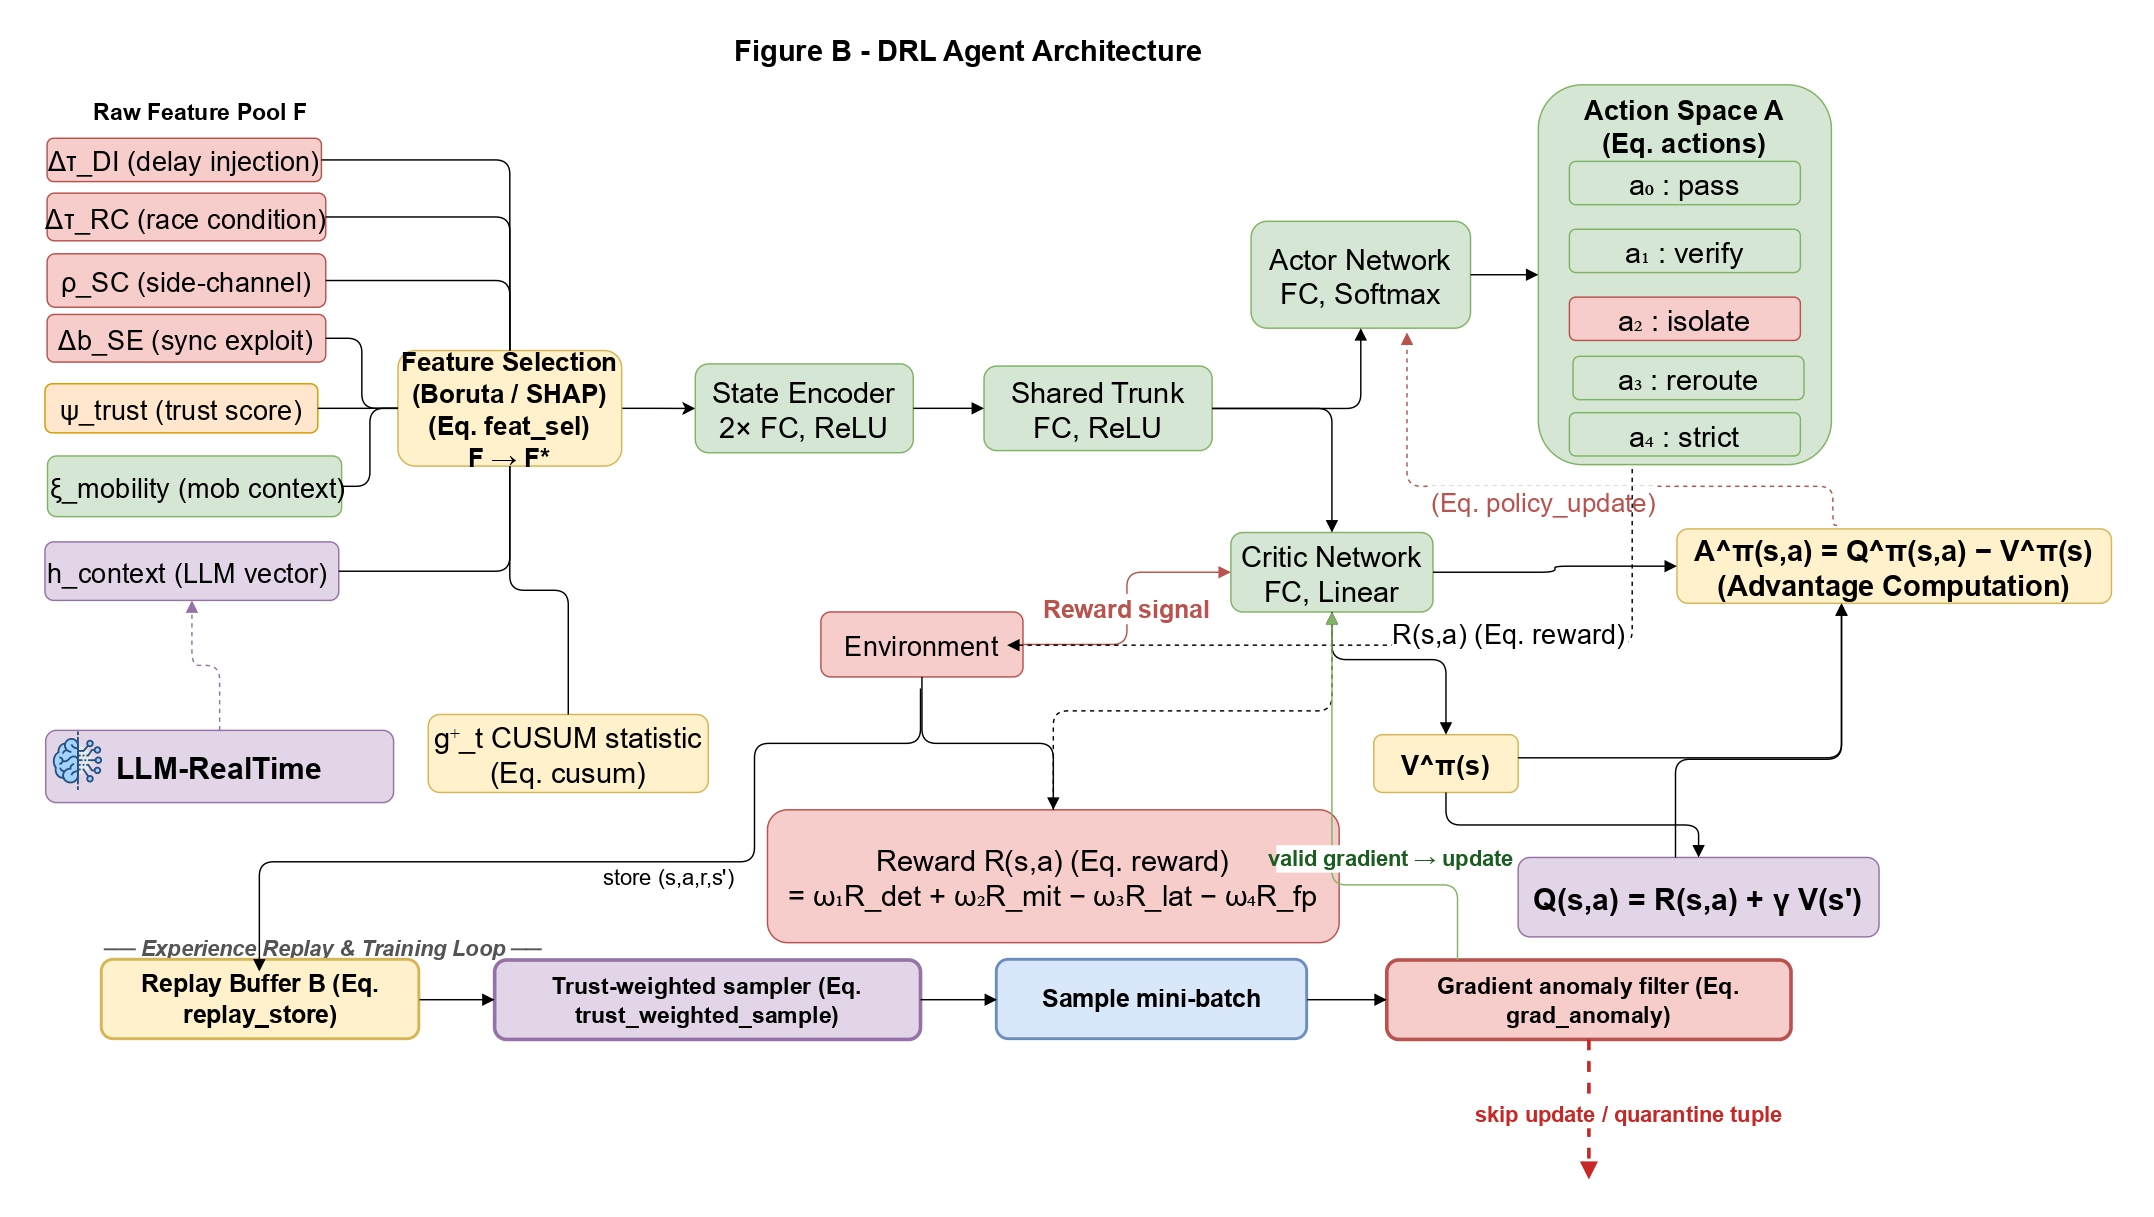
\includegraphics[width=\linewidth]{Progress_Works/DMAP_SDVN/Figure_B_Correct.jpg}
\caption{DRL agent architecture implementing the MDP formulation.}
\label{fig:drl_arch}
\end{figure}
\FloatBarrier
% ====== END FIGURE B ======


As shown in Figure~\ref{fig:drl_arch}, seven raw input
streams pass through Boruta--SHAP feature selection to form
the reduced state $\mathbf{s}_t$, which is encoded and split
into the Actor Network producing action probabilities over the
five actions and the Critic Network estimating $Q(s,a)$, with
the decomposed reward signal from the NS3 environment closing
the training loop.



\begin{comment}
\textbf{DRL Model Placement and Architecture}: The DRL agent is integrated within the SDN controller as a "Security Policy Decision Module," positioned between the event handler and the Flow Mod dispatcher. This placement enables the DRL model to intercept and evaluate control-plane events before flow rule generation, ensuring that conflicting updates are identified and resolved at the controller level where global network visibility exists.

\textbf{DRL Formulation and State Representation}: The DRL agent operates on a compact, measurable state representation that captures essential features of race-condition attacks:

\begin{itemize}
    \item \textbf{Event Timing Features}: Inter-arrival time between conflicting link events ($\Delta t_{\text{event}}$), event burst rate from individual RSUs, temporal clustering of contradictory reports.
    
    \item \textbf{Event Consistency Metrics}: UP $\leftrightarrow$ DOWN flip count within observation windows, fraction of conflicting events from specific RSUs, historical consistency patterns.
    
    \item \textbf{RSU Trust Indicators}: Historical anomaly scores based on timing behavior, blockchain verification outcomes (pass/fail/unknown), cryptographic proof validation results.
    
    \item \textbf{Network Context Information}: Vehicle mobility patterns and speed (to distinguish legitimate rapid topology changes), baseline control-plane round-trip times and jitter measurements.
    
    \item \textbf{Flow-Table Stability Metrics}: Current flow churn rate, number of pending Flow Mods, rule installation success rates.
\end{itemize}

\textbf{DRL Action Space}: The DRL agent selects from several mitigation actions based on the observed state:
\begin{itemize}
    \item \textbf{Micro-Hold Implementation}: Briefly delay conflicting updates (on the order of microseconds) to allow for additional verification.
    
    \item \textbf{Corroboration Request}: Trigger multi-source validation by querying neighboring RSUs or V2V networks for consensus on link state.
    
    \item \textbf{Blockchain Verification}: Initiate immediate verification against immutable timing logs stored on the blockchain.
    
    \item \textbf{Atomic Update Enforcement}: Ensure flow rule updates are applied atomically to prevent partial or conflicting rule installations.
    
    \item \textbf{Rate Limiting and Prioritization}: Temporarily reduce event processing priority for RSUs exhibiting suspicious timing patterns.
\end{itemize}


\begin{comment}
\textbf{DRL Formulation and State Representation.}
The DRL agent operates on a compact, measurable state representation
that captures essential features of timing attacks. Event timing
features include the inter-arrival time between conflicting link
events ($\Delta t_{\mathrm{event}}$), event burst rate from individual
RSUs, and temporal clustering of contradictory reports. Event
consistency metrics track the UP$\leftrightarrow$DOWN flip count
within observation windows, the fraction of conflicting events from
specific RSUs, and historical consistency patterns. RSU trust
indicators comprise historical anomaly scores based on timing
behaviour, blockchain verification outcomes (pass/fail/unknown), and
cryptographic proof validation results. Network context information
captures vehicle mobility patterns and speed to distinguish legitimate
rapid topology changes from adversarial events, alongside baseline
control-plane round-trip times and jitter measurements. Flow-table
stability metrics monitor the current flow churn rate, number of
pending Flow-Mods, and rule installation success rates.

\textbf{DRL Action Space.}
Based on the observed state~\eqref{eq:state}, the DRL agent selects
from five mitigation actions~\eqref{eq:actions}. A micro-hold briefly
delays conflicting updates by a few microseconds to allow additional
verification. A corroboration request triggers multi-source validation
by querying neighbouring RSUs or V2V networks for link-state consensus.
A blockchain verification action initiates immediate cross-checking
against immutable timing logs~\eqref{eq:commitment}. Atomic update
enforcement ensures flow-rule updates are applied atomically to prevent
partial or conflicting rule installations. Rate limiting and
prioritisation temporarily reduces event processing priority for RSUs
exhibiting suspicious timing patterns.


\textbf{Reward Function Design}: The DRL agent's reward function balances security effectiveness with network performance:
\[
R = \alpha \cdot R_{\text{security}} + \beta \cdot R_{\text{performance}} - \gamma \cdot R_{\text{overhead}}
\]
where:
\begin{itemize}
    \item $R_{\text{security}}$ rewards correct detection of race-condition attacks and successful prevention of inconsistent flow table states.
    
    \item $R_{\text{performance}}$ penalizes unnecessary delays in legitimate control-plane operations and maintains network responsiveness.
    
    \item $R_{\text{overhead}}$ accounts for computational and communication costs of mitigation actions.
    
    \item $\alpha$, $\beta$, $\gamma$ are weighting coefficients optimized during training.
\end{itemize}


Algorithm~\ref{alg:rc} handles race condition exploitation
by detecting contradictory event pairs.

\begin{algorithm}[H]
\caption{Race Condition Detection and Mitigation
(\texttt{RC-Defend})}
\label{alg:rc}
\begin{algorithmic}[1]
\small
\Procedure{\texttt{RC-Defend}}
  {$e_{\mathrm{new}},\mathcal{Q},\mathrm{mode},
  \pi_\theta,\mathrm{sk}_{\mathrm{ctrl}}$}
  \State Append $e_{\mathrm{new}}$ to event queue $\mathcal{Q}$
  \For{each $e_{\mathrm{prev}} \in \mathcal{Q}$
    from $\mathrm{src}(e_{\mathrm{new}})$}
    \State $\mathcal{C} \gets
      \mathrm{ConflictCheck}(e_{\mathrm{prev}},e_{\mathrm{new}})$
    \State $\Delta t \gets |t_{e_{\mathrm{new}}}
      - t_{e_{\mathrm{prev}}}|$
    \If{$\mathcal{C}=-1$
        \textbf{and} $\Delta t < \epsilon_{RC}$}
      \State $S_{RC} \gets 1$; break
    \EndIf
  \EndFor
  \If{$S_{RC}=0$}
    \State \textbf{return} \textsc{Benign}
  \EndIf
  \If{$\mathrm{mode} = \mathrm{LW}$}
    \State Hold both conflicting Flow-Mods;
      request re-report from RSU
    \State $\psi_r \gets \psi_r - \Delta_{\mathrm{penalty}}$
    \State \textbf{return}
      $(\textsc{Attack},\mathrm{RC},e_{\mathrm{prev}},
      e_{\mathrm{new}})$
  \EndIf
  \State $\mathbf{s}_t \gets \texttt{BuildState}
    (\Delta\tau^{RC},\boldsymbol{\psi},\boldsymbol{\xi},
    \mathbf{h}^{\mathrm{ctx}})$~\eqref{eq:state}
  \State $a_t \gets \pi_\theta(\mathbf{s}_t)$
  \If{$a_t = a_1^{\mathrm{verify}}$}
    \State Query neighbouring RSUs for consensus
  \ElsIf{$a_t \in
    \{a_2^{\mathrm{isolate}},a_4^{\mathrm{strict}}\}$}
    \State \texttt{SmartContract.EnforceAtomicUpdate}
      $(r,e_{\mathrm{prev}},e_{\mathrm{new}})$
    \State \texttt{PQC-Mitigate}$(r,\mathrm{RC},
      \mathrm{sk}_{\mathrm{ctrl}})$
  \EndIf
  \State $\mathrm{CID} \gets \mathrm{IPFS\_Store}
    (\mathrm{Hash}(e_{\mathrm{prev}}\|e_{\mathrm{new}}\|\Delta t))$
  \State \textbf{return}
    $(\textsc{Attack},\mathrm{RC},a_t,\mathrm{CID})$
\EndProcedure
\end{algorithmic}
\end{algorithm}

As shown in Algorithm~\ref{alg:rc}, each incoming event
is compared against prior events from the same RSU. When
a conflicting pair satisfying $\mathcal{C}=-1$ is found
within the race window $\epsilon_{\mathrm{RC}}$, the
signature fires. In LW mode both conflicting Flow-Mods
are held and a re-report is requested. In Full mode the
DRL agent queries neighbouring RSUs for consensus or
invokes the smart contract to enforce atomic update
semantics.

Algorithm~\ref{alg:sc_def} addresses timing side-channel
attacks by computing correlation-based signatures over a
sliding observation window.

\begin{algorithm}[H]
\caption{Timing Side-Channel Detection and Mitigation
(\texttt{SC-Defend})}
\label{alg:sc_def}
\begin{algorithmic}[1]
\small
\Procedure{\texttt{SC-Defend}}
  {$\mathbf{T}_{1:n},\mathbf{E}_{1:n},\mathrm{mode},
  \pi_\theta,\mathrm{sk}_{\mathrm{ctrl}}$}
  \State $\hat{\rho} \gets
    \mathrm{PearsonCorr}(\mathbf{T}_{1:n},\mathbf{E}_{1:n})$
  \State $\hat{\sigma}_{\mathrm{timing}} \gets
    \mathrm{std}(\mathbf{T}_{1:n})$
  \State $S_{SC} \gets
    \mathbb{1}[\hat{\rho}>\rho_{th}]
    \cdot\mathbb{1}
    [\hat{\sigma}_{\mathrm{timing}}<\theta_{\mathrm{noise}}]$
    \Comment{from~\eqref{eq:sig_sc}}
  \If{$S_{SC}=0$}
    \State \textbf{return} \textsc{Benign}
  \EndIf
  \State Inject noise $\eta \sim
    \mathcal{U}(0,\epsilon_{\mathrm{noise}})$;
    enforce encrypted channels
  \If{$\mathrm{mode} = \mathrm{LW}$}
    \State Log $(\hat{\rho},\hat{\sigma})$; flag RSU
    \State \textbf{return}
      $(\textsc{Attack},\mathrm{SC},\hat{\rho})$
  \EndIf
  \State Switch RSU attestations to ZKP mode
  \State $\mathbf{s}_t \gets \texttt{BuildState}
    (\hat{\rho},\boldsymbol{\psi},\boldsymbol{\xi},
    \mathbf{h}^{\mathrm{ctx}})$~\eqref{eq:state}
  \State $a_t \gets \pi_\theta(\mathbf{s}_t)$
  \If{$a_t \in
    \{a_2^{\mathrm{isolate}},a_4^{\mathrm{strict}}\}$}
    \State \texttt{PQC-Mitigate}$(r,\mathrm{SC},
      \mathrm{sk}_{\mathrm{ctrl}})$
  \EndIf
  \State $\mathrm{CID} \gets \mathrm{IPFS\_Store}
    (\mathrm{Hash}(\hat{\rho}\|\hat{\sigma}\|
    \mathbf{T}_{1:n}))$
  \State \textbf{return}
    $(\textsc{Attack},\mathrm{SC},a_t,\mathrm{CID})$
\EndProcedure
\end{algorithmic}
\end{algorithm}

As shown in Algorithm~\ref{alg:sc_def}, both the Pearson
correlation and the timing standard deviation must
simultaneously exceed their thresholds before the
signature fires, reducing false positives from
congestion-induced correlation. An immediate preventive
action --- injection of calibrated timing noise and
enforcement of encrypted channels --- is applied in both
modes. In Full mode, ZKP attestation mode is additionally
activated so that RSUs never again reveal exact timestamps
during the probationary period.

Algorithm~\ref{alg:se} addresses synchronisation exploits
by monitoring beacon inter-arrival patterns and handover
report timing differentials.

\begin{algorithm}[H]
\caption{Synchronisation Exploit Detection and Mitigation
(\texttt{SE-Defend})}
\label{alg:se}
\begin{algorithmic}[1]
\small
\Procedure{\texttt{SE-Defend}}
  {$\mathbf{b}_{1:n},\mathbf{R}_t,\mathrm{mode},
  \pi_\theta,\mathrm{sk}_{\mathrm{ctrl}}$}
  \State $\mathrm{gap} \gets
    \exists\,k:\;b_k > 2/f_{\mathrm{beacon}}$
  \State $\mathrm{var} \gets
    \frac{1}{n}\sum_{i=1}^{n}(b_i-\bar{b})^2$
  \State $S_{SE}^{\mathrm{beacon}} \gets
    \mathbb{1}[\mathrm{gap}]
    \cdot\mathbb{1}[\mathrm{var}>\theta_{SE}^2]$
  \State $\Delta\tau_{\mathrm{HO}} \gets
    |T_{\mathrm{report}}^{r_A} - T_{\mathrm{report}}^{r_B}|$
  \State $S_{SE} \gets S_{SE}^{\mathrm{beacon}}
    \vee \mathbb{1}[\Delta\tau_{\mathrm{HO}} >
    \theta_{\mathrm{HO}}(\hat{v}_k)]$
  \If{$S_{SE}=0$}
    \State \textbf{return} \textsc{Benign}
  \EndIf
  \If{$\mathrm{mode} = \mathrm{LW}$}
    \State Require 3 consecutive valid beacons
      before handover commit
    \State $\psi_r \gets \psi_r - \Delta_{\mathrm{penalty}}$
    \State \textbf{return}
      $(\textsc{Attack},\mathrm{SE},\mathrm{var},
      \Delta\tau_{\mathrm{HO}})$
  \EndIf
  \State Validate vehicle trajectory plausibility
  \State Request corroboration from $\geq t$ RSUs
  \State $\mathbf{s}_t \gets \texttt{BuildState}
    (\Delta b,\boldsymbol{\psi},\boldsymbol{\xi},
    \mathbf{h}^{\mathrm{ctx}})$~\eqref{eq:state}
  \State $a_t \gets \pi_\theta(\mathbf{s}_t)$
  \If{$a_t \in
    \{a_2^{\mathrm{isolate}},a_3^{\mathrm{reroute}}\}$}
    \State \texttt{PQC-Mitigate}$(r,\mathrm{SE},
      \mathrm{sk}_{\mathrm{ctrl}})$
  \EndIf
  \State $\mathrm{CID} \gets \mathrm{IPFS\_Store}
    (\mathrm{Hash}(\mathrm{var}\|\Delta\tau_{\mathrm{HO}}))$
  \State \textbf{return}
    $(\textsc{Attack},\mathrm{SE},a_t,\mathrm{CID})$
\EndProcedure
\end{algorithmic}
\end{algorithm}

As shown in Algorithm~\ref{alg:se}, the beacon check and
handover timing differential check are evaluated
independently and combined with logical OR, so either
condition alone triggers detection. In LW mode, a
hysteresis guard requiring three consecutive valid beacons
prevents oscillation attacks from causing repeated
unnecessary handovers. In Full mode, the DRL agent
validates the vehicle trajectory and requests
threshold-signed corroboration from neighbouring RSUs
before committing a handover decision.

\paragraph{Integration with Blockchain and LLM Components}
The DRL-based race-condition mitigation integrates with other defense framework components:

\begin{itemize}
    \item \textbf{Blockchain Integration}: The DRL agent queries the blockchain for immutable timing records to validate event sequences and detect timing inconsistencies that might indicate race-condition attacks.
    
    \item \textbf{LLM Contextual Analysis}: When race conditions are detected, LLMs analyze the sequence of events to generate human-readable explanations, distinguishing between legitimate rapid topology changes and malicious race-condition exploitation.
    
    \item \textbf{Trust Management Updates}: Successful detection of race-condition attacks reduces the trust score of compromised RSUs, while false positives incrementally restore trust based on verified legitimate behavior.
\end{itemize}
\end{comment}


Algorithm~\ref{alg:drl} presents the online DRL detection
loop implementing the actor-critic training procedure.

\begin{algorithm}[H]
\caption{DRL-Based Adaptive Detection (\texttt{DRL-Detect})}
\label{alg:drl}
\begin{algorithmic}[1]
\small
\Procedure{\texttt{DRL-Detect}}{$\mathbf{s}_0,\pi_\theta,T$}
  \State Initialise replay buffer $\mathcal{B}\gets\emptyset$
  \For{$t=0,1,\ldots,T$}
    \State $a_t\gets\pi_\theta(\mathbf{s}_t)$
      \Comment{actor selects action~\eqref{eq:actions}}
    \State Execute $a_t$; observe $\mathbf{s}_{t+1}$,
      $r_t\gets R(\mathbf{s}_t,a_t)$
    \State $\mathcal{B}\gets
      \mathcal{B}\cup\{(\mathbf{s}_t,a_t,r_t,
      \mathbf{s}_{t+1})\}$
    \If{$|\mathcal{B}|\geq B_{\min}$}
      \State Sample mini-batch $\mathcal{B}'\sim\mathcal{B}$
      \State $\hat{Q}\gets r+\gamma\max_{a'}
        Q(\mathbf{s}_{t+1},a')$
      \State Update critic: $\nabla_\phi\gets
        \mathbb{E}_{\mathcal{B}'}
        [(Q_\phi(\mathbf{s},a)-\hat{Q})^2]$
      \State Update actor: $\nabla_\theta\gets
        \mathbb{E}_{\mathcal{B}'}
        [\nabla_\theta\log\pi_\theta\cdot A^\pi]$
      \State Update $\phi,\theta$ via gradient descent
    \EndIf
    \State $\mathbf{s}_t\gets\mathbf{s}_{t+1}$
  \EndFor
\EndProcedure
\end{algorithmic}
\end{algorithm}

As shown in Algorithm~\ref{alg:drl}, at each epoch the
actor network selects an action from the five-element
action space~\eqref{eq:actions}. The environment returns
the next state and the composite reward
$R(\mathbf{s}_t, a_t)$~\eqref{eq:reward}, stored in the
replay buffer $\mathcal{B}$. Once the buffer exceeds
$B_{\min}$, a mini-batch is sampled and both the critic
(minimising Bellman error~\eqref{eq:bellman}) and the
actor (maximising advantage-weighted log-probability via
\eqref{eq:policy}) are updated via gradient descent,
stabilising training under the non-stationary timing
distributions induced by vehicular mobility.

\begin{comment}
...
\end{comment}

\subsubsection{Blockchain Smart-Contract and IPFS Integration}
\label{sec:blockchain}

The blockchain layer serves two distinct roles: a \emph{detection role}
— aggregating tamper-evident timing proof commitments across RSUs to
enable consensus-based anomaly confirmation — and a \emph{mitigation
role} — enforcing trust revocation and RSU isolation via immutable smart
contract execution. The two roles are implemented as separate chaincode
functions on Hyperledger Fabric.

\textbf{Timing Proof Commitment.}
Each RSU $r$ generates a commitment for every processed control
message $m_{ij}$, as defined in Equation~\eqref{eq:commitment}.
\begin{equation}
C_{ij} = \mathrm{Hash}\!\left(
  \mathrm{msg\_id} \;\|\;
  T_{\mathrm{obs}}^{ij} \;\|\;
  \Delta T^{ij} \;\|\;
  \sigma_{\mathrm{ML\text{-}DSA}}(m_{ij})
\right),
\label{eq:commitment}
\end{equation}
As shown in Equation~\eqref{eq:commitment}, $\Delta T^{ij} =
T_{\mathrm{obs}}^{ij} - T_{\mathrm{exp}}^{ij}$ is the observed
timing deviation and $\sigma_{\mathrm{ML\text{-}DSA}}(m_{ij})$
is the PQC signature of the message defined in~\eqref{eq:sign}.
The commitment is stored in IPFS and anchored to the blockchain
as defined in Equation~\eqref{eq:cid} and
Equation~\eqref{eq:block} respectively.
\begin{equation}
\mathrm{CID}_t = \mathrm{IPFS\_Hash}(C_{ij} \;\|\; \mathrm{epoch}_t),
\label{eq:cid}
\end{equation}
As shown in Equation~\eqref{eq:cid}, the content identifier
$\mathrm{CID}_t$ is derived from the commitment $C_{ij}$ and
the current epoch, enabling content-addressable retrieval.
\begin{equation}
B_t = \mathrm{Block}\!\left(
  \mathrm{CID}_t,\;
  \mathrm{Hash}(B_{t-1}),\;
  \sigma_{\mathrm{ML\text{-}DSA}}^{\mathrm{ctrl}}
\right).
\label{eq:block}
\end{equation}
As shown in Equation~\eqref{eq:block}, the blockchain block
$B_t$ chains the CID with the previous block hash and a
controller ML-DSA signature, providing tamper-evident immutable
anchoring. IPFS provides content-addressable decentralised
storage, enabling real-time evidence anchoring without requiring
all Fabric peers to be synchronised before the evidence is
queryable.

\textbf{Consensus Validity Condition.}
A timing proof is accepted by the smart contract only when a
sufficient quorum of RSUs independently confirm it, as defined
in Equation~\eqref{eq:consensus}.
\begin{equation}
\mathrm{Valid}(C_{ij}) =
  \mathbb{1}\!\left[
    \sum_{r\in\mathcal{V}_r}
    \mathbb{1}[\mathrm{verify}_r(C_{ij})=1]
    \geq
    \left\lceil f_{\mathrm{cons}}\cdot|\mathcal{V}_r|\right\rceil
  \right],
\label{eq:consensus}
\end{equation}
As shown in Equation~\eqref{eq:consensus}, $f_{\mathrm{cons}}$
is the consensus fraction, set to $2/3$ for Byzantine fault
tolerance. A proof failing this condition triggers escalation
to the DRL agent.

\textbf{Reputation-Weighted Consensus.}
Extending the digit-coin reputation mechanism
of~\cite{alkhamisi2024bcs} to timing-proof validation,
each RSU vote in the consensus~\eqref{eq:consensus}
is weighted by its current trust score, as defined in
Equation~\eqref{eq:weighted_cons}.
\begin{equation}
W_{\mathrm{cons}}(C_{ij}) =
  \frac{\sum_{r\in\mathcal{V}_r}
    \psi_r(t)\cdot\mathbb{1}[\mathrm{verify}_r(C_{ij})=1]}
  {\sum_{r\in\mathcal{V}_r}\psi_r(t)},
\label{eq:weighted_cons}
\end{equation}
As shown in Equation~\eqref{eq:weighted_cons}, acceptance
requires $W_{\mathrm{cons}}(C_{ij}) \geq f_{\mathrm{cons}}$. This replaces the unweighted
majority in~\eqref{eq:consensus} in Full mode,
ensuring that votes from high-trust RSUs carry
more weight than recently flagged ones, improving
consensus accuracy under partial compromise without
increasing communication overhead.

\textbf{Trust Score Update (Mitigation Role).}
RSU trust scores are maintained by the smart contract and updated
after each epoch, as defined in Equation~\eqref{eq:trust_update}.
\begin{equation}
\psi_r(t{+}1) =
  \lambda_{\mathrm{tr}}\,\psi_r(t) +
  (1-\lambda_{\mathrm{tr}})\,
  \mathbb{1}[\text{no attack flagged from RSU }r],
\label{eq:trust_update}
\end{equation}
As shown in Equation~\eqref{eq:trust_update},
$\lambda_{\mathrm{tr}}\in(0,1)$ is the exponential forgetting
factor that controls how quickly past behaviour is discounted. 

\paragraph{RSU Trust Bootstrapping}
\label{sec:trust_bootstrap}

A newly registering RSU must not immediately receive full consensus
weight, as this would allow an attacker who introduces a new RSU
identity to influence reputation-weighted consensus from the first
epoch. The initial trust score at registration is given in
Equation~\eqref{eq:trust_init}.
%
\begin{equation}
  \psi_r(0) \;=\; \psi_{\mathrm{init}}, \qquad
  \psi_{\mathrm{init}} = 0.10 \;\ll\; \psi_{\mathrm{promote}} = 0.60,
  \label{eq:trust_init}
\end{equation}
%
As given in Equation~\eqref{eq:trust_init}, the initial score
$\psi_{\mathrm{init}}=0.10$ is far below the promotion threshold
$\psi_{\mathrm{promote}}=0.60$, so the new RSU participates in
consensus with negligible weight. Promotion to full endorsing peer
requires both a minimum count of successfully verified timing proof
submissions and a trust score above the promotion threshold. The
promotion condition is given in Equation~\eqref{eq:trust_promote}.
%
\begin{equation}
  \mathrm{promote}(r) \;\Leftrightarrow\;
    n_{\mathrm{verified}}(r) \;\geq\; k_{\min}
    \;\;\text{and}\;\;
    \psi_r \;\geq\; \psi_{\mathrm{promote}},
  \label{eq:trust_promote}
\end{equation}
%
As given in Equation~\eqref{eq:trust_promote},
$n_{\mathrm{verified}}(r)$ is the count of timing proofs from RSU
$r$ that have been verified by the smart contract without dispute,
and $k_{\min}$ is the minimum number of clean submissions required
before endorsing peer rights are granted. The smart contract
enforces this transition; no controller can bypass it.

\paragraph{Quarantine Recovery Protocol}
\label{sec:quarantine_recovery}

Algorithm~\ref{alg:pqc} sets $\psi_{r^*}=0$ and broadcasts a
quarantine command but does not define what happens afterwards.
Without a recovery protocol, sequential quarantine events
permanently reduce $|\mathcal{V}_r^{\mathrm{active}}|$ below the
quorum threshold $t$, causing liveness failure. A quarantined RSU
transitions through four states: \textsc{Active},
\textsc{Quarantine}, \textsc{Probation}, and \textsc{Candidate}.
The state transition function is given in
Equation~\eqref{eq:quarantine_fsm}.
%
\begin{equation}
  \mathrm{state}_r(t{+}1) \;=\;
  \begin{cases}
    \textsc{Quarantine} &
      \text{if } \psi_r(t) < \psi_{\mathrm{low}} \\[2pt]
    \textsc{Probation}  &
      \text{if } \mathrm{state}_r(t)=\textsc{Quarantine}
      \;\wedge\; \psi_r(t) \geq \psi_{\mathrm{low}} \\[2pt]
    \textsc{Candidate}  &
      \text{if } \mathrm{state}_r(t)=\textsc{Probation}
      \;\wedge\; n_{\mathrm{clean}}(r) \geq N_{\mathrm{recover}} \\[2pt]
    \textsc{Active}     &
      \text{if } \mathrm{state}_r(t)=\textsc{Candidate}
      \;\wedge\; \psi_r(t) \geq \psi_{\mathrm{restore}} \\[2pt]
    \mathrm{state}_r(t) & \text{otherwise,}
  \end{cases}
  \label{eq:quarantine_fsm}
\end{equation}
%
As given in Equation~\eqref{eq:quarantine_fsm}, during
\textsc{Probation} the RSU operates as a Fabric lightweight client
only --- it submits signed timing proofs but carries no endorsement
weight in the quorum, so its trustworthiness is evaluated without
allowing it to influence consensus. Promotion to \textsc{Candidate}
requires $N_{\mathrm{recover}}$ consecutive clean epochs (no
flagged events); promotion to \textsc{Active} additionally requires
$\psi_r \geq \psi_{\mathrm{restore}}$. After each state transition
the smart contract recomputes the active quorum $t(t)$ using
Equation~\eqref{eq:dynamic_quorum}.


When $\psi_r(t)<\psi_{\mathrm{low}}$, the smart contract
automatically executes an isolation command: a PQC-signed
\texttt{QUARANTINE}$(r)$ transaction is broadcast to all RSUs,
rerouting control traffic away from $r$ until $\psi_r$ recovers
above $\psi_{\mathrm{restore}}$ through a probationary period.
This constitutes the \emph{mitigation role} of the blockchain layer,
executing enforcement without requiring controller intervention and
thus providing tamper-proof, auditable mitigation records.


The threat model in Section~\ref{sec:threat_model} states that
the attacker can compromise vehicular nodes. Yet the existing
design maintains trust scores only for RSUs ($\psi_r$), leaving
vehicles --- which trigger handover reports, send beacons, and
initiate uplink control messages --- entirely unaccountable. To
address this asymmetry, each vehicle $v_k \in \mathcal{V}_v(t)$
is assigned a trust score $\psi_{v_k}(t)$ maintained by the
smart contract using the same exponential moving average as RSU
trust. The vehicle trust update rule is given in
Equation~\eqref{eq:vehicle_trust_update}.
%
\begin{equation}
  \psi_{v_k}(t{+}1) \;=\;
    \lambda_v\,\psi_{v_k}(t)
    \;+\;
    (1-\lambda_v)\,
    \mathbb{1}\bigl[
      \text{no misbehaviour from } v_k \text{ at } t
    \bigr],
  \label{eq:vehicle_trust_update}
\end{equation}
%
As given in Equation~\eqref{eq:vehicle_trust_update},
$\lambda_v \in (0,1)$ is the vehicle trust forgetting factor.
Vehicle misbehaviour is detected through V2V cross-verification:
each vehicle's self-reported mobility state is compared against
observations by physically neighbouring vehicles. The
V2V cross-verification discrepancy is given in
Equation~\eqref{eq:v2v_cross}.
%
\begin{equation}
  \Delta_{\mathrm{V2V}}^{v_k} \;=\;
    \left|
      \xi_k^{\mathrm{self}}(t)
      \;-\;
      \underset{v_{k^{\prime}} \in \mathcal{N}(v_k)}{\mathrm{median}}\;
      \xi_{k^{\prime}}^{\mathrm{obs}}(t)
    \right|,
  \label{eq:v2v_cross}
\end{equation}
%
As given in Equation~\eqref{eq:v2v_cross},
$\xi_k^{\mathrm{self}}(t)$ is the mobility state self-reported
by $v_k$ and $\xi_{k^{\prime}}^{\mathrm{obs}}(t)$ is the state
of $v_k$ as independently observed by neighbour $v_{k^{\prime}}$.
A large $\Delta_{\mathrm{V2V}}^{v_k}$ indicates falsified
mobility state, which an attacker could use to engineer
synchronisation exploits or race conditions. Vehicle misbehaviour
reports are submitted by RSUs to the smart contract, which
decrements $\psi_{v_k}$ accordingly. The vehicle trust score
$\psi_{v_k}(t)$ is added to the per-event LLM input feature
vector $x_l^r$ in Equation~\eqref{eq:llm_input}, and is included
in the DRL state vector $\mathbf{s}_t$ of
Equation~\eqref{eq:state} as part of the trust subvector
$\boldsymbol{\psi}_t^{\mathrm{trust}}$. Vehicle trust is
bootstrapped at $\psi_{v_k}(0) = \psi_{\mathrm{init}}$
(Equation~\eqref{eq:trust_init}) and promoted following
Equation~\eqref{eq:trust_promote}, with
$n_{\mathrm{verified}}(v_k)$ counting successful V2V-confirmed
mobility reports.


\paragraph{Controller Trust Scoring}
\label{sec:ctrl_trust}

Controller behaviour is monitored by RSU consensus; no controller
can report on or modify its own trust score. Each RSU $r$
independently checks whether the flow rules received from
controller $c_k$ are consistent with its locally observed
network state and with the majority view of neighbouring RSUs.
The per-RSU controller misbehaviour indicator is given in
Equation~\eqref{eq:ctrl_misbehave}.
%
\begin{equation}
  M_{c_k}^{r}(t) \;=\; \mathbb{1}\!\left[
    \frac{
      \bigl|\{\text{FlowRules}_{c_k}^{r}(t)\;
             \text{inconsistent with}\;
             \mathrm{ConsensusView}_{r}(t)\}\bigr|
    }{
      \bigl|\text{FlowRules}_{c_k}^{r}(t)\bigr|
    } \;>\; \eta_c
  \right],
  \label{eq:ctrl_misbehave}
\end{equation}
%
As given in Equation~\eqref{eq:ctrl_misbehave}, $\eta_c$ is the
maximum tolerable fraction of inconsistent flow rules before
misbehaviour is declared; $\mathrm{ConsensusView}_{r}(t)$ is the
RSU's local estimate of expected rules given its observed network
topology. Each RSU submits $M_{c_k}^{r}(t)$ as a signed report
to the Hyperledger Fabric smart contract, which aggregates across
all RSUs and updates the controller trust score. The controller
trust update rule is given in
Equation~\eqref{eq:ctrl_trust_update}.
%
\begin{equation}
  \psi_{c_k}(t{+}1) \;=\;
    \lambda_{\mathrm{ctrl}}\,\psi_{c_k}(t)
    \;+\;
    (1-\lambda_{\mathrm{ctrl}})\,
    \mathbb{1}\!\left[
      \frac{1}{|\mathcal{V}_r|}
      \sum_{r \in \mathcal{V}_r} M_{c_k}^{r}(t)
      \;<\; \eta_c
    \right],
  \label{eq:ctrl_trust_update}
\end{equation}
%
As given in Equation~\eqref{eq:ctrl_trust_update},
$\lambda_{\mathrm{ctrl}} \in (0,1)$ is the forgetting factor
that discounts past behaviour. The smart contract---not any
controller---executes this update. When $\psi_{c_k}(t) 
\psi_{\mathrm{low}}^{\mathrm{ctrl}}$, the smart contract
initiates a trust-verified failover to the highest-trust
available peer. The failover target selection rule is given in
Equation~\eqref{eq:ctrl_failover}.
%
\begin{equation}
  c^{*} \;=\;
    \arg\max_{\substack{c_k \in \mathcal{C} \\ \psi_{c_k}(t)\;>\;\psi_{\mathrm{low}}^{\mathrm{ctrl}}}}
    \psi_{c_k}(t),
  \label{eq:ctrl_failover}
\end{equation}
%
As given in Equation~\eqref{eq:ctrl_failover}, the failover
target is always the peer with the highest current trust score
rather than a predetermined backup, so an attacker cannot
predict and pre-compromise the failover destination. The failover
command is co-authorised by a quorum of RSU signatures, ensuring
that no compromised controller can redirect traffic to a
co-conspirator.

Algorithm~\ref{alg:sc} defines the Hyperledger Fabric
smart contract chaincode for timing-proof submission,
consensus validation, and trust management.

\begin{algorithm}[H]
\caption{Smart Contract Trust Management (\texttt{SC-TrustMgr})}
\label{alg:sc}
\begin{algorithmic}[1]
\small
\Procedure{\texttt{SubmitTimingProof}}{$r,C_{ij},\sigma_r$}
  \State $b\gets\mathrm{ML\text{-}DSA.Verify}
    (\mathrm{pk}_r,C_{ij},\sigma_r)$
  \If{$b=0$} \textbf{return} \textsc{Reject} \EndIf
  \State \texttt{ledger}[$r$].\texttt{append}$(C_{ij})$
  \State $n_c\gets|\{r'\in\mathcal{V}_r:
    \mathrm{verify}_{r'}(C_{ij})=1\}|$
  \If{$n_c\geq\lceil f_{\mathrm{cons}}
      \cdot|\mathcal{V}_r|\rceil$}
    \State \texttt{ledger.anchor}$(\mathrm{CID}_{C_{ij}})$
    \State \textbf{return} \textsc{Accept}
  \Else\; \textbf{return} \textsc{Pending}
  \EndIf
\EndProcedure
\vspace{0.4em}
\Procedure{\texttt{UpdateTrust}}{$r,\mathrm{flagged}$}
  \If{\textbf{not} $\mathrm{flagged}$}
    \State $\psi_r\gets
      \lambda_{\mathrm{tr}}\psi_r+(1{-}\lambda_{\mathrm{tr}})$
  \Else
    \State $\psi_r\gets
      \max(0,\psi_r-\Delta_{\mathrm{penalty}})$
  \EndIf
  \If{$\psi_r<\psi_{\mathrm{low}}$}
    \State \texttt{PQC-Mitigate}$(r,\mathrm{flagged},
      \mathrm{sk}_{\mathrm{ctrl}})$
  \EndIf
\EndProcedure
\end{algorithmic}
\end{algorithm}

As shown in Algorithm~\ref{alg:sc}, the
\texttt{SubmitTimingProof} procedure first verifies the
ML-DSA signature and rejects unsigned proofs immediately.
It then counts independent RSU verifications and accepts
the proof only when the quorum
$\lceil f_{\mathrm{cons}} \cdot |\mathcal{V}_r| \rceil$
is reached. The \texttt{UpdateTrust} procedure applies an
exponential moving average for benign RSUs and a penalty
decrement for flagged ones, automatically triggering
\texttt{PQC-Mitigate} when the trust score falls below
$\psi_{\mathrm{low}}$.


% ====== FIGURE C — CORRECTED ======
The end-to-end interaction sequence of the blockchain layer is
depicted in Figure~\ref{fig:blockchain_seq}. The five vertical
lifelines represent the RSU, IPFS, Smart Contract, Blockchain
Ledger, and SDN Controller.

Step~\textcircled{1}: RSU $r$ computes the timing-proof
commitment $C_{ij}$~\eqref{eq:commitment} and stores it in
IPFS. Step~\textcircled{2}: IPFS returns a content identifier
$\mathrm{CID}_t$~\eqref{eq:cid}, making the evidence
immediately queryable without waiting for blockchain consensus.
Step~\textcircled{3}: RSU $r$ calls
\texttt{SC-TrustMgr.SubmitTimingProof}
(Algorithm~\ref{alg:sc}) on the smart contract.
Steps~\textcircled{4a}--\textcircled{4c}: the smart contract
performs ML-DSA signature verification~\eqref{eq:verify},
checks the $t$-of-$n$ threshold
quorum~\eqref{eq:thresh_verify}, and evaluates the
reputation-weighted consensus condition
$W_{\mathrm{cons}}(C_{ij}) \geq
f_{\mathrm{cons}}$~\eqref{eq:weighted_cons}.
Step~\textcircled{4d}: if the proof is valid, the CID is
anchored to the Blockchain Ledger~\eqref{eq:block}.
Step~\textcircled{5}: the validation result
$\mathrm{Valid}(C_{ij})$~\eqref{eq:consensus} is returned to
the SDN Controller. Step~\textcircled{6} (red dashed path):
if consensus fails, a \textsc{REJECT} is sent back to the RSU,
serving as detection evidence of a compromised RSU.
Step~\textcircled{7}: the controller invokes
\texttt{UpdateTrust}$(r, \mathrm{flagged})$~\eqref{eq:trust_update}.
Step~\textcircled{8}: if $\psi_r < \psi_{\mathrm{low}}$, the
smart contract autonomously triggers \textsc{PQC-Mitigate}
(Algorithm~\ref{alg:pqc}), enforcing RSU isolation without
requiring manual controller intervention.

\begin{figure}[htb]
\centering
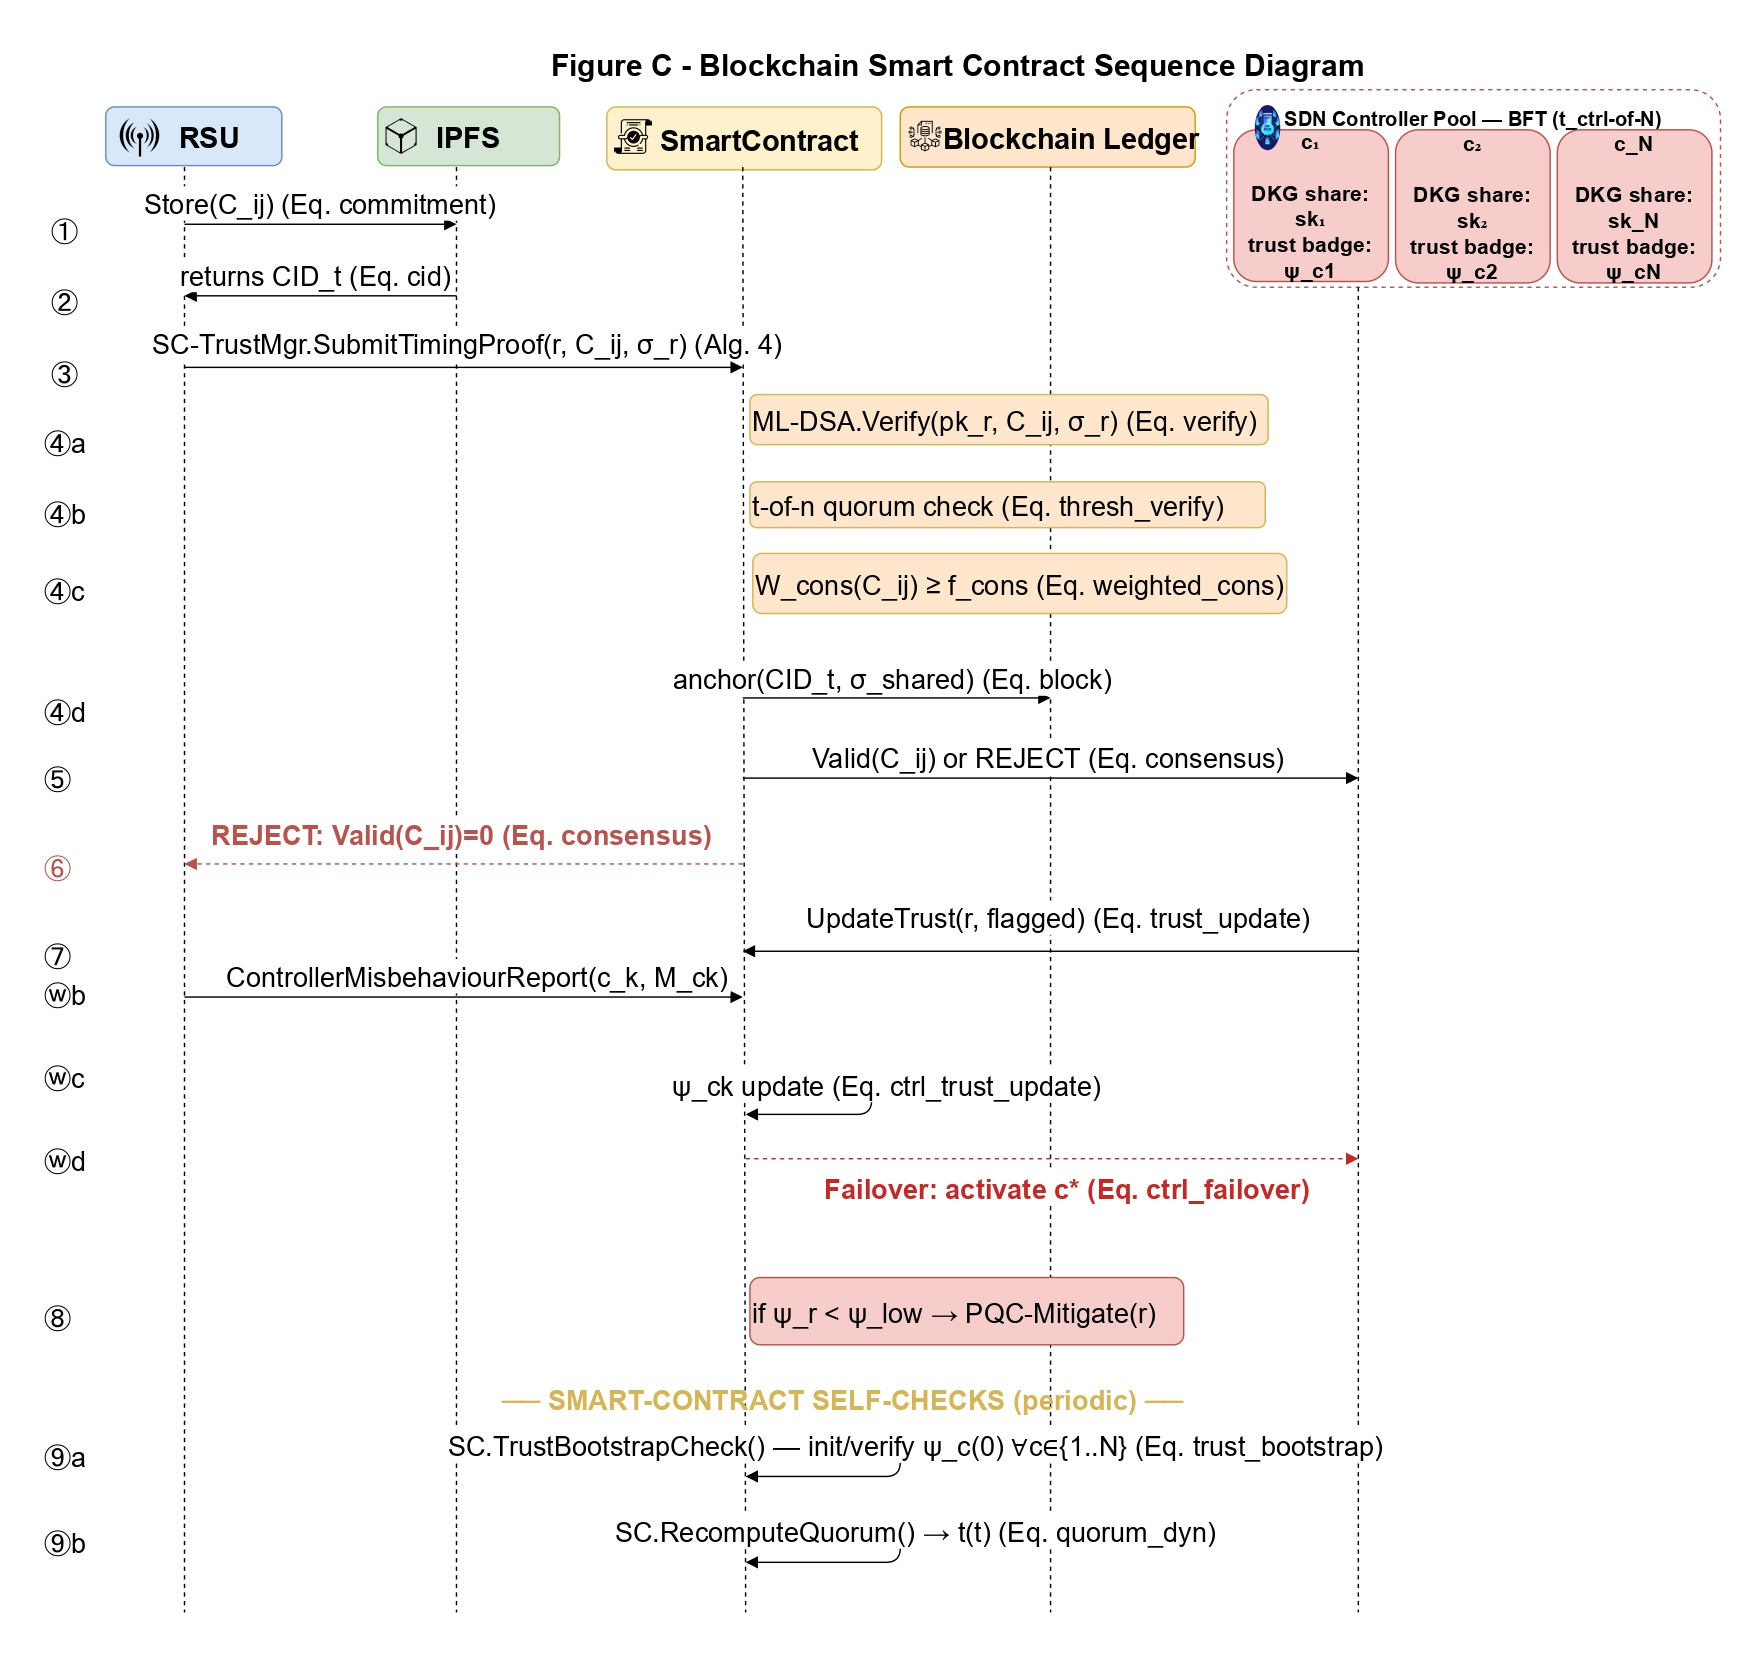
\includegraphics[width=\linewidth]{Progress_Works/DMAP_SDVN/Figure_C_Correct_2.jpg}
\caption{Smart contract interaction sequence for timing-proof submission, consensus validation, and trust-based mitigation.}
\label{fig:blockchain_seq}
\end{figure}
\FloatBarrier
% ====== END FIGURE C ======


As shown in Figure~\ref{fig:blockchain_seq}, the RSU first
anchors the timing-proof commitment to IPFS and receives a CID
before calling the smart contract, which performs ML-DSA
verification and reputation-weighted consensus validation
before anchoring to the blockchain ledger. When consensus
fails, the REJECT path triggers trust score decrement and
autonomous RSU isolation via \textsc{PQC-Mitigate} without
requiring manual controller intervention.


\begin{comment}
...
\end{comment}


\subsubsection{Post-Quantum Cryptographic Layer}
\label{sec:pqc}

Three complementary cryptographic primitives are selected from the
mandated set, each justified by the specific attack geometry of SDVN
timing attacks.

\textbf{(i) CRYSTALS-Dilithium / ML-DSA (FIPS 204) — Mandatory PQC.}
ML-DSA is selected as the primary signing scheme for all control-plane
messages (Flow-Mod, beacons, RSU event reports) because its 0.65\,ms
signing latency on standard embedded hardware is compatible with SDVN
timing constraints, and its security rests on the hardness of the
Module Short Integer Solution (MSIS) and Module Learning With Errors
(MLWE) problems, providing 128-bit post-quantum security at Level~2.
Key generation, signing, and verification are formalised in
Equations~\eqref{eq:keygen}--\eqref{eq:verify}.
\begin{align}
(\mathrm{pk},\mathrm{sk})
  &\leftarrow \mathrm{ML\text{-}DSA.KeyGen}(\lambda),
  \label{eq:keygen} \\
\sigma_{m}
  &= \mathrm{ML\text{-}DSA.Sign}\!\left(
      \mathrm{sk},\;
      m_{ij} \;\|\; T_{\mathrm{obs}}^{ij} \;\|\; \mathrm{nonce}
    \right),
  \label{eq:sign} \\
\mathrm{valid}
  &= \mathrm{ML\text{-}DSA.Verify}\!\left(
      \mathrm{pk},\;
      m_{ij} \;\|\; T_{\mathrm{obs}}^{ij} \;\|\; \mathrm{nonce},\;
      \sigma_m
    \right).
  \label{eq:verify}
\end{align}
As shown in Equations~\eqref{eq:keygen}--\eqref{eq:verify},
key generation produces a public-private key pair, signing
binds the message, observed timestamp, and nonce to produce
$\sigma_m$, and verification confirms the signature against
the same payload. Any RSU receiving a Flow-Mod or beacon
with an invalid $\sigma_m$ immediately rejects the message and logs the
rejection to IPFS~\eqref{eq:cid}. Including $T_{\mathrm{obs}}^{ij}$
in the signed payload binds each signature to a specific timing claim,
making delay-and-replay attacks cryptographically detectable.

\paragraph{Distributed Key Generation for Controller Signing}
\label{sec:dkg}

No single controller holds the full control-plane signing key.
A Distributed Key Generation (DKG) protocol produces one shared
public key and per-controller secret shares so that
$t_{\mathrm{ctrl}}$-of-$N$ controllers must cooperate to produce
any valid signature. The DKG setup is given in
Equation~\eqref{eq:dkg_setup}.
%
\begin{equation}
  \bigl(
    \mathrm{pk}_{\mathrm{shared}},\;
    \{\mathrm{sk}_i\}_{i=1}^{N}
  \bigr)
  \;\leftarrow\;
  \mathrm{DKG.Setup}(\lambda,\, N,\, t_{\mathrm{ctrl}}),
  \label{eq:dkg_setup}
\end{equation}
%
As given in Equation~\eqref{eq:dkg_setup}, $\lambda$ is the
security parameter, $N$ is the total controller count, and
$t_{\mathrm{ctrl}} = \lceil N/2 \rceil + 1$ is the signing
threshold. No individual $\mathrm{sk}_i$ can reconstruct the
full key; a Byzantine minority of controllers therefore cannot
forge signatures unilaterally.

Threshold signature aggregation requiring at least
$t_{\mathrm{ctrl}}$ cooperating controllers is given in
Equation~\eqref{eq:thresh_ctrl_sign}.
%
\begin{equation}
  \sigma_{\mathrm{shared}} \;=\;
    \mathrm{ThreshSign}\!\bigl(
      \{\mathrm{sk}_i\}_{i \in \mathcal{S}},\; m
    \bigr),
    \quad |\mathcal{S}| \geq t_{\mathrm{ctrl}},
  \label{eq:thresh_ctrl_sign}
\end{equation}
%
As given in Equation~\eqref{eq:thresh_ctrl_sign}, any qualifying
subset $\mathcal{S}$ of at least $t_{\mathrm{ctrl}}$ controllers
jointly produces $\sigma_{\mathrm{shared}}$, which is verified
by RSUs using $\mathrm{pk}_{\mathrm{shared}}$ with the unchanged
$\mathrm{ML\text{-}DSA.Verify}$ procedure of
Equation~\eqref{eq:verify}. All Flow-Mod messages, quarantine
commands, and blockchain block anchors use
$\sigma_{\mathrm{shared}}$ in place of the former single-controller
signature, so no single compromised controller can forge or
suppress any of these critical artefacts.


\paragraph{Cross-RSU Timestamp Verification}
\label{sec:timestamp_verify}

The ML-DSA signature in Equation~\eqref{eq:sign} proves that the
controller or RSU holding the signing key \emph{claimed}
$T_{\mathrm{obs}}^{ij}$, but cannot prove the claim is truthful.
A compromised insider RSU can sign any timestamp it chooses,
fabricating timing evidence while the signature still verifies
correctly. To close this gap, each RSU cross-checks its
self-reported observed timestamp against independent observations
from its physical neighbours in the same coverage zone.

The neighbourhood consensus timestamp, computed as a
Byzantine-robust median over neighbour observations, is given in
Equation~\eqref{eq:cross_ts_median}.
%
\begin{equation}
  \bar{T}_{\mathrm{obs}}^{ij} \;=\;
    \underset{r^{\prime} \in \mathcal{N}(r)}{\mathrm{median}}\;
    T_{\mathrm{obs},r^{\prime}}^{ij},
  \label{eq:cross_ts_median}
\end{equation}
%
As given in Equation~\eqref{eq:cross_ts_median},
$\mathcal{N}(r)$ is the set of RSUs within wireless communication
range of RSU $r$ that independently observed or proxied message
$m_{ij}$. The median is used rather than the mean to resist
manipulation by a minority of Byzantine neighbours.

The scalar discrepancy between RSU $r$'s self-reported timestamp
and the neighbourhood consensus is given in
Equation~\eqref{eq:cross_ts_disc}.
%
\begin{equation}
  \Delta_{\mathrm{verify}}^{r} \;=\;
    \bigl|
      T_{\mathrm{obs},r}^{ij} \;-\; \bar{T}_{\mathrm{obs}}^{ij}
    \bigr|,
  \label{eq:cross_ts_disc}
\end{equation}
%
As given in Equation~\eqref{eq:cross_ts_disc}, a large
$\Delta_{\mathrm{verify}}^{r}$ indicates that RSU $r$'s claimed
observation deviates significantly from what its physical
neighbours observed for the same message. The timestamp
misbehaviour indicator is given in
Equation~\eqref{eq:cross_ts_flag}.
%
\begin{equation}
  S_{\mathrm{TS}}(r) \;=\;
    \mathbb{1}\!\left[
      \Delta_{\mathrm{verify}}^{r} \;>\; \delta_{\mathrm{verify}}
    \right],
  \label{eq:cross_ts_flag}
\end{equation}
%
As given in Equation~\eqref{eq:cross_ts_flag},
$\delta_{\mathrm{verify}}$ is the maximum plausible clock
discrepancy between physically adjacent RSUs under normal
conditions, calibrated from deployment-time measurements.
When $S_{\mathrm{TS}}(r)=1$, the RSU is flagged for timestamp
falsification independently of the delay injection signature
$S_{\mathrm{DI}}$, and the misbehaviour report is submitted to
the smart contract to trigger the trust decrement in
Equation~\eqref{eq:trust_update}. The consensus-validated
timestamp $\bar{T}_{\mathrm{obs}}^{ij}$ replaces
$T_{\mathrm{obs},r}^{ij}$ in the timing-proof commitment
Equation~\eqref{eq:commitment}, so that only neighbour-verified
timestamps enter the blockchain record.



\paragraph{RSU Trust Bootstrapping}
\label{sec:kem_lkh}

Inspired by the KEM-blockchain integration of~\cite{rahman2025quantum}
and the V2X key management requirements of~\cite{cao2025quantum},
DMAP-SDVN requires a scalable group key distribution scheme
that accommodates frequent RSU--vehicle membership changes
induced by mobility. A \emph{Logical Key Hierarchy} (LKH) is
adopted, extended with ML-KEM (CRYSTALS-Kyber, FIPS~203) as the
underlying key encapsulation primitive.

\textbf{ML-KEM Key Encapsulation.}
Each RSU $r$ establishes a session key with the controller
via ML-KEM, as defined in Equations~\eqref{eq:kem_kg}--\eqref{eq:kem_dec}.
\begin{align}
(\mathrm{ek}_r, \mathrm{dk}_r)
  &\leftarrow \mathrm{ML\text{-}KEM.KeyGen}(\lambda),
  \label{eq:kem_kg} \\
(K_r, \mathbf{c}_r)
  &= \mathrm{ML\text{-}KEM.Encaps}(\mathrm{ek}_r),
  \label{eq:kem_enc} \\
K_r
  &= \mathrm{ML\text{-}KEM.Decaps}(\mathrm{dk}_r, \mathbf{c}_r),
  \label{eq:kem_dec}
\end{align}
As shown in Equations~\eqref{eq:kem_kg}--\eqref{eq:kem_dec},
$\mathrm{ek}_r$ is the encapsulation key, $\mathrm{dk}_r$
is the decapsulation key, $K_r$ is the shared session key,
and $\mathbf{c}_r$ is the ciphertext. Security rests on the
Module Learning With Errors (MLWE) hardness assumption,
providing 128-bit post-quantum security at Level~2.

\textbf{Logical Key Hierarchy for Group Key Distribution.}
The SDVN entities — controller $c$, RSU set $\mathcal{V}_r$,
and vehicle set $\mathcal{V}_v(t)$ — form a three-level LKH
tree $\mathcal{T} = (\mathcal{N}, \mathcal{E}_{\mathcal{T}})$.
Each node $n_i \in \mathcal{N}$ holds a node key $k_{n_i}$,
with the root holding the group key $K_G$, as defined in
Equation~\eqref{eq:lkh_keys}.
\begin{equation}
K_G = k_{n_{\mathrm{root}}},\quad
k_{n_i} = \mathrm{KDF}(K_{r(i)} \;\|\; \mathrm{id}_{n_i}),
\label{eq:lkh_keys}
\end{equation}
As shown in Equation~\eqref{eq:lkh_keys}, $r(i)$ denotes
the parent of node $n_i$ in $\mathcal{T}$ and $\mathrm{KDF}$
is a key derivation function (HKDF-SHA3-256). Each entity
decrypts only the keys on its root-to-leaf path.

\textbf{Membership Update on Handover.}
When vehicle $v_k$ hands over from RSU $r_A$ to RSU $r_B$
(event~\eqref{eq:handover}), only the keys on the path
from $v_k$'s old leaf to the root require re-keying.
Let $\mathcal{P}(v_k)$ denote this path; the re-keying
cost is defined in Equation~\eqref{eq:lkh_cost}.
\begin{equation}
|\mathcal{P}(v_k)| = \log_2|\mathcal{V}_v(t)|,
\label{eq:lkh_cost}
\end{equation}
As shown in Equation~\eqref{eq:lkh_cost}, the re-keying
cost grows only logarithmically with the number of vehicles,
compared to $O(|\mathcal{V}_v(t)|)$ for flat re-keying,
demonstrating the scalability benefit under high-mobility
SDVN conditions where handovers are frequent~\eqref{eq:phi_se}.
Updated node keys are encapsulated using ML-KEM~\eqref{eq:kem_enc}
and distributed via the blockchain-anchored IPFS
channel~\eqref{eq:cid}, ensuring tamper-evident key updates.

\textbf{(ii) Threshold Signatures — Distributed RSU Timing Consensus.}
Threshold signatures are selected because a single compromised RSU
must not be able to forge a timing proof. A $t$-of-$n$ ML-DSA-based threshold scheme requires at least
$t$ RSUs to jointly endorse a commitment before it is accepted,
as defined in Equations~\eqref{eq:thresh_agg} and~\eqref{eq:thresh_verify}.
\begin{equation}
\sigma_{\mathrm{agg}} =
  \mathrm{ThreshAgg}\!\left(
    \{\sigma_r\}_{r\in\mathcal{R}_t}
  \right),
  \quad |\mathcal{R}_t| \geq t,
\label{eq:thresh_agg}
\end{equation}
\begin{equation}
\mathrm{ThreshVerify}\!\left(
  \mathrm{pk}_{\mathrm{agg}},\;M,\;\sigma_{\mathrm{agg}}
\right) = 1
\;\iff\;
\exists\,\mathcal{R}_t\subseteq\mathcal{V}_r:\;|\mathcal{R}_t|\geq t.
\label{eq:thresh_verify}
\end{equation}
As shown in Equation~\eqref{eq:thresh_agg}, at least $t$ RSU
signatures must be aggregated before a timing proof is accepted.
As shown in Equation~\eqref{eq:thresh_verify}, verification
succeeds if and only if a qualifying subset $\mathcal{R}_t$
of at least $t$ RSUs endorsed the commitment. The threshold
$t$ is set to $\lceil 2|\mathcal{V}_r|/3\rceil$,
aligning with the Byzantine fault tolerance requirement of
the Hyperledger Fabric consensus~\eqref{eq:consensus}. 



The quorum threshold $t$ is not fixed at initialisation.
As RSUs are quarantined, recover, or fail, the active endorsing
peer pool $|\mathcal{V}_r^{\mathrm{active}}(t)|$ changes, and
$t$ must be recomputed to maintain Byzantine fault tolerance.
The dynamic quorum recomputation rule is given in
Equation~\eqref{eq:dynamic_quorum}.
%
\begin{equation}
  t(t) \;=\;
    \left\lceil \tfrac{2}{3}\;
      |\mathcal{V}_r^{\mathrm{active}}(t)|
    \right\rceil,
  \label{eq:dynamic_quorum}
\end{equation}
%
As given in Equation~\eqref{eq:dynamic_quorum}, the
two-thirds-majority fraction preserves Byzantine fault tolerance
across a variable peer pool. The Hyperledger Fabric smart
contract is the sole authority for this computation; no
controller can modify $t$ unilaterally. Recomputation is
triggered at every epoch boundary and whenever the active pool
changes due to quarantine, recovery, or failure events.

If a targeted attack quarantines sufficient legitimate RSUs, the
computed $t(t)$ could fall to a dangerously small value, allowing
a small number of compromised RSUs to achieve consensus. A minimum
safe quorum floor is therefore enforced, given in
Equation~\eqref{eq:quorum_floor}.
%
\begin{equation}
  t(t) < t_{\min}
  \;\;\Rightarrow\;\;
  \textsc{SystemAlert}\;\wedge\;
  \mathrm{mode}(z,t) \leftarrow \mathrm{LW},
  \label{eq:quorum_floor}
\end{equation}
%
As given in Equation~\eqref{eq:quorum_floor}, when the active peer
pool shrinks below the minimum safe level, the smart contract
raises a system alert and forces Lightweight Mode across all
zones. The system does not attempt to operate Full Mode consensus
below $t_{\min}$, preferring a safe liveness degradation over an
insecure consensus.

Threshold
signatures are the primary post-detection mitigation mechanism for
delay injection: an isolated RSU loses the ability to contribute to
any $t$-of-$n$ quorum, rendering its future timing claims void.

\textbf{(iii) Zero-Knowledge Proofs (ZKP) — Privacy-Preserving Timing Attestation.}
ZKP is selected to prevent secondary timing side-channel leakage
that would otherwise occur when RSUs publicly report exact observed
times during attestation. A zk-SNARK circuit allows an RSU to prove that a message was
received within an acceptable timing window without revealing
the exact timestamp, as defined in Equations~\eqref{eq:zkp_prove}
and~\eqref{eq:zkp_verify}.
\begin{equation}
\pi_{\mathrm{ZKP}} = \mathrm{ZKProve}\!\left(
  T_{\mathrm{obs}}^{ij},\;\theta_{\mathrm{DI}}:\;
  T_{\mathrm{obs}}^{ij} - T_{\mathrm{exp}}^{ij}
  \leq \theta_{\mathrm{DI}}
\right),
\label{eq:zkp_prove}
\end{equation}
\begin{equation}
\mathrm{ZKVerify}\!\left(
  \pi_{\mathrm{ZKP}},\;\theta_{\mathrm{DI}}
\right) = 1
\quad\text{(without revealing }T_{\mathrm{obs}}^{ij}\text{)}.
\label{eq:zkp_verify}
\end{equation}
As shown in Equation~\eqref{eq:zkp_prove}, the RSU generates
a zk-SNARK proof that the observed arrival time satisfies the
timing bound without disclosing the exact timestamp. As shown
in Equation~\eqref{eq:zkp_verify}, the smart contract verifies
this proof and accepts the attestation without
$T_{\mathrm{obs}}^{ij}$ ever being revealed. The ZKP proof
$\pi_{\mathrm{ZKP}}$ is included in the IPFS
commitment~\eqref{eq:cid} and verified by the smart contract
before recording. This closes the side-channel leakage path that
would be opened by the defence mechanism itself.


AFTER (what it should look like):
latexThe ZKP proof $\pi_{\mathrm{ZKP}}$ is included in the IPFS
commitment~\eqref{eq:cid} and verified by the smart contract
before recording. This closes the side-channel leakage path that
would be opened by the defence mechanism itself.

Algorithm~\ref{alg:pqc} enforces PQC-based mitigation
upon a confirmed attack.

\begin{algorithm}[H]
\caption{PQC Mitigation Enforcement (\texttt{PQC-Mitigate})}
\label{alg:pqc}
\begin{algorithmic}[1]
\small
\Procedure{\texttt{PQC-Mitigate}}
  {$r^*,\mathrm{atk\_type},\mathrm{sk}_{\mathrm{ctrl}}$}
  \State $\psi_{r^*}\gets 0$
  \State $\mathrm{cmd}\gets
    \texttt{QUARANTINE}(r^*)
    \;\|\;\mathrm{atk\_type}
    \;\|\;T_{\mathrm{now}}
    \;\|\;\mathrm{nonce}$
  \State $\sigma_{\mathrm{cmd}}\gets
    \mathrm{ML\text{-}DSA.Sign}
    (\mathrm{sk}_{\mathrm{ctrl}},\mathrm{cmd})$
  \State Broadcast $(\mathrm{cmd},\sigma_{\mathrm{cmd}})$
    to all $r\in\mathcal{V}_r$
  \For{each RSU $r'\neq r^*$}
    \State $b\gets\mathrm{ML\text{-}DSA.Verify}
      (\mathrm{pk}_{\mathrm{ctrl}},\mathrm{cmd},
      \sigma_{\mathrm{cmd}})$
    \If{$b=1$} reroute traffic bypassing $r^*$
    \EndIf
  \EndFor
  \State $\mathrm{CID}\gets\mathrm{IPFS\_Store}
    (\mathrm{Hash}(\mathrm{cmd}\|\sigma_{\mathrm{cmd}}))$
  \State \texttt{SmartContract.RecordMitigation}
    $(\mathrm{CID},r^*,\psi_{r^*})$
  \State \textbf{return} $\mathrm{CID}$
\EndProcedure
\end{algorithmic}
\end{algorithm}

As shown in Algorithm~\ref{alg:pqc}, the compromised
RSU's trust score is immediately set to zero, then a
\textsc{Quarantine} command is ML-DSA signed with the
controller's secret key and broadcast to all RSUs. Each
receiving RSU verifies the signature before rerouting
control traffic, ensuring a forged quarantine command
cannot isolate legitimate RSUs. The mitigation event is
anchored to IPFS and recorded by the smart contract,
providing a tamper-evident audit trail.

% ====== FIGURE D — CORRECTED ======
Figure~\ref{fig:pqc_flow} presents the PQC signing and
verification flow across three paths.

The \textbf{Normal Path} (top, green): the SDN controller
generates a key pair via\\
$\mathrm{ML\text{-}DSA\allowbreak.KeyGen}(\lambda) \to
(\mathrm{pk}, \mathrm{sk})$~\eqref{eq:keygen}, signs the
outgoing Flow-Mod by computing
$\sigma_m = \mathrm{ML\text{-}DSA\allowbreak.Sign}(\mathrm{sk},\,
m_{ij} \| T_{\mathrm{obs}}^{ij} \|
\allowbreak\mathrm{nonce})$~\eqref{eq:sign},
and transmits the signed message over the SDVN channel. The RSU
calls $\mathrm{ML\text{-}DSA\allowbreak.Verify}(\mathrm{pk},\,
\mathrm{msg},\, \sigma_m)$~\eqref{eq:verify}; a valid signature
produces an \textsc{Accept} and the flow rule is installed.
Crucially, binding $T_{\mathrm{obs}}^{ij}$ inside the signed
payload makes delay-and-replay attacks cryptographically
detectable.

The \textbf{Attack Path} (middle, red dashed): the attacker
injects a fake Flow-Mod without a valid $\sigma_m$. The RSU
verification call fails ($\mathrm{valid} = 0$), yielding
\textsc{Reject}, and the rejection event is logged to
IPFS~\eqref{eq:cid} as tamper-evident evidence.

The \textbf{ZKP Attestation Path} (bottom, purple, parallel):
rather than reporting exact observed times, which would itself
create a timing side-channel, the RSU generates a zk-SNARK
proof $\pi_{\mathrm{ZKP}} =
\mathrm{ZKProve}(T_{\mathrm{obs}}^{ij},
\theta_{\mathrm{DI}})$~\eqref{eq:zkp_prove} and submits it to
the smart contract. The smart contract calls
$\mathrm{ZKVerify}(\pi_{\mathrm{ZKP}},
\theta_{\mathrm{DI}})$~\eqref{eq:zkp_verify} and accepts the
attestation without $T_{\mathrm{obs}}^{ij}$ ever being revealed,
closing the secondary leakage path.

\begin{figure}[htb]
\centering
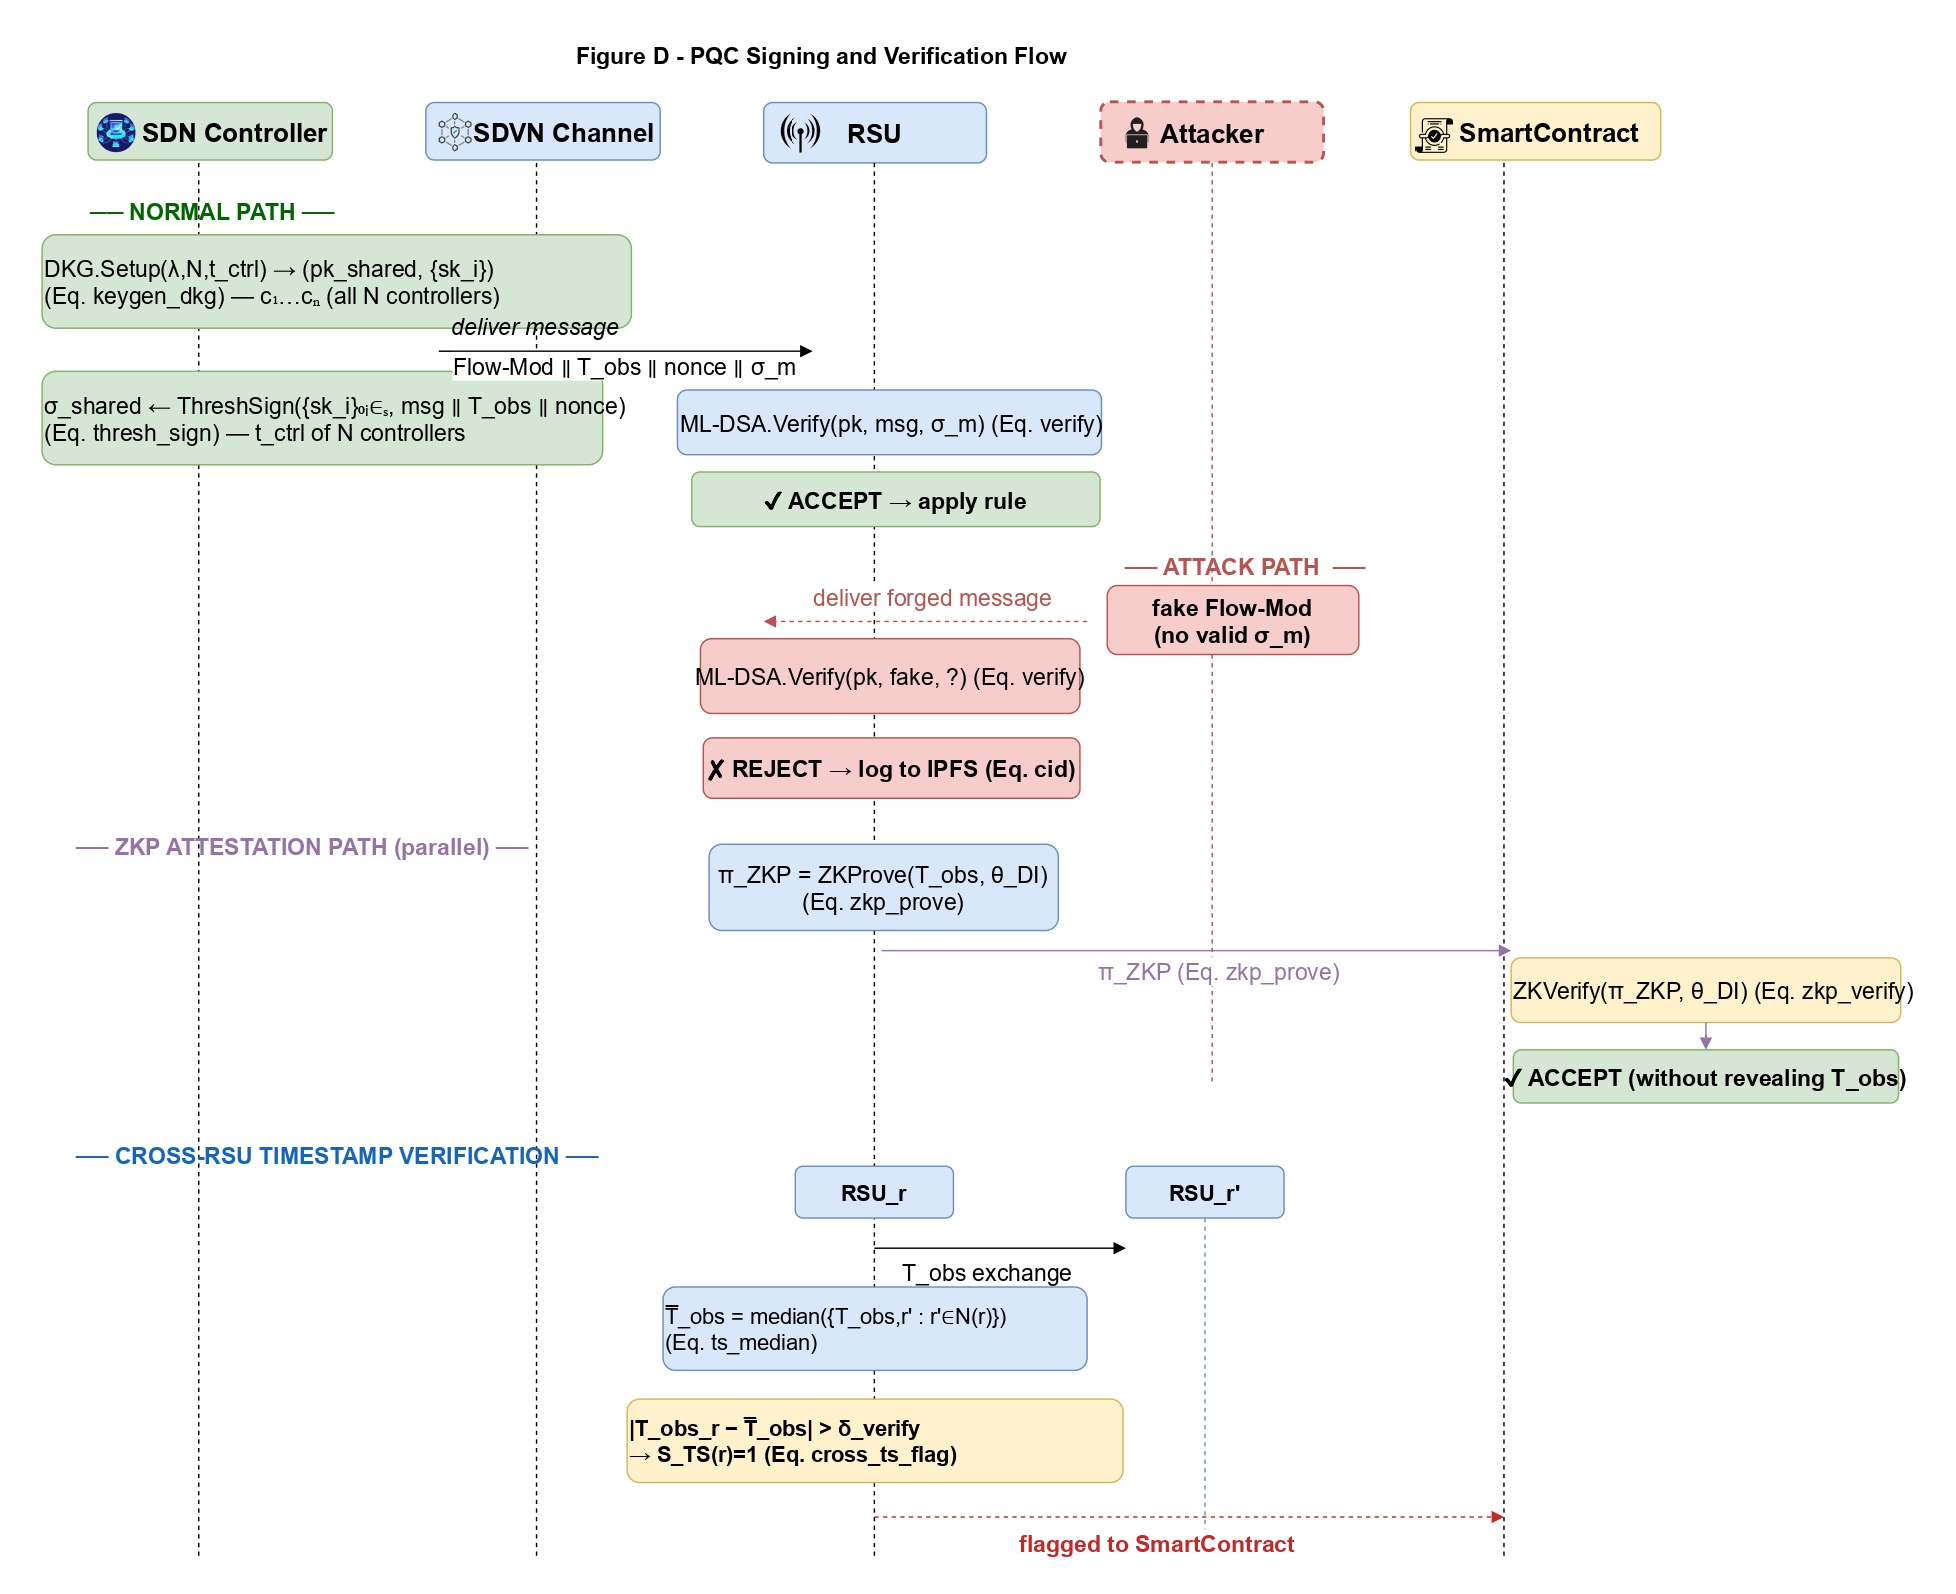
\includegraphics[width=\linewidth]{Progress_Works/DMAP_SDVN/Figure_D_Correct.jpg}
\caption{PQC signing and verification flow using ML-DSA.}
\label{fig:pqc_flow}
\end{figure}
\FloatBarrier
% ====== END FIGURE D ======


As shown in Figure~\ref{fig:pqc_flow}, the Normal Path
authenticates each Flow-Mod via ML-DSA signing and
verification, the Attack Path causes immediate rejection and
IPFS-logged evidence when $\sigma_m$ is invalid, and the ZKP
Attestation Path allows RSUs to prove timing compliance
without revealing the exact observed timestamp
$T_{\mathrm{obs}}^{ij}$, closing the secondary side-channel
leakage path.


\textbf{Lightweight Cryptographic Fallback.}
In LW mode, ML-DSA signatures are replaced by HMAC-SHA-256
authentication tags~\eqref{eq:hmac}, reducing cryptographic overhead
by approximately $40\times$ while maintaining integrity protection
against external attackers. Threshold signatures and ZKP are
suspended in LW mode; their absence is reflected in the reduced
trust-score update sensitivity during lightweight operation.

\begin{comment}
...
\end{comment}

\subsubsection{LLM-Based Contextual Intelligence Module}
\label{sec:llm}

The LLM module serves two formally distinct roles in DMAP-SDVN:
a \emph{real-time contextual scoring} role that augments the DRL
state vector with semantic threat context, and an \emph{offline
forensic analysis} role that interprets blockchain-anchored timing
logs and generates human-readable incident reports. Both roles
operate on a structured representation of the SDVN timing event
log.

\textbf{Timing Log Tokenisation.}
At each epoch $t$, the raw timing event sequence from RSU $r$
is structured into a fixed-length token sequence, as defined
in Equation~\eqref{eq:llm_input}.
\begin{equation}
\mathbf{X}_t^r = \bigl[
  x_1^r, x_2^r, \ldots, x_L^r
\bigr],
\quad
x_l^r = \bigl(
  \Delta\tau_l,\;
  \mathrm{type}_l,\;
  \psi_r^{(l)},\;
  \xi_k^{(l)},\;
  \mathrm{flag}_l
\bigr),
\label{eq:llm_input}
\end{equation}
As shown in Equation~\eqref{eq:llm_input}, $L$ is the context
window length, $\Delta\tau_l$ is the timing deviation of event
$l$, $\mathrm{type}_l \in \{\mathrm{FlowMod},
\mathrm{PacketIn}, \mathrm{LinkEvent}, \mathrm{Beacon}\}$ is
the event category, $\psi_r^{(l)}$ is the RSU trust score at
event $l$, $\xi_k^{(l)}$ is the associated vehicle mobility
state, and $\mathrm{flag}_l \in \{0,1\}$ is the lightweight
signature detection output from Algorithm~\ref{alg:lw}. The sequence $\mathbf{X}_t^r$ is projected into the LLM
embedding space via a learned linear projection $\mathbf{W}_e$,
as defined in Equation~\eqref{eq:llm_encode}.
\begin{equation}
\mathbf{H}_t^r = \mathrm{LLM\_Encoder}
  \bigl(\mathbf{W}_e\,\mathbf{X}_t^r\bigr)
  \in \mathbb{R}^{L \times d_h},
\label{eq:llm_encode}
\end{equation}
As shown in Equation~\eqref{eq:llm_encode}, $d_h$ is the
hidden dimension of the LLM and $\mathbf{H}_t^r$ is the
resulting sequence of contextual hidden states.

\textbf{Real-Time Semantic Anomaly Score.}
A pooling operation over the final hidden states produces a
per-epoch semantic anomaly score for each RSU, as defined in
Equation~\eqref{eq:llm_score}.
\begin{equation}
\lambda_t^r = \sigma\!\left(
  \mathbf{w}_a^\top \cdot
  \frac{1}{L}\sum_{l=1}^{L} \mathbf{H}_t^r[l]
  + b_a
\right) \in [0,1],
\label{eq:llm_score}
\end{equation}
As shown in Equation~\eqref{eq:llm_score}, $\sigma(\cdot)$
is the sigmoid function, and $\mathbf{w}_a$ and $b_a$ are
learned parameters fine-tuned on SDVN timing attack logs. A score $\lambda_t^r$ close to 1 indicates
strong semantic evidence of attack behaviour; close to 0
indicates benign or congestion-like patterns.

\textbf{Contextual Threat Classification.}
Beyond the binary anomaly score, the LLM classifies each timing anomaly into one of four
semantic categories, as defined in
Equation~\eqref{eq:llm_classify}.
\begin{equation}
\hat{c}_t^r = \arg\max_{c\,\in\,\mathcal{C}}
  \;p\!\left(c \mid \mathbf{H}_t^r;\,\theta_{\mathrm{LLM}}\right),
\label{eq:llm_classify}
\end{equation}
As shown in Equation~\eqref{eq:llm_classify}, $\mathcal{C} =
\{\mathrm{congestion},\, \mathrm{attack\text{-}DI},\,
\mathrm{attack\text{-}RC},\, \mathrm{attack\text{-}SC},\,
\mathrm{attack\text{-}SE}\}$ is the set of semantic categories
and $\theta_{\mathrm{LLM}}$ are the fine-tuned LLM parameters.
This five-way classification distinguishes mobility-induced
congestion from each of the four targeted attack variants,
resolving the ambiguity that purely statistical detectors
cannot resolve under high-mobility conditions.

\textbf{LLM Context Vector for DRL Integration.}
The LLM semantic anomaly score and classification logits are
concatenated into a context vector that is fed back into the
DRL state vector~\eqref{eq:state} as the component
$\mathbf{h}_t^{\mathrm{ctx}}$, as defined in
Equation~\eqref{eq:llm_ctx}.
\begin{equation}
\mathbf{h}_t^{\mathrm{ctx}} = \bigl[
  \lambda_t^{r_1}, \ldots, \lambda_t^{r_{|\mathcal{V}_r|}},\;
  \hat{\mathbf{p}}_t^{r_1}, \ldots,
  \hat{\mathbf{p}}_t^{r_{|\mathcal{V}_r|}}
\bigr],
\label{eq:llm_ctx}
\end{equation}
As shown in Equation~\eqref{eq:llm_ctx}, $\hat{\mathbf{p}}_t^r
= p(c \mid \mathbf{H}_t^r;\theta_{\mathrm{LLM}}) \in
\mathbb{R}^{|\mathcal{C}|}$ is the softmax probability vector
over attack categories for RSU $r$. This coupling
means the DRL agent's action selection is informed by the
LLM's semantic understanding of the timing log, enabling it
to distinguish congestion-driven timing deviations from
genuine attacks and avoid false-positive quarantine actions.


\begin{comment}
\textbf{Offline Forensic Report Generation.}
In offline mode, the LLM operates on the full IPFS-anchored
commitment sequence retrieved from the blockchain. Define the
offline input as the concatenation of all epoch-level token
sequences over an investigation window $[t_1, t_2]$:
\begin{equation}
\mathbf{X}_{\mathrm{off}}^r =
  \bigl[\mathbf{X}_{t_1}^r,\;
  \mathbf{X}_{t_1+1}^r,\;\ldots,\;
  \mathbf{X}_{t_2}^r\bigr].
\label{eq:llm_offline_input}
\end{equation}
The LLM generates a structured natural-language forensic
report $\mathcal{R}$ conditioned on this sequence:
\begin{equation}
\mathcal{R} = \mathrm{LLM\_Generate}\!\left(
  \mathbf{X}_{\mathrm{off}}^r;\;
  \mathcal{P}_{\mathrm{forensic}}
\right),
\label{eq:llm_report}
\end{equation}
where $\mathcal{P}_{\mathrm{forensic}}$ is a structured
forensic prompt template specifying the report format:
attack type, affected RSUs, timing deviation statistics,
mobility context, and recommended remediation actions.
The report $\mathcal{R}$ is cryptographically signed by the
controller using ML-DSA~\eqref{eq:sign} before being stored
as a final IPFS-anchored blockchain record, ensuring
forensic non-repudiation.

\textbf{Implementation.}
The LLM module is implemented using Hugging Face Transformers
with a fine-tuned compact decoder model (e.g.,
Mistral-7B-Instruct or equivalent) adapted for structured
network log analysis. Fine-tuning is performed on NS3-generated
SDVN timing attack logs using supervised instruction tuning
with attack-label annotations. The projection layer
$\mathbf{W}_e$, anomaly head $(\mathbf{w}_a, b_a)$, and
classification head are trained end-to-end with the LLM
backbone frozen, reducing fine-tuning cost while preserving
language understanding capabilities.
\end{comment}


\textbf{Offline Forensic Report Generation.}
In offline mode, the LLM operates on the full IPFS-anchored
commitment sequence retrieved from the blockchain. The offline
input is defined as the concatenation of all epoch-level token
sequences over an investigation window $[t_1, t_2]$, as given
in Equation~\eqref{eq:llm_offline_input}.
\begin{equation}
\mathbf{X}_{\mathrm{off}}^r =
  \bigl[\mathbf{X}_{t_1}^r,\;
  \mathbf{X}_{t_1+1}^r,\;\ldots,\;
  \mathbf{X}_{t_2}^r\bigr],
\label{eq:llm_offline_input}
\end{equation}
As shown in Equation~\eqref{eq:llm_offline_input},
$\mathbf{X}_{t}^r$ is the structured token sequence for RSU $r$
at epoch $t$ as defined in~\eqref{eq:llm_input},
$t_1$ and $t_2$ denote the start and end of the forensic
investigation window, and the concatenation spans all epochs
in $[t_1, t_2]$ to provide the LLM with the full temporal
context of the incident.
The LLM then generates a structured natural-language forensic
report $\mathcal{R}$ conditioned on this offline input
sequence, as expressed in Equation~\eqref{eq:llm_report}.
\begin{equation}
\mathcal{R} = \mathrm{LLM\_Generate}\!\left(
  \mathbf{X}_{\mathrm{off}}^r;\;
  \mathcal{P}_{\mathrm{forensic}}
\right),
\label{eq:llm_report}
\end{equation}
As shown in Equation~\eqref{eq:llm_report},
$\mathbf{X}_{\mathrm{off}}^r$ is the concatenated offline
input from~\eqref{eq:llm_offline_input} and
$\mathcal{P}_{\mathrm{forensic}}$ is a structured forensic
prompt template specifying the report format, covering attack
type, affected RSUs, timing deviation statistics, mobility
context, and recommended remediation actions. The generated
report $\mathcal{R}$ is cryptographically signed by the
controller using ML-DSA~\eqref{eq:sign} before being stored
as a final IPFS-anchored blockchain record, ensuring
forensic non-repudiation.

\begin{comment}
\textbf{Implementation.}
The LLM module is implemented using Hugging Face Transformers
with a fine-tuned compact decoder model (e.g.,
Mistral-7B-Instruct or equivalent) adapted for structured
network log analysis. Fine-tuning is performed on NS3-generated
SDVN timing attack logs using supervised instruction tuning
with attack-label annotations. The projection layer
$\mathbf{W}_e$, anomaly head $(\mathbf{w}_a, b_a)$, and
classification head are trained end-to-end with the LLM
backbone frozen, reducing fine-tuning cost while preserving
language understanding capabilities.



FIND THIS EXACT TEXT (search in Overleaf using Ctrl+F):
language understanding capabilities.
That is the very last line of Section 3.6.4 (LLM-Based Contextual Intelligence Module), ending the Implementation paragraph.

BEFORE (what is there now):
latexThe projection layer
$\mathbf{W}_e$, anomaly head $(\mathbf{w}_a, b_a)$, and
classification head are trained end-to-end with the LLM
backbone frozen, reducing fine-tuning cost while preserving
language understanding capabilities.
\end{comment}
\begin{comment}
...
\end{comment}

% \subsection{Defence Algorithms}

The projection layer
$\mathbf{W}_e$, anomaly head $(\mathbf{w}_a, b_a)$, and
classification head are trained end-to-end with the LLM
backbone frozen, reducing fine-tuning cost while preserving
language understanding capabilities.


Algorithm~\ref{alg:llm} implements the LLM module
covering both real-time contextual scoring and offline
forensic report generation.

\begin{algorithm}[H]
\caption{LLM Contextual Intelligence (\texttt{LLM-Intel})}
\label{alg:llm}
\begin{algorithmic}[1]
\small
\Procedure{\texttt{LLM-RealTime}}
  {$\mathbf{X}_t^r,\,\theta_{\mathrm{LLM}},\,\mathbf{W}_e$}
  \State $\mathbf{H}_t^r \gets
    \mathrm{LLM\_Encoder}(\mathbf{W}_e\,\mathbf{X}_t^r)$
  \State $\lambda_t^r \gets
    \sigma(\mathbf{w}_a^\top
    \tfrac{1}{L}\sum_l \mathbf{H}_t^r[l] + b_a)$
  \State $\hat{c}_t^r \gets
    \arg\max_c\;p(c\mid\mathbf{H}_t^r;\theta_{\mathrm{LLM}})$
  \State $\hat{\mathbf{p}}_t^r \gets
    \mathrm{softmax}(\mathrm{logits}
    (c\mid\mathbf{H}_t^r))$
  \State \textbf{return}
    $(\lambda_t^r,\,\hat{c}_t^r,\,\hat{\mathbf{p}}_t^r)$
\EndProcedure
\vspace{0.4em}
\Procedure{\texttt{LLM-Offline}}
  {$\mathbf{X}_{\mathrm{off}}^r,\,
  \mathcal{P}_{\mathrm{forensic}},\,
  \mathrm{sk}_{\mathrm{ctrl}}$}
  \State $\mathcal{R} \gets
    \mathrm{LLM\_Generate}(
    \mathbf{X}_{\mathrm{off}}^r;\,
    \mathcal{P}_{\mathrm{forensic}})$
  \State $\sigma_\mathcal{R} \gets
    \mathrm{ML\text{-}DSA.Sign}
    (\mathrm{sk}_{\mathrm{ctrl}},\mathcal{R})$
  \State $\mathrm{CID}_\mathcal{R} \gets
    \mathrm{IPFS\_Store}
    (\mathcal{R}\;\|\;\sigma_\mathcal{R})$
  \State \texttt{SmartContract.RecordReport}
    $(\mathrm{CID}_\mathcal{R})$
  \State \textbf{return}
    $(\mathcal{R},\,\mathrm{CID}_\mathcal{R})$
\EndProcedure
\end{algorithmic}
\end{algorithm}

As shown in Algorithm~\ref{alg:llm}, the
\texttt{LLM-RealTime} procedure runs at every epoch per
RSU, producing the semantic anomaly score $\lambda_t^r$
and the attack-category probability vector
$\hat{\mathbf{p}}_t^r$ which feed into the DRL state
vector $\mathbf{h}_t^{\mathrm{ctx}}$. The
\texttt{LLM-Offline} procedure is invoked post-incident,
generating a structured forensic report $\mathcal{R}$
that is ML-DSA signed and stored as a final blockchain
record, ensuring forensic non-repudiation.

% ====== FIGURE F — CORRECTED ======

The LLM module architecture is illustrated in
Figure~\ref{fig:llm_arch}. The input zone (left) receives
five context sources traffic logs, mobility context
$\varphi_{\mathrm{DI}} \to \varphi_{\mathrm{SC}}$, threat
intelligence feeds, historical incidents, and operator
queries that feed into two parallel processing paths.

The real-time path (\textsc{LLM-RealTime}, left sub-zone)
passes inputs through a context embedding encoder and
attention layers~\eqref{eq:llm_encode}, producing a
Scoring Head that computes the semantic anomaly score
$\lambda_t^r \in [0,1]$~\eqref{eq:llm_score}. The context
vector $\mathbf{h}^{\mathrm{ctx}}$~\eqref{eq:llm_ctx} is
fed upward (purple dashed arrow) into the DRL agent state
$\mathbf{s}_t$~\eqref{eq:state} for real-time augmentation.

The offline path (\textsc{LLM-Intel}, right sub-zone)
processes the full IPFS commitment sequence through a
Sequence Model (Transformer)~\eqref{eq:llm_encode}, a
Reasoning Layer applying five-way chain-of-thought
classification~\eqref{eq:llm_classify}, and a Report
Generator that produces the forensic incident report
$\mathcal{R}$~\eqref{eq:llm_report}.

The output zone (right) shows three consumers: the DRL
Agent receives $\mathbf{h}^{\mathrm{ctx}}$~\eqref{eq:llm_ctx}
for state augmentation, the Operator Dashboard receives
real-time alerts from the classification
head~\eqref{eq:llm_classify}, and the Blockchain Audit
Logs receive the PQC-signed incident report
$\mathcal{R}$ anchored via
IPFS~\eqref{eq:cid}--\eqref{eq:block}.

\begin{figure}[htb]
\centering
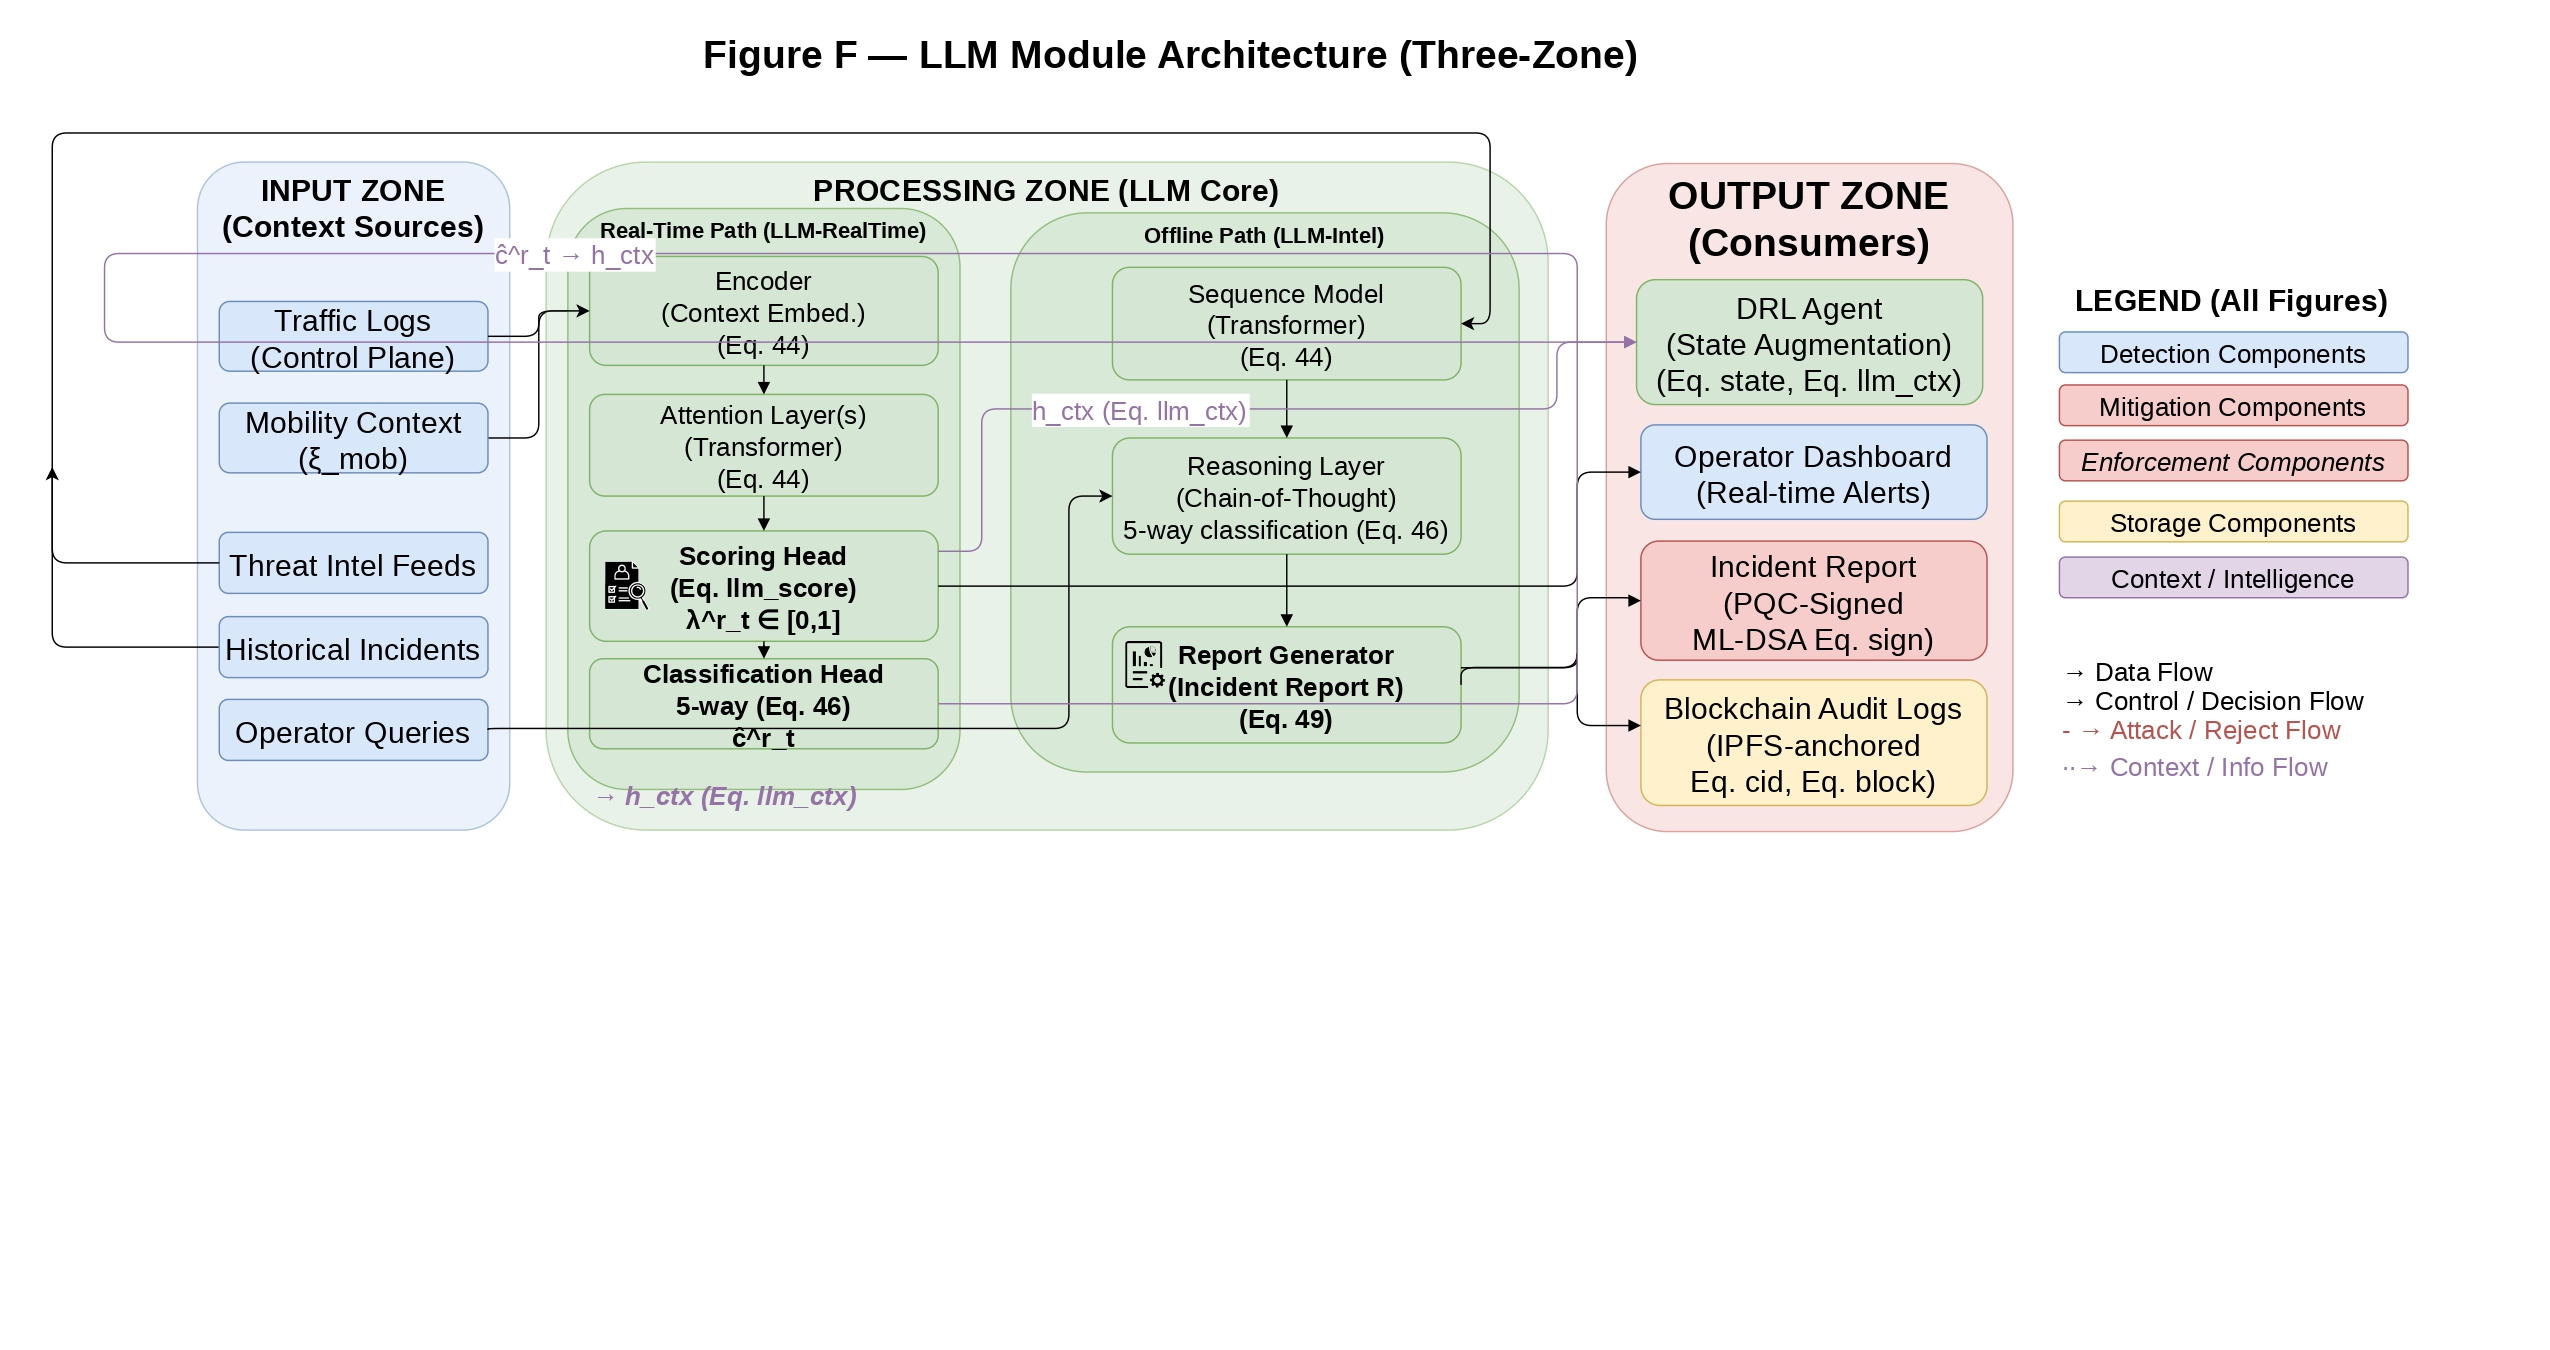
\includegraphics[width=1.2\linewidth]{Progress_Works/DMAP_SDVN/Figure_F.jpg}
\caption{LLM module architecture showing real-time and offline processing paths.}
\label{fig:llm_arch}
\end{figure}
\FloatBarrier
% ====== END FIGURE F ======


As shown in Figure~\ref{fig:llm_arch}, the real-time path
produces the semantic anomaly score $\lambda_t^r$ and context
vector $\mathbf{h}^{\mathrm{ctx}}$ that feeds into the DRL
agent state, while the offline path processes the full IPFS
commitment sequence through a Transformer sequence model and
reasoning layer to generate the PQC-signed forensic report
$\mathcal{R}$ anchored to the blockchain audit log.

\subsubsection{Per-Variant Detection and Mitigation Algorithms}
\label{sec:per_variant}

Having defined the DRL detection agent (Section~\ref{sec:drl})
and the blockchain smart-contract enforcement layer
(Section~\ref{sec:blockchain}), we now present the four
per-variant detection and mitigation algorithms that integrate
both components. Each algorithm operates in either Lightweight
(LW) or Full mode according to the switching policy
in~\eqref{eq:mode_switch}, applying the appropriate subset of
authentication, DRL inference, and blockchain anchoring steps.

Algorithm~\ref{alg:di} presents the full detection and
mitigation cycle for Delay Injection attacks, combining
HMAC and ML-DSA authentication, mobility-adapted threshold
detection, ZKP proof generation, IPFS anchoring, and
DRL-guided mitigation action selection.

\begin{algorithm}[H]
\caption{Delay Injection Detection and Mitigation
(\texttt{DI-Defend})}
\label{alg:di}
\begin{algorithmic}[1]
\small
\Procedure{\texttt{DI-Defend}}
  {$m,\hat{v}_k,\mathrm{mode},\pi_\theta,\mathrm{sk}_{\mathrm{ctrl}}$}
  \State \textbf{--- Authentication ---}
  \State Verify $\tau_{\mathrm{HMAC}}(m)$~\eqref{eq:hmac};
    \textbf{if} invalid \textbf{then return} \textsc{Reject}
  \State Verify $\mathrm{ML\text{-}DSA.Verify}
    (\mathrm{pk}_{\mathrm{ctrl}},m,\sigma_m)$~\eqref{eq:verify};
    \textbf{if} invalid \textbf{then return} \textsc{Reject}
  \State Check nonce freshness and TTL;
    \textbf{if} expired \textbf{then return} \textsc{Reject}
  \State \textbf{--- Delay Detection ---}
  \State $\Delta\tau \gets T_{\mathrm{obs}}^m - T_{\mathrm{exp}}^m$
    \Comment{from~\eqref{eq:expected}}
  \State $\theta_{DI} \gets \tau_{\mathrm{TTL}}
    (1+\alpha_{DI}\hat{v}_k/v_{\max})-\epsilon_0$
    \Comment{from~\eqref{eq:theta_di}}
  \State $S_{DI} \gets \mathbb{1}[\Delta\tau > \theta_{DI}]$
    \Comment{from~\eqref{eq:sig_di}}
  \If{$S_{DI}=0$}
    \State Accept $m$; update $\psi_r \uparrow$~\eqref{eq:trust_update}
    \State \textbf{return} \textsc{Benign}
  \EndIf
  \State \textbf{--- Mode-Dependent Mitigation ---}
  \If{$\mathrm{mode} = \mathrm{LW}$}
    \State Discard $m$; log locally;
      decrement $\psi_r \gets \psi_r - \Delta_{\mathrm{penalty}}$
    \State \textbf{return} $(\textsc{Attack},\mathrm{DI},\Delta\tau)$
  \EndIf
  \State \textbf{--- Full Mode: DRL + Blockchain ---}
  \State $\pi_{\mathrm{ZKP}} \gets \mathrm{ZKProve}
    (T_{\mathrm{obs}}^m, \theta_{DI})$~\eqref{eq:zkp_prove}
  \State $C_m \gets \mathrm{Hash}
    (m\|\Delta\tau\|\pi_{\mathrm{ZKP}}\|\sigma_m)$
    \Comment{from~\eqref{eq:commitment}}
  \State $\mathrm{CID} \gets \mathrm{IPFS\_Store}(C_m)$
    \Comment{from~\eqref{eq:cid}}
  \State \texttt{SmartContract.SubmitTimingProof}
    $(r,C_m,\sigma_r)$
  \State $\mathbf{s}_t \gets \texttt{BuildState}
    (\Delta\tau,\boldsymbol{\psi},\boldsymbol{\xi},
    \mathbf{h}^{\mathrm{ctx}})$~\eqref{eq:state}
  \State $a_t \gets \pi_\theta(\mathbf{s}_t)$
    \Comment{from~\eqref{eq:actions}}
  \If{$a_t \in \{a_2^{\mathrm{isolate}},a_3^{\mathrm{reroute}}\}$}
    \State \texttt{PQC-Mitigate}$(r,\mathrm{DI},
      \mathrm{sk}_{\mathrm{ctrl}})$
  \EndIf
  \State \textbf{return} $(\textsc{Attack},\mathrm{DI},
    a_t,\mathrm{CID})$
\EndProcedure
\end{algorithmic}
\end{algorithm}

As shown in Algorithm~\ref{alg:di}, the procedure begins
with HMAC and ML-DSA authentication before any timing
analysis, ensuring unsigned or replayed messages are
rejected immediately. In LW mode, a confirmed delay
deviation above $\theta_{\mathrm{DI}}$ causes local
message rejection and trust decrement with no blockchain
overhead. In Full mode, a ZKP proof is generated, the
commitment is anchored to IPFS, and the DRL agent selects
an action from isolate, reroute, or strict verification.

Algorithm~\ref{alg:rc} handles race condition exploitation
by detecting contradictory event pairs and enforcing atomic
flow-rule update semantics via smart contracts in Full mode.

\begin{algorithm}[H]
\caption{Race Condition Detection and Mitigation
(\texttt{RC-Defend})}
\label{alg:rc}
\begin{algorithmic}[1]
\small
\Procedure{\texttt{RC-Defend}}
  {$e_{\mathrm{new}},\mathcal{Q},\mathrm{mode},
  \pi_\theta,\mathrm{sk}_{\mathrm{ctrl}}$}
  \State Append $e_{\mathrm{new}}$ to event queue $\mathcal{Q}$
  \For{each $e_{\mathrm{prev}} \in \mathcal{Q}$
    from $\mathrm{src}(e_{\mathrm{new}})$}
    \State $\mathcal{C} \gets
      \mathrm{ConflictCheck}(e_{\mathrm{prev}},e_{\mathrm{new}})$
    \State $\Delta t \gets |t_{e_{\mathrm{new}}}
      - t_{e_{\mathrm{prev}}}|$
    \If{$\mathcal{C}=-1$
        \textbf{and} $\Delta t < \epsilon_{RC}$}
      \State $S_{RC} \gets 1$; break
    \EndIf
  \EndFor
  \If{$S_{RC}=0$}
    \State \textbf{return} \textsc{Benign}
  \EndIf
  \If{$\mathrm{mode} = \mathrm{LW}$}
    \State Hold both conflicting Flow-Mods;
      request re-report from RSU
    \State $\psi_r \gets \psi_r - \Delta_{\mathrm{penalty}}$
    \State \textbf{return}
      $(\textsc{Attack},\mathrm{RC},e_{\mathrm{prev}},
      e_{\mathrm{new}})$
  \EndIf
  \State $\mathbf{s}_t \gets \texttt{BuildState}
    (\Delta\tau^{RC},\boldsymbol{\psi},\boldsymbol{\xi},
    \mathbf{h}^{\mathrm{ctx}})$~\eqref{eq:state}
  \State $a_t \gets \pi_\theta(\mathbf{s}_t)$
  \If{$a_t = a_1^{\mathrm{verify}}$}
    \State Query neighbouring RSUs for consensus
  \ElsIf{$a_t \in
    \{a_2^{\mathrm{isolate}},a_4^{\mathrm{strict}}\}$}
    \State \texttt{SmartContract.EnforceAtomicUpdate}
      $(r,e_{\mathrm{prev}},e_{\mathrm{new}})$
    \State \texttt{PQC-Mitigate}$(r,\mathrm{RC},
      \mathrm{sk}_{\mathrm{ctrl}})$
  \EndIf
  \State $\mathrm{CID} \gets \mathrm{IPFS\_Store}
    (\mathrm{Hash}(e_{\mathrm{prev}}\|e_{\mathrm{new}}\|\Delta t))$
  \State \textbf{return}
    $(\textsc{Attack},\mathrm{RC},a_t,\mathrm{CID})$
\EndProcedure
\end{algorithmic}
\end{algorithm}

As shown in Algorithm~\ref{alg:rc}, each incoming event
is compared against prior events from the same RSU. When
a conflicting pair satisfying $\mathcal{C}=-1$ is found
within the race window $\epsilon_{\mathrm{RC}}$, the
signature fires. In LW mode both conflicting Flow-Mods
are held and a re-report is requested. In Full mode the
DRL agent queries neighbouring RSUs for consensus or
invokes the smart contract to enforce atomic update
semantics.

Algorithm~\ref{alg:sc_def} addresses timing side-channel
attacks by computing correlation-based signatures over a
sliding observation window and applying channel obfuscation
as an immediate preventive action in both modes.

\begin{algorithm}[H]
\caption{Timing Side-Channel Detection and Mitigation
(\texttt{SC-Defend})}
\label{alg:sc_def}
\begin{algorithmic}[1]
\small
\Procedure{\texttt{SC-Defend}}
  {$\mathbf{T}_{1:n},\mathbf{E}_{1:n},\mathrm{mode},
  \pi_\theta,\mathrm{sk}_{\mathrm{ctrl}}$}
  \State $\hat{\rho} \gets
    \mathrm{PearsonCorr}(\mathbf{T}_{1:n},\mathbf{E}_{1:n})$
  \State $\hat{\sigma}_{\mathrm{timing}} \gets
    \mathrm{std}(\mathbf{T}_{1:n})$
  \State $S_{SC} \gets
    \mathbb{1}[\hat{\rho}>\rho_{th}]
    \cdot\mathbb{1}
    [\hat{\sigma}_{\mathrm{timing}}<\theta_{\mathrm{noise}}]$
    \Comment{from~\eqref{eq:sig_sc}}
  \If{$S_{SC}=0$}
    \State \textbf{return} \textsc{Benign}
  \EndIf
  \State Inject noise $\eta \sim
    \mathcal{U}(0,\epsilon_{\mathrm{noise}})$;
    enforce encrypted channels
  \If{$\mathrm{mode} = \mathrm{LW}$}
    \State Log $(\hat{\rho},\hat{\sigma})$; flag RSU
    \State \textbf{return}
      $(\textsc{Attack},\mathrm{SC},\hat{\rho})$
  \EndIf
  \State Switch RSU attestations to ZKP mode~\eqref{eq:zkp_prove}
  \State $\mathbf{s}_t \gets \texttt{BuildState}
    (\hat{\rho},\boldsymbol{\psi},\boldsymbol{\xi},
    \mathbf{h}^{\mathrm{ctx}})$~\eqref{eq:state}
  \State $a_t \gets \pi_\theta(\mathbf{s}_t)$
  \If{$a_t \in
    \{a_2^{\mathrm{isolate}},a_4^{\mathrm{strict}}\}$}
    \State \texttt{PQC-Mitigate}$(r,\mathrm{SC},
      \mathrm{sk}_{\mathrm{ctrl}})$
  \EndIf
  \State $\mathrm{CID} \gets \mathrm{IPFS\_Store}
    (\mathrm{Hash}(\hat{\rho}\|\hat{\sigma}\|
    \mathbf{T}_{1:n}))$
  \State \textbf{return}
    $(\textsc{Attack},\mathrm{SC},a_t,\mathrm{CID})$
\EndProcedure
\end{algorithmic}
\end{algorithm}

As shown in Algorithm~\ref{alg:sc_def}, both the Pearson
correlation and the timing standard deviation must
simultaneously exceed their thresholds before the
signature fires, reducing false positives from
congestion-induced correlation. An immediate preventive
action --- injection of calibrated timing noise and
enforcement of encrypted channels --- is applied in both
modes. In Full mode, ZKP attestation mode is additionally
activated so that RSUs never reveal exact timestamps
during the probationary period.

Algorithm~\ref{alg:se} addresses synchronisation exploits
by monitoring beacon inter-arrival patterns and handover
report timing differentials, with mobility-aware thresholds
to avoid false positives during legitimate handovers.

\begin{algorithm}[H]
\caption{Synchronisation Exploit Detection and Mitigation
(\texttt{SE-Defend})}
\label{alg:se}
\begin{algorithmic}[1]
\small
\Procedure{\texttt{SE-Defend}}
  {$\mathbf{b}_{1:n},\mathbf{R}_t,\mathrm{mode},
  \pi_\theta,\mathrm{sk}_{\mathrm{ctrl}}$}
  \State $\mathrm{gap} \gets
    \exists\,k:\;b_k > 2/f_{\mathrm{beacon}}$
  \State $\mathrm{var} \gets
    \frac{1}{n}\sum_{i=1}^{n}(b_i-\bar{b})^2$
  \State $S_{SE}^{\mathrm{beacon}} \gets
    \mathbb{1}[\mathrm{gap}]
    \cdot\mathbb{1}[\mathrm{var}>\theta_{SE}^2]$
  \State $\Delta\tau_{\mathrm{HO}} \gets
    |T_{\mathrm{report}}^{r_A} - T_{\mathrm{report}}^{r_B}|$
  \State $S_{SE} \gets S_{SE}^{\mathrm{beacon}}
    \vee \mathbb{1}[\Delta\tau_{\mathrm{HO}} >
    \theta_{\mathrm{HO}}(\hat{v}_k)]$
  \If{$S_{SE}=0$}
    \State \textbf{return} \textsc{Benign}
  \EndIf
  \If{$\mathrm{mode} = \mathrm{LW}$}
    \State Require 3 consecutive valid beacons
      before handover commit
    \State $\psi_r \gets \psi_r - \Delta_{\mathrm{penalty}}$
    \State \textbf{return}
      $(\textsc{Attack},\mathrm{SE},\mathrm{var},
      \Delta\tau_{\mathrm{HO}})$
  \EndIf
  \State Validate vehicle trajectory plausibility
  \State Request corroboration from $\geq t$ RSUs
  \State $\mathbf{s}_t \gets \texttt{BuildState}
    (\Delta b,\boldsymbol{\psi},\boldsymbol{\xi},
    \mathbf{h}^{\mathrm{ctx}})$~\eqref{eq:state}
  \State $a_t \gets \pi_\theta(\mathbf{s}_t)$
  \If{$a_t \in
    \{a_2^{\mathrm{isolate}},a_3^{\mathrm{reroute}}\}$}
    \State \texttt{PQC-Mitigate}$(r,\mathrm{SE},
      \mathrm{sk}_{\mathrm{ctrl}})$
  \EndIf
  \State $\mathrm{CID} \gets \mathrm{IPFS\_Store}
    (\mathrm{Hash}(\mathrm{var}\|\Delta\tau_{\mathrm{HO}}))$
  \State \textbf{return}
    $(\textsc{Attack},\mathrm{SE},a_t,\mathrm{CID})$
\EndProcedure
\end{algorithmic}
\end{algorithm}

As shown in Algorithm~\ref{alg:se}, the beacon check and
handover timing differential check are evaluated
independently and combined with logical OR, so either
condition alone triggers detection. In LW mode, a
hysteresis guard requiring three consecutive valid beacons
prevents oscillation attacks from causing repeated
unnecessary handovers. In Full mode, the DRL agent
validates the vehicle trajectory and requests
threshold-signed corroboration from neighbouring RSUs
before committing a handover decision.


\begin{comment}
...
\end{comment}


\begin{comment}
\subsection{Per-Variant Detection and Mitigation Algorithms}
Algorithm~\ref{alg:di} covers the full detection and mitigation
cycle for delay injection attacks, operating in both LW and Full
modes. In LW mode, HMAC verification and threshold comparison
provide immediate rejection; in Full mode, the DRL agent and
smart contract provide adaptive enforcement.

\begin{algorithm}[H]
\caption{Delay Injection Detection and Mitigation
(\texttt{DI-Defend})}
\label{alg:di}
\begin{algorithmic}[1]
\small
\Procedure{\texttt{DI-Defend}}
  {$m,\hat{v}_k,\mathrm{mode},\pi_\theta,\mathrm{sk}_{\mathrm{ctrl}}$}
  \State \textbf{--- Authentication ---}
  \State Verify $\tau_{\mathrm{HMAC}}(m)$~\eqref{eq:hmac};
    \textbf{if} invalid \textbf{then return} \textsc{Reject}
  \State Verify $\mathrm{ML\text{-}DSA.Verify}
    (\mathrm{pk}_{\mathrm{ctrl}},m,\sigma_m)$~\eqref{eq:verify};
    \textbf{if} invalid \textbf{then return} \textsc{Reject}
  \State Check nonce freshness and TTL;
    \textbf{if} expired \textbf{then return} \textsc{Reject}
  \State \textbf{--- Delay Detection ---}
  \State $\Delta\tau \gets T_{\mathrm{obs}}^m - T_{\mathrm{exp}}^m$
    \Comment{from~\eqref{eq:expected}}
  \State $\theta_{DI} \gets \tau_{\mathrm{TTL}}
    (1+\alpha_{DI}\hat{v}_k/v_{\max})-\epsilon_0$
    \Comment{from~\eqref{eq:theta_di}}
  \State $S_{DI} \gets \mathbb{1}[\Delta\tau > \theta_{DI}]$
    \Comment{from~\eqref{eq:sig_di}}
  \If{$S_{DI}=0$}
    \State Accept $m$; update $\psi_r \uparrow$~\eqref{eq:trust_update}
    \State \textbf{return} \textsc{Benign}
  \EndIf
  \State \textbf{--- Mode-Dependent Mitigation ---}
  \If{$\mathrm{mode} = \mathrm{LW}$}
    \State Discard $m$; log locally;
      decrement $\psi_r \gets \psi_r - \Delta_{\mathrm{penalty}}$
    \State \textbf{return} $(\textsc{Attack},\mathrm{DI},\Delta\tau)$
  \EndIf
  \State \textbf{--- Full Mode: DRL + Blockchain ---}
  \State $\pi_{\mathrm{ZKP}} \gets \mathrm{ZKProve}
    (T_{\mathrm{obs}}^m, \theta_{DI})$~\eqref{eq:zkp_prove}
  \State $C_m \gets \mathrm{Hash}
    (m\|\Delta\tau\|\pi_{\mathrm{ZKP}}\|\sigma_m)$
    \Comment{from~\eqref{eq:commitment}}
  \State $\mathrm{CID} \gets \mathrm{IPFS\_Store}(C_m)$
    \Comment{from~\eqref{eq:cid}}
  \State \texttt{SmartContract.SubmitTimingProof}
    $(r,C_m,\sigma_r)$~\Comment{Alg.~\ref{alg:sc}}
  \State $\mathbf{s}_t \gets \texttt{BuildState}
    (\Delta\tau,\boldsymbol{\psi},\boldsymbol{\xi},
    \mathbf{h}^{\mathrm{ctx}})$~\eqref{eq:state}
  \State $a_t \gets \pi_\theta(\mathbf{s}_t)$
    \Comment{from~\eqref{eq:actions}}
  \If{$a_t \in \{a_2^{\mathrm{isolate}},a_3^{\mathrm{reroute}}\}$}
    \State \texttt{PQC-Mitigate}$(r,\mathrm{DI},
      \mathrm{sk}_{\mathrm{ctrl}})$~\Comment{Alg.~\ref{alg:pqc}}
  \EndIf
  \State \textbf{return} $(\textsc{Attack},\mathrm{DI},
    a_t,\mathrm{CID})$
\EndProcedure
\end{algorithmic}
\end{algorithm}


Algorithm~\ref{alg:rc} handles race condition exploitation
by detecting contradictory event pairs and enforcing atomic
flow-rule update semantics via smart contracts in Full mode.

\begin{algorithm}[H]
\caption{Race Condition Detection and Mitigation
(\texttt{RC-Defend})}
\label{alg:rc}
\begin{algorithmic}[1]
\small
\Procedure{\texttt{RC-Defend}}
  {$e_{\mathrm{new}},\mathcal{Q},\mathrm{mode},
  \pi_\theta,\mathrm{sk}_{\mathrm{ctrl}}$}
  \State \textbf{--- Event Queue Inspection ---}
  \State Append $e_{\mathrm{new}}$ to event queue $\mathcal{Q}$
  \For{each $e_{\mathrm{prev}} \in \mathcal{Q}$
    from $\mathrm{src}(e_{\mathrm{new}})$}
    \State $\mathcal{C} \gets
      \mathrm{ConflictCheck}(e_{\mathrm{prev}},e_{\mathrm{new}})$
      \Comment{from~\eqref{eq:sig_rc}}
    \State $\Delta t \gets |t_{e_{\mathrm{new}}}
      - t_{e_{\mathrm{prev}}}|$
    \If{$\mathcal{C}=-1$
        \textbf{and} $\Delta t < \epsilon_{RC}$}
      \State $S_{RC} \gets 1$; break
    \EndIf
  \EndFor
  \If{$S_{RC}=0$}
    \State Process $e_{\mathrm{new}}$ normally;
      generate Flow-Mod
    \State \textbf{return} \textsc{Benign}
  \EndIf
  \State \textbf{--- Mode-Dependent Mitigation ---}
  \If{$\mathrm{mode} = \mathrm{LW}$}
    \State Hold both conflicting Flow-Mods;
      request re-report from RSU
    \State Decrement
      $\psi_r \gets \psi_r - \Delta_{\mathrm{penalty}}$
    \State \textbf{return}
      $(\textsc{Attack},\mathrm{RC},e_{\mathrm{prev}},
      e_{\mathrm{new}})$
  \EndIf
  \State \textbf{--- Full Mode: Atomic Enforcement ---}
  \State $\mathbf{s}_t \gets \texttt{BuildState}
    (\Delta\tau^{RC},\boldsymbol{\psi},\boldsymbol{\xi},
    \mathbf{h}^{\mathrm{ctx}})$~\eqref{eq:state}
  \State $a_t \gets \pi_\theta(\mathbf{s}_t)$
  \If{$a_t = a_1^{\mathrm{verify}}$}
    \State Query $\geq t$ neighbouring RSUs for
      link-state consensus
    \State Accept majority-consistent event;
      discard outlier
  \ElsIf{$a_t \in
    \{a_2^{\mathrm{isolate}},a_4^{\mathrm{strict}}\}$}
    \State \texttt{SmartContract.EnforceAtomicUpdate}
      $(r,e_{\mathrm{prev}},e_{\mathrm{new}})$
    \State \texttt{PQC-Mitigate}$(r,\mathrm{RC},
      \mathrm{sk}_{\mathrm{ctrl}})$~\Comment{Alg.~\ref{alg:pqc}}
  \EndIf
  \State $C_{RC} \gets \mathrm{Hash}
    (e_{\mathrm{prev}}\|e_{\mathrm{new}}\|\Delta t)$
  \State $\mathrm{CID} \gets \mathrm{IPFS\_Store}(C_{RC})$
  \State \textbf{return}
    $(\textsc{Attack},\mathrm{RC},a_t,\mathrm{CID})$
\EndProcedure
\end{algorithmic}
\end{algorithm}


Algorithm~\ref{alg:sc_def} addresses timing side-channel
attacks by computing correlation-based signatures over a
sliding observation window and applying channel obfuscation
as the primary mitigation in both modes.

\begin{algorithm}[H]
\caption{Timing Side-Channel Detection and Mitigation
(\texttt{SC-Defend})}
\label{alg:sc_def}
\begin{algorithmic}[1]
\small
\Procedure{\texttt{SC-Defend}}
  {$\mathbf{T}_{1:n},\mathbf{E}_{1:n},\mathrm{mode},
  \pi_\theta,\mathrm{sk}_{\mathrm{ctrl}}$}
  \State \textbf{--- Passive Observation Detection ---}
  \State $\hat{\rho} \gets
    \mathrm{PearsonCorr}(\mathbf{T}_{1:n},\mathbf{E}_{1:n})$
  \State $\hat{\sigma}_{\mathrm{timing}} \gets
    \mathrm{std}(\mathbf{T}_{1:n})$
  \State $S_{SC} \gets
    \mathbb{1}[\hat{\rho}>\rho_{th}]
    \cdot\mathbb{1}
    [\hat{\sigma}_{\mathrm{timing}}<\theta_{\mathrm{noise}}]$
    \Comment{from~\eqref{eq:sig_sc}}
  \If{$S_{SC}=0$}
    \State Continue normal operation
    \State \textbf{return} \textsc{Benign}
  \EndIf
  \State \textbf{--- Immediate Preventive Action
    (both modes) ---}
  \State Inject calibrated timing noise
    $\eta \sim \mathcal{U}(0,\epsilon_{\mathrm{noise}})$
    into response times
  \State Enforce encrypted channels with mutual
    authentication on all links from suspected observer
  \State \textbf{--- Mode-Dependent Mitigation ---}
  \If{$\mathrm{mode} = \mathrm{LW}$}
    \State Log $(\hat{\rho},\hat{\sigma})$ locally;
      flag RSU for monitoring
    \State \textbf{return}
      $(\textsc{Attack},\mathrm{SC},\hat{\rho})$
  \EndIf
  \State \textbf{--- Full Mode: ZKP + DRL ---}
  \State Switch all RSU timing attestations to
    ZKP mode~\eqref{eq:zkp_prove}
    \Comment{prevents exact time leakage}
  \State $\mathbf{s}_t \gets \texttt{BuildState}
    (\hat{\rho},\boldsymbol{\psi},\boldsymbol{\xi},
    \mathbf{h}^{\mathrm{ctx}})$~\eqref{eq:state}
  \State $a_t \gets \pi_\theta(\mathbf{s}_t)$
  \If{$a_t \in
    \{a_2^{\mathrm{isolate}},a_4^{\mathrm{strict}}\}$}
    \State \texttt{PQC-Mitigate}$(r,\mathrm{SC},
      \mathrm{sk}_{\mathrm{ctrl}})$~\Comment{Alg.~\ref{alg:pqc}}
  \EndIf
  \State $C_{SC} \gets \mathrm{Hash}
    (\hat{\rho}\|\hat{\sigma}\|\mathbf{T}_{1:n})$
  \State $\mathrm{CID} \gets \mathrm{IPFS\_Store}(C_{SC})$
  \State \textbf{return}
    $(\textsc{Attack},\mathrm{SC},a_t,\mathrm{CID})$
\EndProcedure
\end{algorithmic}
\end{algorithm}


Algorithm~\ref{alg:se} addresses synchronisation exploits
by monitoring beacon inter-arrival patterns and handover
report timing differentials, with mobility-aware thresholds
to avoid false positives during legitimate handovers.

\begin{algorithm}[H]
\caption{Synchronisation Exploit Detection and Mitigation
(\texttt{SE-Defend})}
\label{alg:se}
\begin{algorithmic}[1]
\small
\Procedure{\texttt{SE-Defend}}
  {$\mathbf{b}_{1:n},\mathbf{R}_t,\mathrm{mode},
  \pi_\theta,\mathrm{sk}_{\mathrm{ctrl}}$}
  \State \textbf{--- Beacon Synchronisation Check ---}
  \State $\mathrm{gap} \gets
    \exists\,k:\;b_k > 2/f_{\mathrm{beacon}}$
  \State $\mathrm{var} \gets
    \frac{1}{n}\sum_{i=1}^{n}(b_i-\bar{b})^2$
  \State $S_{SE}^{\mathrm{beacon}} \gets
    \mathbb{1}[\mathrm{gap}]
    \cdot\mathbb{1}[\mathrm{var}>\theta_{SE}^2]$
    \Comment{from~\eqref{eq:sig_se}}
  \State \textbf{--- Handover Report Timing Check ---}
  \State $\Delta\tau_{\mathrm{HO}} \gets
    |T_{\mathrm{report}}^{r_A} - T_{\mathrm{report}}^{r_B}|$
    \Comment{differential between RSU reports}
  \State $S_{SE}^{\mathrm{HO}} \gets
    \mathbb{1}[\Delta\tau_{\mathrm{HO}} >
    \theta_{\mathrm{HO}}(\hat{v}_k)]$
    \Comment{mobility-adapted threshold}
  \State $S_{SE} \gets
    S_{SE}^{\mathrm{beacon}} \vee S_{SE}^{\mathrm{HO}}$
  \If{$S_{SE}=0$}
    \State Proceed with handover decision;
      update $\psi_r \uparrow$
    \State \textbf{return} \textsc{Benign}
  \EndIf
  \State \textbf{--- Mode-Dependent Mitigation ---}
  \If{$\mathrm{mode} = \mathrm{LW}$}
    \State Apply hysteresis: require 3 consecutive
      valid beacons before handover commit
    \State Decrement
      $\psi_r \gets \psi_r - \Delta_{\mathrm{penalty}}$
    \State \textbf{return}
      $(\textsc{Attack},\mathrm{SE},\mathrm{var},
      \Delta\tau_{\mathrm{HO}})$
  \EndIf
  \State \textbf{--- Full Mode: Spatio-Temporal
    Validation + DRL ---}
  \State Validate vehicle trajectory plausibility:
    $\mathbf{p}_k(t)$ vs historical $\boldsymbol{\xi}_k$
  \State Request threshold-signed corroboration from
    $\geq t$ RSUs~\eqref{eq:thresh_agg}
  \State $\mathbf{s}_t \gets \texttt{BuildState}
    (\Delta b,\boldsymbol{\psi},\boldsymbol{\xi},
    \mathbf{h}^{\mathrm{ctx}})$~\eqref{eq:state}
  \State $a_t \gets \pi_\theta(\mathbf{s}_t)$
  \If{$a_t \in
    \{a_2^{\mathrm{isolate}},a_3^{\mathrm{reroute}}\}$}
    \State \texttt{PQC-Mitigate}$(r,\mathrm{SE},
      \mathrm{sk}_{\mathrm{ctrl}})$~\Comment{Alg.~\ref{alg:pqc}}
  \EndIf
  \State $S_{\mathrm{sync}}^{\mathrm{mob}} \gets$
    compute~\eqref{eq:sync_mob}
    \Comment{offline integrity record}
  \State $C_{SE} \gets \mathrm{Hash}
    (\mathrm{var}\|\Delta\tau_{\mathrm{HO}}\|
    S_{\mathrm{sync}}^{\mathrm{mob}})$
  \State $\mathrm{CID} \gets \mathrm{IPFS\_Store}(C_{SE})$
  \State \textbf{return}
    $(\textsc{Attack},\mathrm{SE},a_t,\mathrm{CID})$
\EndProcedure
\end{algorithmic}
\end{algorithm}

\subsection{Defence Algorithms}
\label{sec:algorithms}

Algorithm~\ref{alg:lw} implements lightweight rule-based signature
detection across all four attack variants at each RSU with $O(1)$
per-message complexity.

\begin{algorithm}[H]
\caption{Lightweight Signature Detection (\texttt{LW-SigDet})}
\label{alg:lw}
\begin{algorithmic}[1]
\small
\Procedure{\texttt{LW-SigDet}}{$m,\mathbf{b}_{1:n},\mathcal{E},\hat{v}_k$}
  \State Verify $\tau_{\mathrm{HMAC}}(m)$; \textbf{if} invalid
    \textbf{then return} \textsc{Reject}
  \State $\Delta\tau \gets T_{\mathrm{obs}}^m - T_{\mathrm{exp}}^m$
  \State $\theta_{DI} \gets \tau_{\mathrm{TTL}}
    (1+\alpha_{DI}\hat{v}_k/v_{\max})-\epsilon_0$
  \If{$\Delta\tau > \theta_{DI}$}
    \State \textbf{return} $(\textsc{Attack},\,\mathrm{DI},\,\Delta\tau)$
  \EndIf
  \For{each pair $(e_1,e_2)\in\mathcal{E}$ from same RSU}
    \If{$\mathcal{C}(e_1,e_2)=-1$
        \textbf{and} $|t_{e_1}-t_{e_2}|<\epsilon_{RC}$}
      \State \textbf{return} $(\textsc{Attack},\,\mathrm{RC},\,e_1,e_2)$
    \EndIf
  \EndFor
  \State $\hat{\rho} \gets
    \texttt{PearsonCorr}(\mathbf{T}_{1:n},\mathbf{E}_{1:n})$
  \If{$\hat{\rho}>\rho_{th}$
      \textbf{and} $\hat{\sigma}_{\mathrm{timing}}<\theta_{\mathrm{noise}}$}
    \State \textbf{return} $(\textsc{Attack},\,\mathrm{SC},\,\hat{\rho})$
  \EndIf
  \State $\mathrm{gap}\gets
    \exists\,k:\,b_k > 2/f_{\mathrm{beacon}}$
  \State $\mathrm{var}\gets
    \frac{1}{n}\sum_{i=1}^{n}(b_i-\bar{b})^2$
  \If{$\mathrm{gap}$ \textbf{and}
      $\mathrm{var}>\theta_{\mathrm{SE}}^2$}
    \State \textbf{return}
      $(\textsc{Attack},\,\mathrm{SE},\,\mathrm{var})$
  \EndIf
  \State \textbf{return} $\perp$
\EndProcedure
\end{algorithmic}
\end{algorithm}

Algorithm~\ref{alg:drl} presents the online DRL detection loop. The
agent observes the aggregated state $\mathbf{s}_t$, selects a
mitigation action, and updates its policy via actor-critic gradient
descent using experience replay.

\begin{algorithm}[H]
\caption{DRL-Based Adaptive Detection (\texttt{DRL-Detect})}
\label{alg:drl}
\begin{algorithmic}[1]
\small
\Procedure{\texttt{DRL-Detect}}{$\mathbf{s}_0,\pi_\theta,T$}
  \State Initialise replay buffer $\mathcal{B}\gets\emptyset$
  \For{$t=0,1,\ldots,T$}
    \State $a_t\gets\pi_\theta(\mathbf{s}_t)$
      \Comment{actor selects action from~\eqref{eq:actions}}
    \State Execute $a_t$; observe
      $\mathbf{s}_{t+1}$,\;$r_t\gets R(\mathbf{s}_t,a_t)$
      \Comment{reward from~\eqref{eq:reward}}
    \State $\mathcal{B}\gets
      \mathcal{B}\cup\{(\mathbf{s}_t,a_t,r_t,\mathbf{s}_{t+1})\}$
    \If{$|\mathcal{B}|\geq B_{\min}$}
      \State Sample mini-batch
        $\mathcal{B}'\sim\mathcal{B}$
      \State $\hat{Q}\gets r+\gamma\max_{a'}
        Q(\mathbf{s}_{t+1},a')$
        \Comment{Bellman target~\eqref{eq:bellman}}
      \State Update critic:
        $\nabla_\phi\gets
        \mathbb{E}_{\mathcal{B}'}
        [(Q_\phi(\mathbf{s},a)-\hat{Q})^2]$
      \State Update actor:
        $\nabla_\theta\gets
        \mathbb{E}_{\mathcal{B}'}
        [\nabla_\theta\log\pi_\theta\cdot A^\pi]$
        \Comment{from~\eqref{eq:policy}}
      \State Update $\phi,\theta$ via gradient descent
    \EndIf
    \State $\mathbf{s}_t\gets\mathbf{s}_{t+1}$
  \EndFor
\EndProcedure
\end{algorithmic}
\end{algorithm}

Algorithm~\ref{alg:pqc} enforces PQC-based mitigation upon a
confirmed attack: it revokes the compromised RSU's trust score,
broadcasts a PQC-signed isolation command, and anchors the
mitigation event to the blockchain.

\begin{algorithm}[H]
\caption{PQC Mitigation Enforcement (\texttt{PQC-Mitigate})}
\label{alg:pqc}
\begin{algorithmic}[1]
\small
\Procedure{\texttt{PQC-Mitigate}}
  {$r^*,\mathrm{atk\_type},\mathrm{sk}_{\mathrm{ctrl}}$}
  \State $\psi_{r^*}\gets 0$
    \Comment{immediate trust revocation~\eqref{eq:trust_update}}
  \State $\mathrm{cmd}\gets
    \texttt{QUARANTINE}(r^*)
    \;\|\;\mathrm{atk\_type}
    \;\|\;T_{\mathrm{now}}
    \;\|\;\mathrm{nonce}$
  \State $\sigma_{\mathrm{cmd}}\gets
    \mathrm{ML\text{-}DSA.Sign}
    (\mathrm{sk}_{\mathrm{ctrl}},\mathrm{cmd})$
    \Comment{from~\eqref{eq:sign}}
  \State Broadcast $(\mathrm{cmd},\sigma_{\mathrm{cmd}})$
    to all $r\in\mathcal{V}_r$
  \For{each RSU $r'\neq r^*$}
    \State $b\gets\mathrm{ML\text{-}DSA.Verify}
      (\mathrm{pk}_{\mathrm{ctrl}},\mathrm{cmd},
      \sigma_{\mathrm{cmd}})$
      \Comment{from~\eqref{eq:verify}}
    \If{$b=1$} reroute control traffic bypassing $r^*$
    \EndIf
  \EndFor
  \State $C_{\mathrm{evt}}\gets
    \mathrm{Hash}(\mathrm{cmd}\;\|\;\sigma_{\mathrm{cmd}})$
  \State $\mathrm{CID}\gets\mathrm{IPFS\_Store}(C_{\mathrm{evt}})$
    \Comment{from~\eqref{eq:cid}}
  \State \texttt{SmartContract.RecordMitigation}
    $(\mathrm{CID},r^*,\psi_{r^*})$
  \State \textbf{return} $\mathrm{CID}$
\EndProcedure
\end{algorithmic}
\end{algorithm}

Algorithm~\ref{alg:sc} defines the Hyperledger Fabric smart contract
chaincode for timing-proof submission, consensus validation, and
trust management — implementing the dual detection and mitigation
roles of the blockchain layer.

\begin{algorithm}[H]
\caption{Smart Contract Trust Management (\texttt{SC-TrustMgr})}
\label{alg:sc}
\begin{algorithmic}[1]
\small
\Procedure{\texttt{SubmitTimingProof}}{$r,C_{ij},\sigma_r$}
  \State $b\gets\mathrm{ML\text{-}DSA.Verify}
    (\mathrm{pk}_r,C_{ij},\sigma_r)$
  \If{$b=0$} \textbf{return} \textsc{Reject} \EndIf
  \State \texttt{ledger}[$r$].\texttt{append}$(C_{ij})$
  \State $n_c\gets|\{r'\in\mathcal{V}_r:
    \mathrm{verify}_{r'}(C_{ij})=1\}|$
  \If{$n_c\geq\lceil f_{\mathrm{cons}}\cdot|\mathcal{V}_r|\rceil$}
    \Comment{from~\eqref{eq:consensus}}
    \State \texttt{ledger.anchor}$(\mathrm{CID}_{C_{ij}})$
    \State \textbf{return} \textsc{Accept}
  \Else\; \textbf{return} \textsc{Pending}
  \EndIf
\EndProcedure

\vspace{0.4em}
\Procedure{\texttt{UpdateTrust}}{$r,\mathrm{flagged}$}
  \If{\textbf{not} $\mathrm{flagged}$}
    \State $\psi_r\gets
      \lambda_{\mathrm{tr}}\psi_r+(1{-}\lambda_{\mathrm{tr}})$
      \Comment{from~\eqref{eq:trust_update}}
  \Else
    \State $\psi_r\gets
      \max(0,\psi_r-\Delta_{\mathrm{penalty}})$
  \EndIf
  \If{$\psi_r<\psi_{\mathrm{low}}$}
    \State \texttt{PQC-Mitigate}$(r,\mathrm{flagged},
      \mathrm{sk}_{\mathrm{ctrl}})$
  \EndIf
\EndProcedure
\end{algorithmic}
\end{algorithm}

Algorithm~\ref{alg:mode} implements the resource-aware dual-mode
switching logic executed at each epoch by the SDN controller,
coordinating between LW and Full modes based on threat level and
resource availability.

\begin{algorithm}[H]
\caption{Dual-Mode Switching (\texttt{ModeSwitcher})}
\label{alg:mode}
\begin{algorithmic}[1]
\small
\Procedure{\texttt{ModeSwitcher}}
  {$\mathbf{S}_t,\boldsymbol{\psi}_t,\Omega_{\mathrm{budget}}$}
  \State $\Psi_{\mathrm{threat}}\gets
    \max(S_{\mathrm{DI}},S_{\mathrm{RC}},
    S_{\mathrm{SC}},S_{\mathrm{SE}})$
    \Comment{from~\eqref{eq:sig_di}--\eqref{eq:sig_se}}
  \State $\psi_{\min}\gets\min_{r\in\mathcal{V}_r}\psi_r(t)$
  \State $\Omega_{\mathrm{FULL}}\gets
    \alpha_c C_{\mathrm{cpu}}+\alpha_m C_{\mathrm{mem}}
    +\alpha_l C_{\mathrm{lat}}$
    \Comment{from~\eqref{eq:overhead}}
  \If{$\Psi_{\mathrm{threat}}>\psi_{th}$
      \textbf{or} $\psi_{\min}<\psi_{\mathrm{low}}$}
    \State Broadcast \textsc{FullMode} to all RSUs
    \State \textbf{return} \textsc{Full}
  \ElsIf{$\Omega_{\mathrm{FULL}}>\Omega_{\mathrm{budget}}$}
    \State Broadcast \textsc{LWMode} to all RSUs
    \State \textbf{return} \textsc{LW}
  \Else
    \State \textbf{return} \textsc{Full}
  \EndIf
\EndProcedure
\end{algorithmic}
\end{algorithm}

Algorithm~\ref{alg:llm} implements the LLM module covering both
real-time contextual scoring for DRL integration and offline
forensic report generation.

\begin{algorithm}[htb]
\caption{LLM Contextual Intelligence (\texttt{LLM-Intel})}
\label{alg:llm}
\begin{algorithmic}[1]
\small
\Procedure{\texttt{LLM-RealTime}}
  {$\mathbf{X}_t^r,\,\theta_{\mathrm{LLM}},\,\mathbf{W}_e$}
  \Comment{called each epoch per RSU}
  \State $\mathbf{H}_t^r \gets
    \mathrm{LLM\_Encoder}(\mathbf{W}_e\,\mathbf{X}_t^r)$
    \Comment{from~\eqref{eq:llm_encode}}
  \State $\lambda_t^r \gets
    \sigma(\mathbf{w}_a^\top
    \tfrac{1}{L}\sum_l \mathbf{H}_t^r[l] + b_a)$
    \Comment{anomaly score~\eqref{eq:llm_score}}
  \State $\hat{c}_t^r \gets
    \arg\max_c\;p(c\mid\mathbf{H}_t^r;\theta_{\mathrm{LLM}})$
    \Comment{classification~\eqref{eq:llm_classify}}
  \State $\hat{\mathbf{p}}_t^r \gets
    \mathrm{softmax}(\mathrm{logits}(c\mid\mathbf{H}_t^r))$
  \State \textbf{return}
    $(\lambda_t^r,\,\hat{c}_t^r,\,\hat{\mathbf{p}}_t^r)$
    \Comment{feed into $\mathbf{h}_t^{\mathrm{ctx}}$~\eqref{eq:llm_ctx}}
\EndProcedure

\vspace{0.4em}
\Procedure{\texttt{LLM-Offline}}
  {$\mathbf{X}_{\mathrm{off}}^r,\,\mathcal{P}_{\mathrm{forensic}},\,
  \mathrm{sk}_{\mathrm{ctrl}}$}
  \Comment{called post-incident}
  \State $\mathcal{R} \gets
    \mathrm{LLM\_Generate}(
    \mathbf{X}_{\mathrm{off}}^r;\,\mathcal{P}_{\mathrm{forensic}})$
    \Comment{from~\eqref{eq:llm_report}}
  \State Verify $\mathcal{R}$ covers:
    attack type, RSUs affected,
    $\Delta\tau$ stats, mobility context, remediation
  \State $\sigma_\mathcal{R} \gets
    \mathrm{ML\text{-}DSA.Sign}(\mathrm{sk}_{\mathrm{ctrl}},\mathcal{R})$
    \Comment{from~\eqref{eq:sign}}
  \State $\mathrm{CID}_\mathcal{R} \gets
    \mathrm{IPFS\_Store}(\mathcal{R}\;\|\;\sigma_\mathcal{R})$
    \Comment{from~\eqref{eq:cid}}
  \State \texttt{SmartContract.RecordReport}
    $(\mathrm{CID}_\mathcal{R})$
  \State \textbf{return} $(\mathcal{R},\,\mathrm{CID}_\mathcal{R})$
\EndProcedure
\end{algorithmic}
\end{algorithm}
\end{comment}

\begin{comment}
...
...
...
\end{comment}

\subsection{Real-Time and Offline Detection Design}
\label{sec:rt_offline}

DMAP-SDVN explicitly separates real-time detection from offline
forensic analysis, assigning each a distinct latency budget and
toolchain.

\textbf{Real-Time Detection} is performed by LW-SigDet
(Algorithm~\ref{alg:lw}) at each RSU with target latency below
1\,ms per message, and by the DRL agent
(Algorithm~\ref{alg:drl}) at the controller with a target
end-to-end detection latency below 50\,ms. Confirmed attacks
trigger immediate PQC-Mitigate (Algorithm~\ref{alg:pqc}) and
IPFS-anchored evidence recording. IPFS is critical here: its
content-addressable architecture allows an RSU to publish a
timing-proof commitment~\eqref{eq:commitment} and receive a
CID~\eqref{eq:cid} within milliseconds, without waiting for
Hyperledger Fabric peer consensus to complete. The blockchain
anchors the CID asynchronously, providing eventual immutability
without blocking the real-time detection path.

\textbf{Offline Forensic Analysis} retrieves the IPFS-anchored
commitment sequences from the blockchain ledger, reconstructs
attack timelines, and inputs them to the LLM module for
contextual interpretation. The LLM generates human-readable
incident reports distinguishing attack-induced anomalies from
legitimate mobility-induced timing variations, supporting
operator decision-making and legal evidence collection.

The extended mobility-corrected synchronisation integrity
metric, used in offline analysis to assess timing coherence
across the full evaluation window, is defined in
Equation~\eqref{eq:sync_mob}.
\begin{equation}
S_{\mathrm{sync}}^{\mathrm{mob}} =
  \left(1 - \frac{1}{n}\sum_{i=1}^{n}
    \frac{|T_i^{\mathrm{obs}} - T_i^{\mathrm{ref}}|}
         {\Delta T_{\max}}
  \right)
  \cdot
  \prod_{k\in\mathcal{V}_v}
  \left(1 - \frac{H_k(t)}{H_{\max}}\right)^{\!\nu},
\label{eq:sync_mob}
\end{equation}
As shown in Equation~\eqref{eq:sync_mob}, $T_i^{\mathrm{ref}}$
is the reference timing from validated blockchain records,
$\Delta T_{\max}$ is the maximum allowable deviation, $H_k(t)$
is the handover count of vehicle $k$ in the evaluation window,
$H_{\max}$ is the normalising maximum, and $\nu$ is a mobility
sensitivity exponent calibrated empirically.
The product term discounts synchronisation integrity degradation
attributable to legitimate handover-induced timing gaps rather
than attacks, ensuring that high-mobility legitimate scenarios
do not inflate false positives in offline analysis.

% ====== FIGURE E — CORRECTED ======

Figure~\ref{fig:rt_offline} distinguishes the two detection
paths of DMAP-SDVN. The left column shows the
\textbf{Real-Time Path} (target $\leq 50$\,ms), annotated
with a time axis indicating three latency milestones:
$<1$\,ms for HMAC verification by LW-SigDet
(Algorithm~\ref{alg:lw}), $<50$\,ms for the DRL-Detect
decision (Algorithm~\ref{alg:drl}), and $<100$\,ms for
smart-contract anchoring. Incoming RSU traffic passes through
LW-SigDet, which feeds the LLM-RealTime context vector
$\mathbf{h}^{\mathrm{ctx}}$~\eqref{eq:llm_ctx} into the
DRL-Detect agent. If the agent confirms an attack, the action
is selected and \textsc{PQC-Mitigate}
(Algorithm~\ref{alg:pqc}) executes. Mitigation evidence is
immediately anchored to the shared IPFS
Store~\eqref{eq:cid} without waiting for blockchain peer
synchronisation. \textsc{SC-TrustMgr}
(Algorithm~\ref{alg:sc}) then records the event on the
Blockchain Ledger~\eqref{eq:block}.

The right column shows the \textbf{Offline Forensic Path}
(minutes to hours), initiated by an operator or investigator.
The smart contract retrieves the CID sequence from
IPFS~\eqref{eq:cid}--\eqref{eq:block} and reconstructs the
attack timeline. \textsc{LLM-Intel}
(Algorithm~\ref{alg:llm}) performs offline forensic
analysis~\eqref{eq:llm_report}, generating an incident
report $\mathcal{R}$ that distinguishes attack-induced
anomalies from legitimate mobility-induced timing variation
via the mobility-corrected sync metric~\eqref{eq:sync_mob}.
The report is PQC-signed using ML-DSA~\eqref{eq:sign} and
stored as a final blockchain-anchored audit record, ensuring
forensic non-repudiation. Both paths share the central IPFS
Store, which acts as the decoupling layer between real-time
evidence production and asynchronous consensus finality.

\begin{figure}[htb]
\centering
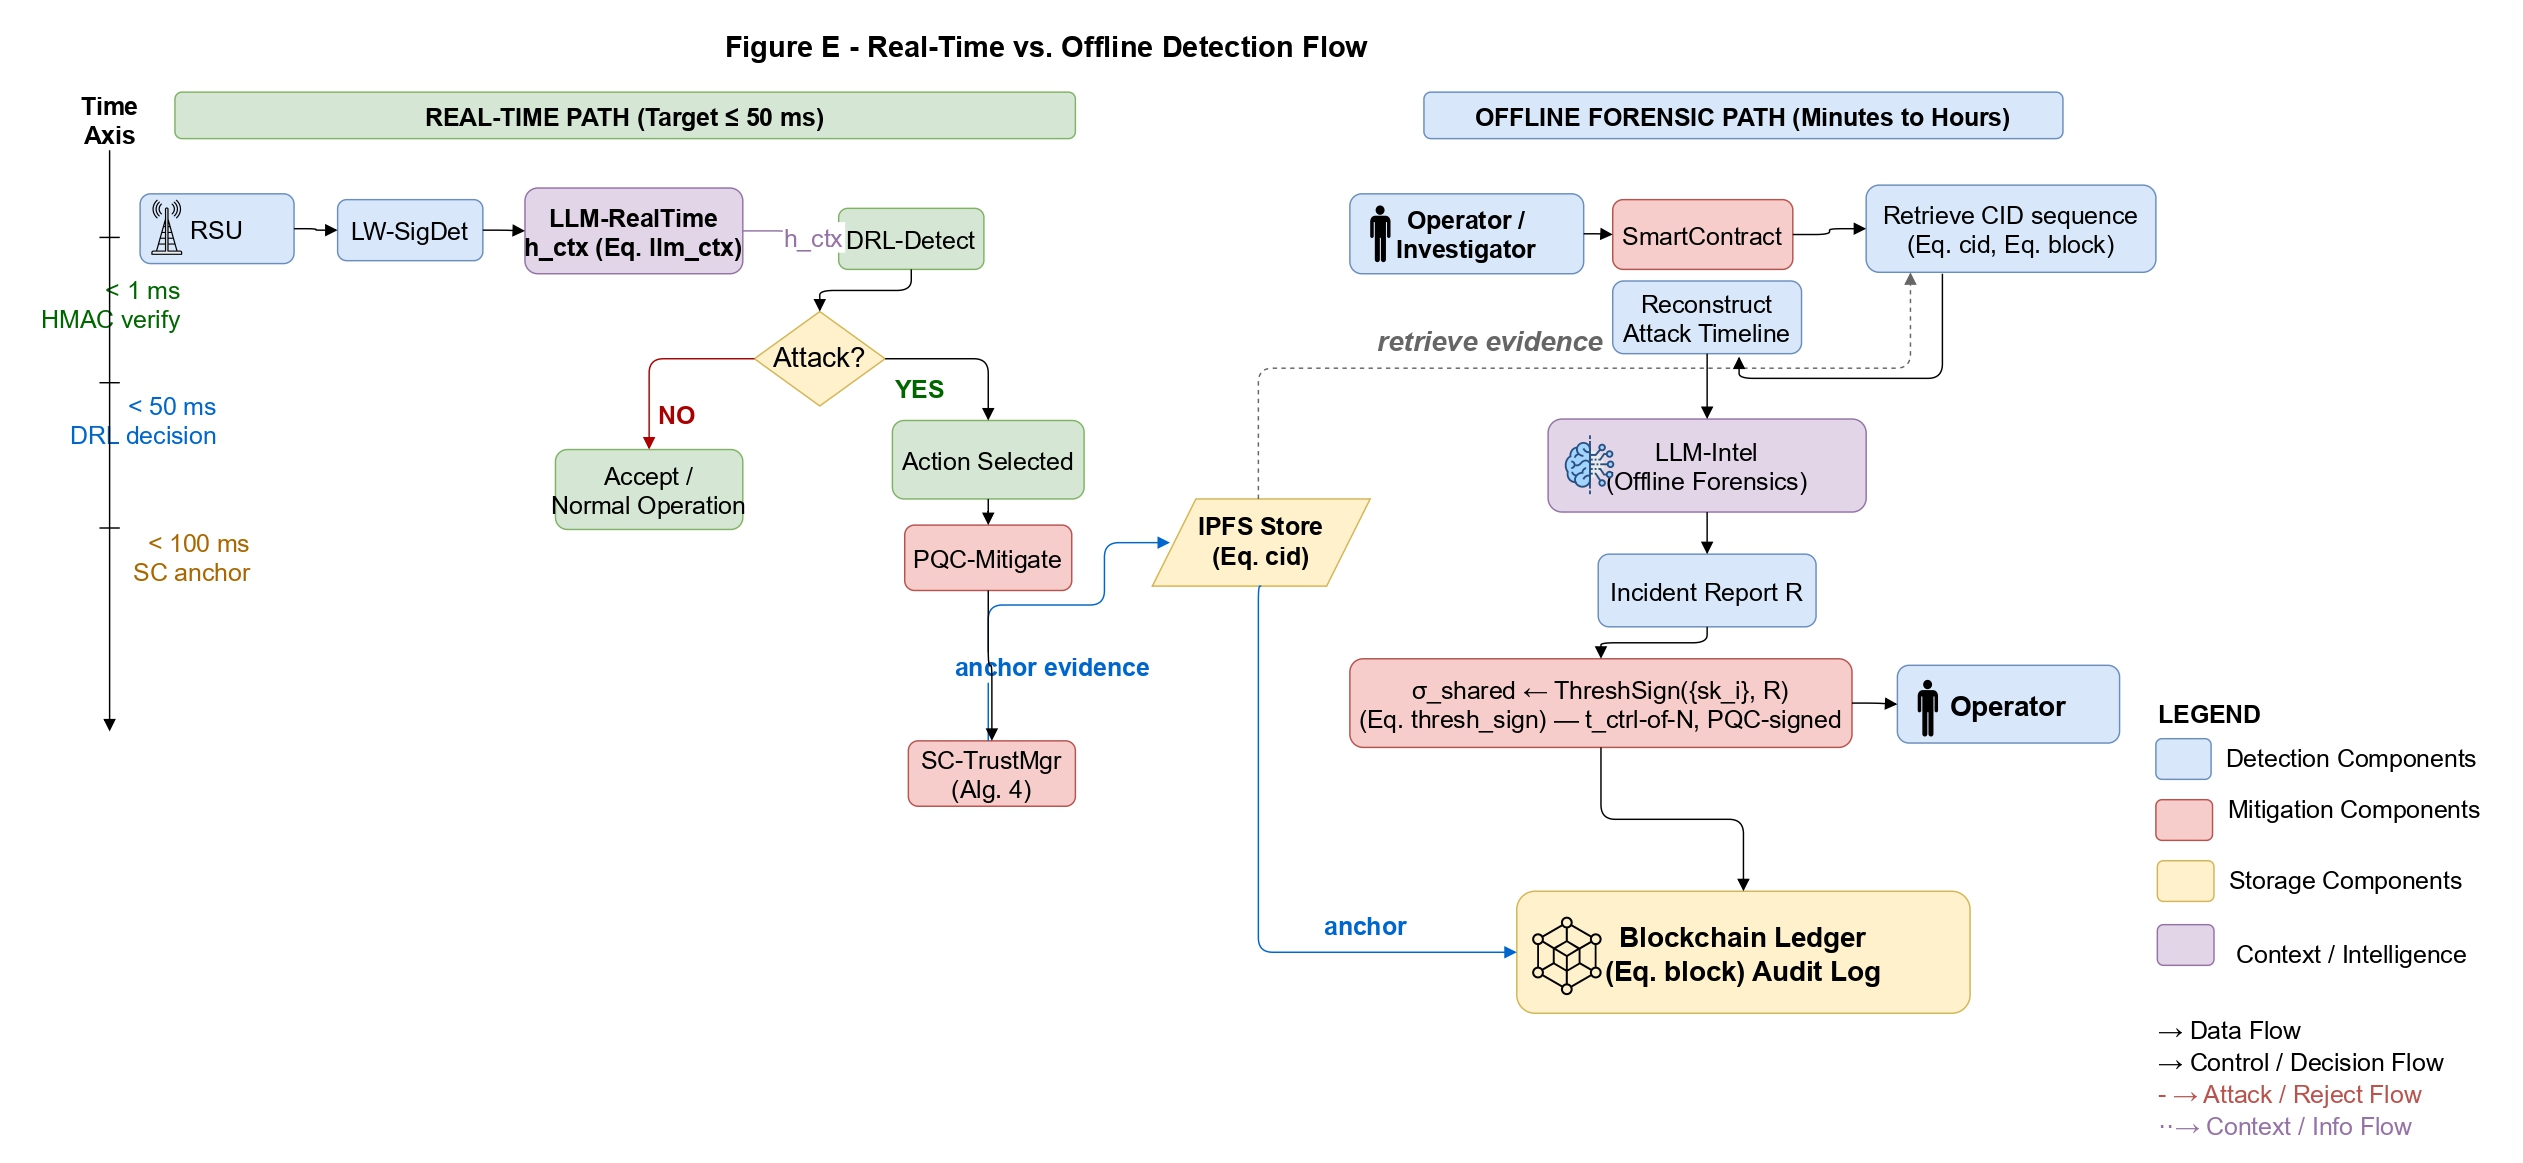
\includegraphics[width=\linewidth]{Progress_Works/DMAP_SDVN/Figure_E_Correct_2.jpg}
\caption{Real-time detection and mitigation path versus offline forensic analysis.}
\label{fig:rt_offline}
\end{figure}
\FloatBarrier
% ====== END FIGURE E ======


As shown in Figure~\ref{fig:rt_offline}, the Real-Time Path
completes HMAC verification in under 1\,ms and DRL-based
detection within 50\,ms, anchoring evidence immediately to
the shared IPFS Store without waiting for blockchain peer
synchronisation. The Offline Forensic Path then reconstructs
the full attack timeline from IPFS-anchored CID sequences and
generates a PQC-signed incident report via LLM-Intel,
ensuring forensic non-repudiation.


\begin{comment}
...
\end{comment}

\subsection{Baseline Selection and Performance Metrics}
\label{sec:baselines}

\subsubsection{External Baselines}

Three external baselines are selected, each addressing the same
general attack class (control-plane or network-layer attacks in
SDN or vehicular networks) and published after 2020.

\begin{enumerate}

\item \textbf{BSD-Guard~\cite{jiang2022bsdguard} (2022).}
A collaborative blockchain-based framework for cooperative
detection and smart-contract-enforced mitigation of SDN control-plane
attacks. Selected because it directly shares the blockchain-SDN
architectural paradigm and control-plane attack class, enabling
direct comparison of both detection performance and mitigation
enforcement latency.

\item \textbf{BCS / Alkhamisi et al.~\cite{alkhamisi2024bcs}
(2024).} A multi-controller SDN blockchain framework with rPBFT
consensus and digit-coin reputation-based attack detection.
Selected as the most recent blockchain-based SDN control-plane
attack detection baseline with a formally defined trust mechanism,
directly comparable to our smart-contract trust-score design.

\item \textbf{DRL-IDS / Satpathy et al.~\cite{satpathy2025cloud}
(2025).} A DRL actor-critic (TD3/DDPG/A2C) intrusion detection
framework with hybrid feature selection and cross-dataset
generalisation evaluation. Selected as the state-of-the-art
DRL detection baseline, enabling direct comparison of DRL
detection performance and inference latency under the same
actor-critic training paradigm.

\end{enumerate}

\subsubsection{Internal Ablation Baselines}

Five ablated variants isolate the contribution of each major
component: \\\textbf{(i)~No-PQC} — ECDSA replaces ML-DSA;
\\\textbf{(ii)~No-DRL} — static adaptive threshold replaces the DRL
agent; \\\textbf{(iii)~No-Blockchain} — timing proofs stored locally
only, no smart-contract enforcement; \\\textbf{(iv)~LW-Only} —
lightweight mode permanently active regardless of threat level;
\\\textbf{(v)~No-LLM} — LLM interpreter removed, alerts generated
by rule-based templates only.

\subsubsection{Performance Metrics}

Six primary metrics evaluate both detection and mitigation impact:

\begin{enumerate}

\item \textbf{Matthews Correlation Coefficient (MCC):} the primary
balanced detection quality metric, robust to class imbalance between
attack and benign timing events across all four attack variants.

\item \textbf{Attack Detection Rate (ADR):} true positive rate
reported per attack variant (DI, RC, SC, SE) and aggregated,
measuring the framework's coverage of the full timing attack surface.

\item \textbf{False Positive Rate (FPR):} false alarm rate measuring
disruption to legitimate control-plane operations — critical for
safety-critical vehicular applications where unnecessary RSU
quarantine directly degrades vehicle coordination.

\item \textbf{Control-Plane Latency Overhead (ms):} additional
end-to-end delay imposed by the defence framework during benign
operation, measured separately for LW and Full modes against a
no-defence baseline.

\item \textbf{Time-to-Mitigate (TTM, ms):} elapsed time from
confirmed attack detection to enforcement of RSU isolation or
path rerouting via smart contract, measuring the speed of the
mitigation role of the blockchain layer.

\item \textbf{Trust Score Accuracy (TSA):} precision and recall
in assigning low trust scores to confirmed compromised RSUs
and maintaining high trust scores for verified benign RSUs
across the simulation duration.

\end{enumerate}

\begin{comment}
\paragraph{Implementation Considerations}
The proposed mitigation strategy is implemented through:
\begin{itemize}
    \item \textbf{PyTorch-based DRL Implementation}: The DRL agent is trained using actor-critic methods on simulated race-condition attack scenarios in NS3.
    
    \item \textbf{Hyperledger Fabric Integration}: Blockchain smart contracts manage RSU trust scores and provide verifiable timing records for event sequence validation.
    
    \item \textbf{Hugging Face Transformers}: LLM modules are fine-tuned on SDVN control-plane event logs to recognize race-condition patterns and generate contextual alerts.
    
    \item \textbf{NS3 Simulation Environment}: Comprehensive testing under various network conditions, mobility patterns, and attack intensities validates the effectiveness of the proposed approach.
\end{itemize}

This integrated defense mechanism provides robust protection against race-condition exploitation attacks by combining adaptive learning with immutable verification and intelligent analysis, ensuring SDVN stability even under sophisticated timing-based attacks.
\end{comment}

\newpage




%%%%%%%%%%%%%%%%%%%%%%%%%%%%%%%%%%%%%%%%%%%%%%%%%%%%%%%%%%%
% \subsection{DRL and LLM Integration}
% \subsubsection{Deep Reinforcement Learning Framework}

% The DRL agent will be implemented in PyTorch and will receive network state observations from NS3 via a socket interface, enabling real-time adaptation to network conditions. The agent will be trained using the SA-GRPO (Security-Aware Group Relative Policy Optimization) algorithm to refine its defense policies through interaction with the simulated SDVN environment.

% The DRL framework architecture includes:
% \begin{itemize}
%     \item \textbf{State Space:} Network topology, flow table status, timing measurements, vehicle mobility patterns, and detected anomalies
%     \item \textbf{Action Space:} Flow rule modifications, path selection decisions, rate limiting adjustments, and alert generation
%     \item \textbf{Reward Function:} Designed to maximize timing accuracy while minimizing false positives and resource consumption
%     \item \textbf{Training Process:} Iterative learning through simulated attack scenarios with progressive difficulty increase
% \end{itemize}

% \subsubsection{Large Language Model Integration}

% A fine-tuned version of a model such as Qwen2.5-7B or Llama-3 will be deployed for intelligent log analysis and threat interpretation. The implementation will utilize Hugging Face's Transformers library and incorporate a Retrieval-Augmented Generation (RAG) system to allow the model to reference the MITRE ATT\&CK framework and previous incident logs.

% Key capabilities include:
% \begin{itemize}
%     \item \textbf{Log Analysis:} Automated parsing and interpretation of timing logs from blockchain, DRL, and network components
%     \item \textbf{Threat Intelligence:} Contextual understanding of attack patterns based on historical data and security frameworks
%     \item \textbf{Alert Generation:} Human-readable security alerts with actionable recommendations
%     \item \textbf{Decision Support:} Intelligent suggestions for defense strategy adjustments based on observed attack patterns
% \end{itemize}

% \subsection{Mathematical Formulation of Timing Integrity}

% To quantify timing anomalies and guide the defense framework, we define rigorous mathematical models for timing deviation detection and defense optimization.

% \subsubsection{Temporal Deviation Metric}

% The "Temporal Deviation" ($\Delta T$) for a control message $m$ is defined as the absolute difference between the actual arrival time at the switch ($T_{obs}$) and the expected time based on the blockchain-validated network state ($T_{exp}$):

% \begin{equation}
% \Delta T_m = |T_{obs} - T_{exp}|
% \end{equation}

% This metric provides a quantitative measure of timing integrity violations. Messages with $\Delta T_m$ exceeding a predetermined threshold are flagged for further analysis by the DRL agent and LLM components.

% \subsubsection{DRL Reward Function}

% The DRL reward function $R_t$ is designed to minimize temporal deviation while penalizing high resource usage ($C$). The function is formulated as:

% \begin{equation}
% R_t = \sum_{m \in M} w_m \cdot e^{-\Delta T_m} - \lambda \cdot C(t)
% \end{equation}

% where:
% \begin{itemize}
%     \item $w_m$ represents the priority weight of message $m$, with safety-critical messages (e.g., collision warnings, emergency vehicle notifications) assigned higher weights
%     \item $\lambda$ is a scaling factor that balances timing accuracy against computational overhead
%     \item $M$ denotes the set of control messages processed in time period $t$
%     \item $C(t)$ represents the cumulative computational cost of defense operations at time $t$
% \end{itemize}

% The exponential term $e^{-\Delta T_m}$ ensures that the reward decreases rapidly as timing deviation increases, encouraging the DRL agent to prioritize timing accuracy. The resource penalty term prevents the agent from deploying computationally expensive defense mechanisms unnecessarily.

% \subsection{Implementation Workflow}

% The complete implementation will follow a systematic workflow:

% \begin{enumerate}
%     \item \textbf{Environment Setup:} Configure NS3 simulation environment with SDVN topology and SUMO mobility traces
%     \item \textbf{Baseline Characterization:} Establish baseline performance metrics under normal operating conditions
%     \item \textbf{Attack Implementation:} Develop and deploy timing attack scenarios including delay injection, race conditions, side-channel attacks, and synchronization exploits
%     \item \textbf{Blockchain Deployment:} Initialize consortium blockchain network and deploy timing consensus smart contracts
%     \item \textbf{DRL Training:} Train the reinforcement learning agent through iterative exposure to attack scenarios
%     \item \textbf{LLM Fine-tuning:} Adapt the large language model using domain-specific security logs and threat intelligence
%     \item \textbf{Integration Testing:} Validate seamless operation of all components in the integrated defense framework
%     \item \textbf{Performance Evaluation:} Conduct comprehensive experiments measuring detection rate, false positive rate, latency impact, and resource overhead
% \end{enumerate}

% \subsection{Expected Research Outputs and Significance}

% This project aims to produce high-impact research outputs, including journal publications and conference presentations in the domains of vehicular networking and cybersecurity. The significance of this work extends beyond academic novelty:

% \subsubsection{Safety Enhancement}

% By mitigating timing attacks, we directly prevent real-world traffic accidents and improve the reliability of autonomous coordination. The framework ensures that safety-critical messages such as collision warnings and emergency alerts maintain their timing integrity, protecting both passengers and pedestrians.

% \subsubsection{Architectural Robustness}

% The "trustless" control plane provides a blueprint for securing other critical infrastructure that utilizes SDN, such as smart grids or industrial IoT systems. The principles developed in this research can be adapted to any time-sensitive networked system where control plane security is paramount.

% \subsubsection{Intelligent Automation}

% This work demonstrates the first fully automated "SecLoop" in vehicular networks, reducing the burden on human security analysts in the upcoming 6G and zero-touch network era. The combination of blockchain verification, DRL adaptation, and LLM intelligence creates a self-healing security system capable of responding to emerging threats without manual intervention.